% Template KLTN cho SV trường ĐHKHTN
% Liên hệ: nqminh@fit.hcmus.edu.vn
% Last update: 08/06/2016

% Chú ý: đọc các phần chú ý đóng khung của file này và chỉnh lại cho phù hợp.
% Trước khi build, xóa hết các file được tạo ra trong quá trình build trước đó, và build theo thứ tự: BIB > PDF > PDF.
% Nếu cập nhật tài liệu tham khảo, cũng cần build lại theo cách trên.

\documentclass[oneside,a4paper,14pt]{extreport}

% Utilities
\usepackage{systeme}
\usepackage{hhline}
\usepackage{nicematrix}
\usepackage[export]{adjustbox}
\usepackage{subcaption}
\usepackage{enumerate}
\usepackage{enumitem}
\usepackage{tikz}
\usepackage{sepfootnotes}
\usepackage{tablefootnote}
\usepackage{svg}
\usetikzlibrary{calc, graphs, fit, arrows.meta}
\definecolor{airforceblue}{HTML}{4677B8}
\definecolor{fireenginered}{HTML}{CE4949}
\definecolor{asparagus}{HTML}{8DCE49}
\definecolor{cadmiumorange}{rgb}{0.93, 0.53, 0.18}
\definecolor{goldenyellow}{HTML}{f7f379}
\definecolor{darklavender}{HTML}{8D49D1}
\definecolor{electriccyan}{HTML}{6FE8E8}

% Font
\usepackage{bm}
\usepackage{amsfonts}

% Font tiếng Việt
\usepackage[T5]{fontenc}
\usepackage[utf8]{inputenc}
\DeclareTextSymbolDefault{\DH}{T1}

% Tài liệu tham khảo
\usepackage[
        sortcites,
	sorting=nty,
	backend=biber,
	defernumbers=true,
        maxbibnames=99,
        giveninits=true
 ]{biblatex}
\usepackage[unicode]{hyperref} % Bookmark tiếng Việt
\addbibresource{References/references.bib}

\makeatletter
\def\blx@maxline{77}
\makeatother

% Chèn hình, các hình trong luận văn được để trong thư mục Images/
\usepackage{graphicx,float}
\graphicspath{ {Images/} }

% Chèn và định dạng mã nguồn
\usepackage{listings}
\usepackage{color}
\definecolor{codegreen}{rgb}{0,0.6,0}
\definecolor{codegray}{rgb}{0.5,0.5,0.5}
\definecolor{codepurple}{rgb}{0.58,0,0.82}
\definecolor{backcolour}{rgb}{0.95,0.95,0.92}
\lstdefinestyle{mystyle}{
    backgroundcolor=\color{backcolour},   
    commentstyle=\color{codegreen},
    keywordstyle=\color{magenta},
    numberstyle=\tiny\color{codegray},
    stringstyle=\color{codepurple},
    basicstyle=\footnotesize,
    breakatwhitespace=false,         
    breaklines=true,                 
    captionpos=b,                    
    keepspaces=true,                 
    numbers=left,                    
    numbersep=5pt,                  
    showspaces=false,                
    showstringspaces=false,
    showtabs=false,                  
    tabsize=2
}
\lstset{style=mystyle}

% Chèn và định dạng mã giả
\usepackage{amsmath}
\usepackage{yhmath}
\usepackage{amssymb}
\usepackage{algorithm}
\usepackage[noend]{algpseudocode}
\makeatletter
\def\BState{\State\hskip-\ALG@thistlm}
\makeatother

% Bảng biểu
\usepackage{multirow}
\usepackage{array}
\usepackage{booktabs}
\newcolumntype{L}[1]{>{\raggedright\let\newline\\\arraybackslash\hspace{0pt}}m{#1}}
\newcolumntype{C}[1]{>{\centering\let\newline\\\arraybackslash\hspace{0pt}}m{#1}}
\newcolumntype{R}[1]{>{\raggedleft\let\newline\\\arraybackslash\hspace{0pt}}m{#1}}
\newcolumntype{P}[1]{>{\centering\arraybackslash}p{#1}}
\newcolumntype{M}[1]{>{\centering\arraybackslash}m{#1}}

% Đổi tên mặc định
\renewcommand{\chaptername}{Chương}
\renewcommand{\figurename}{Hình}
\renewcommand{\tablename}{Bảng}
\renewcommand{\contentsname}{Mục lục}
\renewcommand{\listfigurename}{Danh sách hình}
\renewcommand{\listtablename}{Danh sách bảng}
\renewcommand{\appendixname}{Phụ lục}

% Dãn dòng 1.5
\usepackage{setspace}
\onehalfspacing

% Thụt vào đầu dòng
\usepackage{indentfirst}

% Canh lề
\usepackage[
  top=30mm,
  bottom=25mm,
  left=30mm,
  right=20mm,
  includefoot]{geometry}
  
% Trang bìa
\newcommand\HRule{\rule{\textwidth}{1pt}}

% ========================================================================================= %
% CHÚ Ý: Thông tin chung về KLTN - sinh viên điền vào đây để tự động update các trang khác  %
% ========================================================================================= %
\newcommand{\tenSV}{Hồ~Trần~Việt~Cường~-~Nguyễn~Trung~Dũng} % Dấu ~ là khoảng trắng không được tách (các chữ nối với nhau bằng dấu ~ sẽ nằm cùng 1 dòng
\newcommand{\mssv}{19120056-19120486}
\newcommand{\tenKL}{Sử~dụng~LaTeX trong Khoá~luận~tốt~nghiệp} % Chú ý dấu ~ trong tên khóa luận
\newcommand{\tenGVHD}{GS.TS~Lê~Hoài~Bắc}
\newcommand{\tenBM}{Khoa học máy tính}

\begin{document}

\begin{titlepage}

\begin{center}
%ĐẠI HỌC QUỐC GIA THÀNH PHỐ HỒ CHÍ MINH\\
TRƯỜNG ĐẠI HỌC KHOA HỌC TỰ NHIÊN\\
\textbf{KHOA CÔNG NGHỆ THÔNG TIN}\\[2cm]


{ \Large \bfseries Hồ Trần Việt Cường -- Nguyễn Trung Dũng\\[2cm] } 

%Tên đề tài Khóa luận tốt nghiệp/Đồ án tốt nghiệp

{ \Large \bfseries HỌC TỰ GIÁM SÁT\\TRÊN MẠNG HỌC SÂU ĐỒ THỊ\\CHO HỆ THỐNG GỢI Ý\\[3cm]} 


%Chọn trong các dòng sau
\large KHÓA LUẬN TỐT NGHIỆP\\
%\large ĐỒ ÁN TỐT NGHIỆP CỬ NHÂN\\
%\large THỰC TẬP TỐT NGHIỆP CỬ NHÂN\\
%Đưa vào dòng này nếu thuộc chương trình Chất lượng cao, hoặc lớp Cử nhân tài năng
\large CHƯƠNG TRÌNH CHÍNH QUY\\
%\large CHƯƠNG TRÌNH CHẤT LƯỢNG CAO\\
%\large CHƯƠNG TRÌNH CỬ NHÂN TÀI NĂNG\\[2cm]


\begin{tikzpicture}[remember picture, overlay]
  \draw[line width = 2pt] ($(current page.north west) + (2cm,-2cm)$) rectangle ($(current page.south east) + (-1.5cm,2cm)$);
\end{tikzpicture}

\vfill
Tp. Hồ Chí Minh, tháng 6/2023

\end{center}

\pagebreak



\begin{center}

TRƯỜNG ĐẠI HỌC KHOA HỌC TỰ NHIÊN\\
\textbf{KHOA CÔNG NGHỆ THÔNG TIN}\\[2cm]


{\large \bfseries Hồ Trần Việt Cường -- 19120056\\} 
{\large \bfseries Nguyễn Trung Dũng -- 19120486\\[2cm]}

%Tên đề tài Khóa luận tốt nghiệp/Đồ án tốt nghiệp


{ \Large \bfseries HỌC TỰ GIÁM SÁT\\TRÊN MẠNG HỌC SÂU ĐỒ THỊ\\CHO HỆ THỐNG GỢI Ý \\[2cm]}  


%Chọn trong các dòng sau
\large KHÓA LUẬN TỐT NGHIỆP\\
%\large ĐỒ ÁN TỐT NGHIỆP CỬ NHÂN\\
%Đưa vào dòng này nếu thuộc chương trình Chất lượng cao, hoặc lớp Cử nhân tài năng
\large CHƯƠNG TRÌNH CHÍNH QUY\\[2cm]
%\large CHƯƠNG TRÌNH CHẤT LƯỢNG CAO\\[2cm]
%\large CHƯƠNG TRÌNH CỬ NHÂN TÀI NĂNG\\[2cm]

\textbf{GIẢNG VIÊN HƯỚNG DẪN}\\
GS.TS. Lê Hoài Bắc\\


\begin{tikzpicture}[remember picture, overlay]
  \draw[line width = 2pt] ($(current page.north west) + (2cm,-2cm)$) rectangle ($(current page.south east) + (-1.5cm,2cm)$);
\end{tikzpicture}

\vfill
Tp. Hồ Chí Minh, tháng 06/2023

\end{center}
\thispagestyle{empty}
\end{titlepage}
% Sasu trang Title, các bạn chèn nhận xét gủa GVHD và GVPB. Nhận xét sẽ được giáo vụ phát sau buổi bảo vệ để các bạn đóng quyển.

\pagenumbering{roman} % Đánh số i, ii, iii, ...

%\addcontentsline{toc}{chapter}{Lời cam đoan}
%\chapter*{Lời cam đoan}
\label{reassurances}

Tôi xin cam đoan đây là công trình nghiên cứu của riêng tôi. Các số liệu và kết quả nghiên cứu trong luận văn này là trung thực và không trùng lặp với các đề tài khác.

\addcontentsline{toc}{chapter}{Lời cảm ơn}
\chapter*{Lời cảm ơn}
\label{thanks}

\noindent Lời đầu tiên, chúng em xin phép gửi lời cám ơn chân thành, sâu sắc đến thầy Lê Hoài Bắc vì đã tận tâm hỗ trợ, gửi những lời khuyên, lời động viên trong suốt quãng thời gian nhóm thực hiện khóa luận. Cảm ơn thầy đã luôn theo dõi quá trình hoạt động của nhóm, kịp thời đưa ra những lời khuyên để nhóm có thể hoàn thành khóa luận đến ngày hôm nay.

Chúng em xin phép gửi lời cám ơn đến quý thầy cô trường Đại học Khoa học Tự nhiên nói chung và khoa Công nghệ Thông tin nói riêng vì đã luôn nhiệt tình chỉ dạy những bài học, những kinh nghiệm quý giá, là hành trang vững chắc cho chúng em trong suốt quãng thời gian được học tập ở trường vừa qua.

Chúng em xin phép gửi lời cám ơn đến gia đình, bạn bè những người đã luôn đồng hành, luôn túc trực động viên trong suốt quãng thời gian vừa gian để chúng em có thể đạt được kết quả tốt nhất.

Lời cuối cùng, chúng em xin phép kính chúc quý thầy cô, gia đình, bạn bè -- những người đã đóng góp một phần công lao không hề nhỏ cho thành quả của chúng em ngày hôm nay một lời chúc sức khỏe, bình an, hạnh phúc trong cuộc sống.

\addcontentsline{toc}{chapter}{Đề cương chi tiết}
\include{Appendix/decuong}

% Mục lục, danh sách hình, danh sách bảng
\addcontentsline{toc}{chapter}{Mục lục}
\tableofcontents
\listoffigures
\listoftables

\addcontentsline{toc}{chapter}{Tóm tắt}
\chapter*{Tóm tắt}
\label{summary}
% Trình bày tóm tắt vấn đề nghiên cứu, các hướng tiếp cận, cách giải quyết vấn đề và một số kết quả đạt được.

\noindent Con người luôn mong muốn giảm bớt gánh nặng trong việc suy nghĩ và lựa chọn, doanh nghiệp thì luôn muốn bán được nhiều sản phẩm hơn. Xây dựng hệ thống gợi ý là bài toán không mới, tuy nhiên việc xây dựng sao cho hiệu quả thực sự vẫn đang là một bài toán tồn tại rất nhiều vấn đề vẫn chưa thể giải quyết triệt để. Rất nhiều các phương pháp được đề xuất, nhìn chung ta vẫn đang phải đối mặt với các vấn đề như dữ liệu thưa hay việc học biểu diễn từ đồ thị tương tác người dùng -- sản phẩm đang chịu ảnh hưởng nhiều bởi nhiễu. Điều này thúc đẩy động lực cho các phương pháp học mới ra đời với mục tiêu là hạn chế tác động của dữ liệu thưa và tăng độ chịu nhiễu của mô hình.

Mạng học sâu đồ thị đã chứng minh được tính hiệu quả khi áp dụng lên hệ thống gợi ý dựa trên việc khai thác cấu trúc đồ thị tương tác của người dùng. Hầu hết các bộ dữ liệu được sử dụng để huấn luyện các mô hình học gợi ý đều rất thưa, điều này dẫn tới việc huấn luyện và đánh giá các mô hình này đều cho kết quả không tốt. Mô hình Học tự giám sát ra đời và được áp dụng rất thành công trong lĩnh vực thị giác máy tính và xử lý ngôn ngữ tự nhiên và có tiềm năng rất lớn trong cả lĩnh vực học đồ thị.

Khóa luận này nhằm mục đích nghiên cứu các vấn đề xoay quanh việc áp dụng \textbf{Học tự giám sát lên mạng học sâu đồ thị cho hệ thống gợi ý}. Bằng cách sử dụng Học tương phản -- một hướng tiếp cận của Học tự giám sát bổ trợ cho tác vụ gợi ý, thuật toán đề xuất của khóa luận đã đạt hiệu quả cao trên những tập dữ liệu rất thưa khi so sánh với các mô hình sử dụng mạng học sâu đồ thị cho hệ thống gợi ý khác.


\clearpage

\pagenumbering{arabic} % Đánh số 1, 2, 3, ...

% Các chương nội dung
\chapter{Giới thiệu}
\label{Chapter1}

%Tóm tắt luận văn được trình bày nhiều nhất trong 24 trang in trên hai mặt giấy, cỡ chữ Times New Roman 11 của hệ soạn thảo Winword hoặc phần mềm soạn thảo Latex đối với các chuyên ngành thuộc ngành Toán.

%Mật độ chữ bình thường, không được nén hoặc kéo dãn khoảng cách giữa các chữ.
%Chế độ dãn dòng là Exactly 17pt.
%Lề trên, lề dưới, lề trái, lề phải đều là 1.5 cm.
%Các bảng biểu trình bày theo chiều ngang khổ giấy thì đầu bảng là lề trái của trang.
%Tóm tắt luận án phải phản ảnh trung thực kết cấu, bố cục và nội dung của luận án, phải ghi đầy đủ toàn văn kết luận của luận án.
%Mẫu trình bày trang bìa của tóm tắt luận văn (phụ lục 1).

\noindent Trong chương này, nhóm nghiên cứu sẽ phát biểu về bài toán xây dựng hệ thống gợi ý, cũng như đóng góp của nó cho cuộc sống của con người đến nay. Tiếp theo, ta sẽ trình bày về vấn đề dữ liệu thưa, một trong những vấn đề nhức nhối, bắt gặp nhiều nhất khi xây dựng một hệ thống gợi ý. Để giải quyết vấn đề này, phương pháp ``Học tự giám sát'' được sử dụng nhằm hạn chế tác động do dữ liệu thưa mang lại cho hệ thống. Phạm vi và phương pháp nghiên cứu sẽ được mô tả một cách tổng quát. Bố cục cũng sẽ được đề cập tới nhằm cho người đọc có thể nắm được toàn cảnh hoạt động nghiên cứu.

\section{Đặt vấn đề và Động lực}

\noindent Việc con người nhận được ngay những gợi ý, những quảng cáo từ các nền tảng ví dụ như mảng xã hội, sàn thương mại điện tử,... sau khi phát sinh lịch sử tương tác đã không còn quá xa lạ. Con người tương tác với sản phẩm dưới bất kỳ hình thức nào như xem sản phẩm, đặt mua sản phẩm, đánh giá sản phẩm,... đều rất đáng giá và được một số loại hệ thống ghi lại. Hệ thống gợi ý dựa trên lịch sử tương tác của người dùng hỗ trợ ra quyết định, cung cấp các gợi ý cho người dùng về những ``sản phẩm'' mà họ có thể cần. Ví dụ, sau khi xem một bộ phim trên Netflix, ta được gợi ý những bộ phim có thể loại tương tự, hay khi ta mua điện thoại, hệ thống sẽ gợi ý cho ta những phụ kiện điện thoại thường được mua kèm. Với những ``sản phẩm'' đúng, ta có thể mang lại trải nghiệm tốt cho người dùng, xa hơn là có thể thúc đẩy phát triển kinh doanh. Dưới kỷ nguyên 4.0, không gian tương tác ngày một lớn, trong khí đó người dùng có khuynh hướng chỉ tương tác với một phần rất nhỏ trong cơ sở dữ liệu. Điều này đã trở thành một động lực to lớn, thúc đẩy việc tìm ra một phương pháp hạn chế tác động tiêu cực đến từ chính bản thân dữ liệu này.

Bất kỳ dạng bài nào, ta cũng phải xác định rõ đầu vào, đầu ra (mục tiêu) của bài toán đó, mục tiêu của bài toán là gì. Vậy đầu vào, đầu ra của bài toán này là gì? Ở đầu vào, ta cần đưa cho hệ thống gợi ý lịch sử tương tác với ``sản phẩm'' của một hoặc nhiều người dùng. Đầu ra của hệ thống sẽ dự đoán về hành vi, ``sản phẩm'' của người dùng có thể thích hay cần ở hiện tại hoặc tương lai.

Bất kỳ bài toán nào, cũng tồn tại những vấn đề của riêng nó. Bài toán hệ thống gợi ý đang phải giải quyết một số vấn đề  như dữ liệu thưa. Trong ngữ cảnh của hệ thống gợi ý, đa phần người dùng sẽ chỉ tương tác với một phần rất nhỏ trong một lượng lớn các ``sản phẩm'' tồn tại trong cơ sở dữ liệu. Điều này sẽ gây khó khăn cho việc tìm ra những người dùng ``giống nhau''. Bên cạnh đó, hành vi của người dùng chịu ảnh hưởng bởi tác động của rất nhiều yếu tố. Tập hợp những điều đó lại, có thể dẫn đến việc sai lệch trong quá trình đưa ra gợi ý.

Bài toán xây dựng hệ thống gợi ý là bài toán không mới, tuy nhiên nó cũng chỉ mới nở rộ cách đây không lâu \cite{survey:sota-rec-system}, và cũng còn rất nhiều tiềm năng để phát triển. Học sâu đã mở ra một chương mới cho bài toán xây dựng hệ thống gợi ý, điều này minh chứng bằng việc sự phát triển nhanh chóng mà các mô hình học sâu mang lại dạo thời gian gần đây. Mạng học sâu đồ thị, học tăng cường, học tự giám sát là một vài chủ đề trong những chủ đề đang nhận được khá nhiều quan tâm hiện tại. Học tự giám sát chủ đề nghiên cứu chính được trình bày trong khóa luận này.

Học giám sát (Supervised Learning) cần một lượng lớn dữ liệu được gán nhãn cẩn thận để đem lại hiệu quả tốt. Việc này đòi hỏi một lượng lớn thời gian, tiền bạc để gán nhãn và điều này quả thực là rất tốn kém. Trong khi đó, lượng dữ liệu chưa được gán nhãn thì lại rất nhiều và liên tục được sinh ra, nếu ta chăm chăm vào việc làm sao để gán nhãn thì sẽ không kịp các tiến trình học. Gần đây, Học tự giám sát (Self-supervised Learning) là một hướng nghiên cứu mới được đưa ra và nhận được khá nhiều sự quan tâm, có tiềm năng giải quyết/hạn chế một phần các vấn đề của hệ thống gợi ý (ví dụ điển hình như dữ liệu thưa).

Bằng cách sử dụng học tự giám sát, ta có thể tận dụng lượng dữ liệu không gán nhãn, học từ chính những đặc trưng bên trong của dữ liệu, cải tiến hiệu quả của toàn bộ hệ thống. Học tự giám sát được áp dụng trong rất nhiều lĩnh vực nghiên cứu, và là hướng nghiên cứu đang còn rất mới kể cả trong lĩnh vực xử lý ảnh hay ngôn ngữ tự nhiên, việc áp dụng mô hình học này vào bài toán hệ thống gợi ý lại càng mới hơn. Ở phần tiếp theo, mục tiêu nghiên cứu của khóa luận sẽ được trình bày kỹ hơn.

\section{Mục tiêu nghiên cứu}

\noindent Như đã đề cập, học tự giám sát là một trong những phương pháp đáng hứa hẹn với hi vọng giải quyết được các vấn đề còn vướng phải của hệ thống gợi ý ở hiện tại và tương lai. 

Với đề tài này, ta cần biết được tình hình nghiên cứu về mạng học sâu đồ thị cho hệ thống gợi ý cũng như việc áp dụng học tự giám sát vào bài toán này trong thời gian gần đây. Qua đó biết được các hướng nghiên cứu đã và đang được hướng tới, hướng nào tốt hoặc chưa tốt ở điểm nào, các vấn đề đã giải quyết được cũng như các vấn đề vẫn cần phải quyết trong tương lai.

Điều căn bản nhất, ta cần hiểu rõ được lý thuyết xoay quanh bài toán học giám sát trên mạng học sâu đồ thị cho hệ thống gợi ý. Đầu tiên là về hệ thống gợi ý; tiếp theo là về mạng học sâu đồ thị - một loại mạng học sâu đã và đang được nhiều công trình nghiên cứu hướng tới áp dụng, cách áp dụng mạng học sâu này lên hệ thống gợi ý như thế nào; ta cũng biết được có những cách nào để áp dụng mô hình học tự giám sát - một phương pháp được áp dụng trên mạng học sâu không chỉ trên hình ảnh, văn bản mà thậm chí có thể sử dụng với đồ thị một cách hiệu quả. Từ đó có thể nắm vững kiến thức nền tảng một cách có hệ thống.

Không kém phần quan trọng, ta cần nghiên cứu và cài đặt những gì nghiên cứu được. Cụ thể, đề tài này sẽ đi theo ý tưởng chính của Wu \cite{SGL} và tiến hành cài đặt lại học tự giám sát trên mạng học sâu đồ thị, nhằm chứng minh được hiệu quả mang lại của phương pháp này vào bài toán hệ thống gợi ý. Bên cạnh đó, ta cũng sẽ tiến hành tìm hiểu, thử nghiệm một số cải tiến nhằm giải quyết những điểm chưa tốt của mô hình hiện tại. Việc này nhằm nhìn nhận lại vấn đề và giải quyết một phần nào đó những hạn chế mà hướng nghiên cứu hiện tại đang gặp phải. Từ đó mở ra cơ hội khai thác sâu hơn hoặc tìm ra được các hướng nghiên cứu mới hơn, hiệu quả hơn trong bài toán hệ thống gợi ý.

\section{Phạm vi nghiên cứu}

\noindent 3 bộ dữ liệu thường được sử dụng trong các đề tài nghiên cứu về mạng học sâu đồ thị cho hệ thống gợi ý được đề tài chọn để tiến hành thí nghiệm:
\begin{itemize}
    \item[(1)] Yelp 2018: bộ dữ liệu của Yelp, chứa thông tin về doanh nghiệp, người dùng, và đánh giá của người dùng về các doanh nghiệp đó.

    \item[(2)] Amazon Book: thông tin đánh giá của người dùng từ Amazon trong khoảng từ năm 1996 đến 2014.

    \item[(3)] Alibaba iFashion: bộ dữ liệu công khai của Alibaba, gồm các sản phẩm thời trang của trang bán hàng online và các tương tác của người dùng.
\end{itemize}
Chi tiết cụ thể về các bộ dữ liệu sẽ được đề cập ở phần sau.

Đề tài sẽ tập trung về việc giải thích học tự giám sát trên mạng học sâu đồ thị được áp dụng vào hệ thống gợi ý. Bên cạnh đó, một số thí nghiệm sẽ được tiến hành nhằm cải tiến thêm dựa trên những vấn đề đang gặp phải của hệ thống bên trên.

Trong suốt quá trình thực hiện đề tài, những hạn chế của nghiên cứu sẽ được thừa nhận, giải quyết. Những kết quả sẽ được giải thích và thảo luận những yếu tố tác động. Các nghiên cứu trong tương lai có thể  được tiến hành mở rộng dựa trên kết quả của nghiên cứu này và giải quyết những thiếu sót mà hiện tại vẫn chưa giải quyết được. Nhìn chung, nghiên cứu này sẽ cung cấp những kiến thức nền tảng, nâng cao hiểu biết về những tiềm năng còn khai phá được trong lĩnh vực hệ thống gợi ý nhằm nâng cao hiệu quả của mô hình này nói chung và hướng nghiên cứu, áp dụng mô hình học học tự giám sát vào hệ thống này nói riêng.

\section{Phương pháp nghiên cứu}

\noindent Như ta có đề cập rằng việc gán nhãn cho bộ dữ liệu quả thực là một điều cực kỳ tốn kém. Việc gán nhãn cho bài toán sử dụng bộ dữ liệu dạng hình ảnh, văn bản có thể sẽ dễ dàng hơn so với bài toán hệ thống gợi ý. Lúc này, dữ liệu được tạo ra bởi chính bản thân người dùng, người dùng tương tác với sản phẩm và để lại đánh giá của riêng mình. Tuy nhiên, đa số người dùng chỉ tương tác với một phần nhỏ các mục/vật phẩm so với toàn bộ vật phẩm mà họ có thể tương tác tới. Vì vậy, vấn đề về dữ liệu huấn luyện vẫn luôn là một chướng ngại gây cản trở các mô hình gợi ý học sâu có thể đạt được tiềm năng của nó.

Tất nhiên là không phải lúc nào dữ liệu cũng được gán nhãn sẵn. Trong nhiều trường hợp thực tế, ta phải đối mặt với một lượng lớn dữ liệu không nhẵn (có thể là chưa gán nhãn hoặc thậm chí không thể gán nhãn). Với học tự giám sát, mô hình có thể học được từ chính những đặc trưng bên trong của dữ liệu, từ đó cải thiện độ chính xác của mô hình. 

Để cải thiện hệ thống gợi ý, ta có thể áp dụng nó đồng thời với tác vụ học tự giám sát (self-supervised learning). Cụ thể, mô hình sẽ được huấn luyện bằng cách để tác vụ gợi ý đóng vai trò chính; học tự giám sát, cụ thể hơn là học tương phản (contrastive learning) với vai trò bổ trợ nhằm tối ưu cho mô hình gợi ý cổ điển. Để áp dụng được học tương phản, ta sẽ cần rất nhiều dữ liệu và hiển nhiên bộ dữ liệu gốc (bộ dữ liệu hạn chế) mà ta có ban đầu sẽ không đáp ứng được điều này. Tăng cường dữ liệu (data augmentation) -- một kỹ thuật nhằm tăng thêm dữ liệu từ chính dữ liệu mà ta hiện có, được áp dụng rất nhiều trên dữ liệu dạng hình ảnh, văn bản cũng mang lại kết quả khá khả quan trong các công trình nghiên cứu dạo gần đây trên dữ liệu dạng đồ thị. Không khác về mặt ý tưởng, khi áp dụng đồ thị, tăng cường dữ liệu hoạt động bằng cách tạo ra các biến thể (view) khác nhau từ đồ thị gốc ban đầu, các biến thể này vẫn giữ đuợc đặc trưng, cấu trúc từ đồ thị gốc. Với các biến thể mới được tạo ra này, ta có thể học được cách biểu diễn một cách tốt hơn từ việc khiến các biến thể khác nhau của cùng một node tiến lại gần nhau, khác node đẩy ra xa nhau. Từ đó, cải thiện hiệu suất chung cho toàn bộ hệ thống.

\begin{figure}[H]
    \centering
    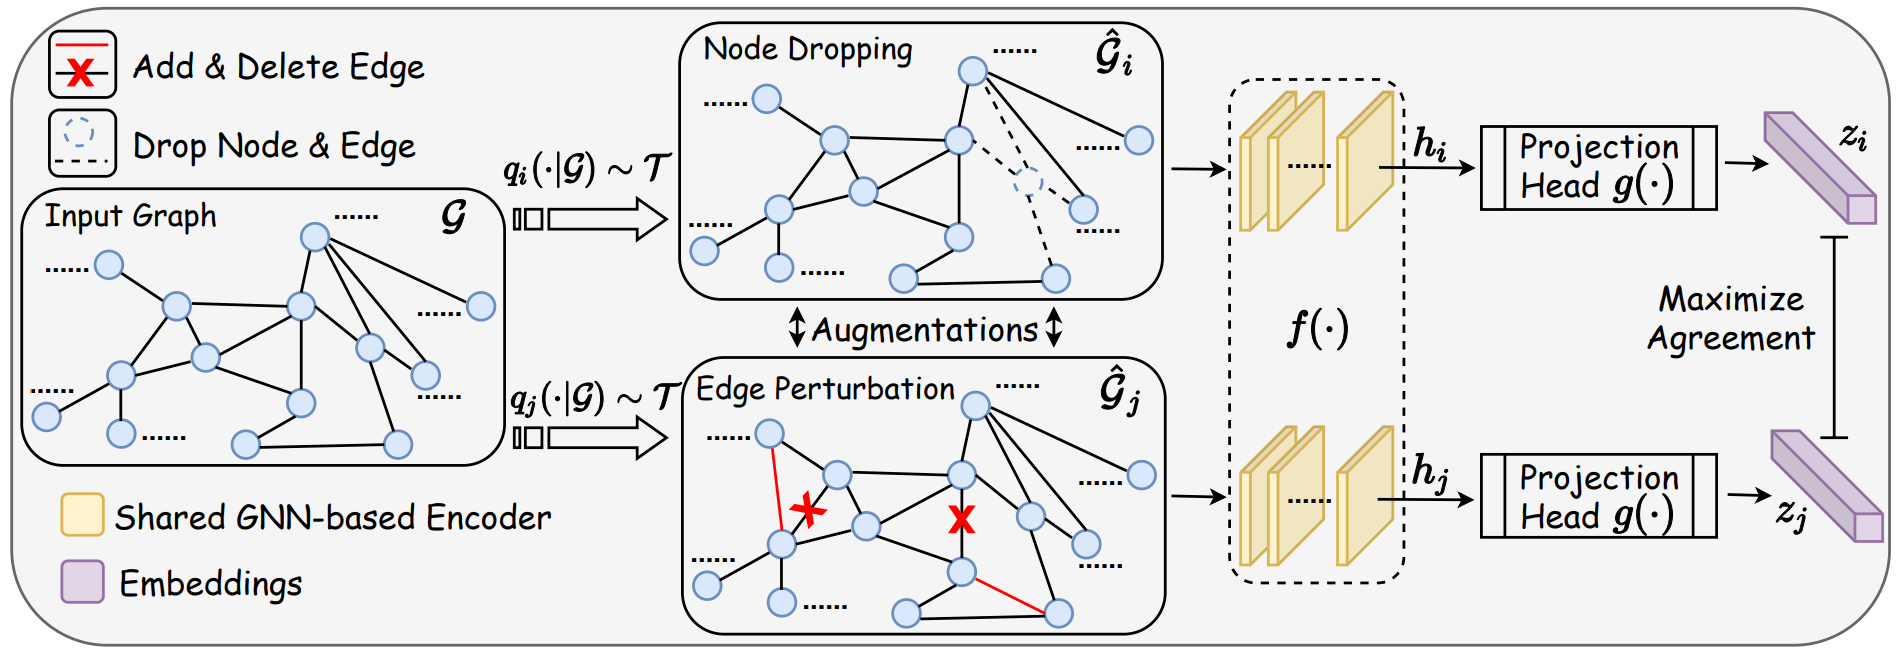
\includegraphics[scale=0.31]{images/Chapter1/graph-contrastive-learning.png}
    \caption{Ví dụ về việc tạo ra các view dẫn tới việc tác dộng đến học biểu diễn.}
\end{figure}

\section{Bố cục}

\noindent Ở chương này, ta cũng đã trình bày về vai trò của hệ thống gợi ý trong cuộc sống, cũng như cho thấy được rằng, hệ thống gợi ý nói chung và học tự giám sát trên hệ thống gợi ý nói riêng vẫn còn rất mới và thực sự có rất nhiều tiềm năng để đầu tư nghiên cứu. Phần còn lại của khóa luận sẽ trình bày theo thứ tự như sau:
\begin{itemize}
    \item[] \textbf{Chương 2}: Trình bày các kiến thức nền tảng về hệ thống gợi ý, mạng học sâu đồ thị, tăng cường dữ liệu và mô hình Học tự giám sát (Self-supervised Learning).
    
    \item[] \textbf{Chương 3}: Trình bày về việc áp dụng học tự giám sát lên mạng học sâu đồ thị cho hệ thống gợi ý. Đây là phần quan trọng nhất của khóa luận, cụ thể:
        \begin{itemize}
            \item Tăng cường dữ liệu trên dữ liệu dạng đồ thị: Trình bày các cách phổ biến để giải quyết tình trạng vấn đề ``đói dữ liệu'' trên mạng học sâu đồ thị.

            \item Những thành tựu của mạng học sâu đồ thị đã được chứng minh qua rất nhiều công trình nghiên cứu. Trình bày cách áp dụng mạng này vào cho hệ thống gợi ý.
            
            \item Phần cuối và cũng là phần tổng hợp lại để đúc kết toàn bộ ý tưởng của việc áp dụng mô hình học ``Học tự giám sát'' vào mạng học sâu đồ thị cho hệ thống gợi ý. 
        \end{itemize}
    
    \item[] \textbf{Chương 4}: Trình bày về thí nghiệm đã thực hiện và các kết quả thu được trong suốt quá trình nghiên cứu.
    
    \item[] \textbf{Chương 5}: Tổng kết lại những gì đã nghiên cứu được và những hướng phát triển tiềm nằng trong tương lai.
\end{itemize}


\chapter{Kiến thức nền tảng} \label{Chapter2}
\noindent Ở chương này, khóa luận sẽ trình bày các khái niệm xoay quanh hệ thống gợi ý, những hướng tiếp cận chính khi ta nghĩ đến việc xây dựng một hệ thống giúp người dùng có thể dễ dàng hơn cho việc lựa chọn sản phẩm, làm rõ hơn những vấn đề mà những công trình nghiên cứu từ trước đến nay vẫn còn gặp phải. Bên cạnh đó, mạng hoc sâu đồ thị cũng được nhắc đến, mọi tương tác giữa người dùng và sản phẩm đều được biểu diễn dưới dạng đồ thị. Đặc biệt, ta sẽ đề cập thẳng tới ``Học tự giám sát'' - một mô hình học đã áp dụng rất thành công trên dữ liệu dạng hình ảnh, lý giải được tại sao nó lại nhận được rất nhiều sự quan tâm gần đây. Toàn bộ những kiến thức này sẽ cung cấp cho người đọc một nền tảng tốt từ đó hiểu rõ được hiệu quả mà học tự giám sát mang lại cho hệ thống gợi ý.

\section{Hệ thống gợi ý}

\subsection{Hệ thống gợi ý là gì?}

\noindent Con người luôn mong muốn được trải nghiệm một không gian được cá nhân hóa hay là giảm bớt gánh nặng trong việc suy nghĩ lựa chọn. Xã hội ngày càng phát triển, điều đó luôn kéo theo sự đòi hỏi về nền tảng công nghệ thông tin cũng phải đi lên. Để đạt được những điều đó, hệ thống gợi ý đã ra đời và đang ngày càng được phát triển. Hệ thống gợi ý được sinh ra với khả năng hỗ trợ con người trong việc ra quyết định, cung cấp cho họ các gợi ý về những sản phẩm mà họ có thể cần.

Nói qua về ý tưởng của hệ thống gợi ý. Hệ thống gợi ý giúp giảm bớt thời gian, công sức cho việc đánh giá mức độ ưa thích của người dùng đối với một sản phẩm mà họ chưa từng được tiếp cận. Mức độ yêu thích được thể hiện qua điểm xếp hạng (rating) đối với sản phẩm đó. Trước khi vào chi tiết, ta có thể hiểu đơn giản, những điểm xếp hạng chưa biết tới có thể được dự đoán bằng cách dựa vào điểm xếp hạng mà người dùng này đánh giá trên các sản phẩm khác, những sản phẩm mà người dùng đã tiếp cận và còn dựa vào một số thông tin được mô tả. Khi đó, ta có thể ước tính được điểm xếp hạng cho các sản phẩm mà ta chưa biết đến, từ đó đề xuất cho người dùng nhóm những sản phẩm có rating ước tính cao nhất \cite{survey:sota-rec-system}. Một ví dụ về tương tác đánh giá có thể biểu diễn dưới dạng một ma trận tiện ích -- \textit{Utility matrix}.

Trong bài toán hệ thống gợi ý, ta quan tâm đến hai thực thể là người dùng (user) và sản phẩm (item). Sản phẩm hiểu đơn giản là những thứ mà người dùng có thể `tiêu thụ' được như hàng hóa, phim, bài hát,... Khi người dùng tiếp cận tới các sản phẩm, người dùng sẽ luôn thể hiện mức độ quan tâm của riêng mình đối với các sản phẩm đó. Để thể hiện mức độ quan tâm của người dùng đến sản phẩm, ta sẽ sử dụng đến ratings. Tập hợp các ratings tạo thành một ma trận tiện ích, qua những giá trị này, ta có thể biết được mức độ yêu thích của một người dùng đối với sản phẩm. Trong ma trận tiện ích, phần lớn sẽ tồn tại rất nhiều khoảng trống, ta gọi những trường hợp này là ma trận thưa (sparse matrix). Những khoảng trống này ngụ ý rằng, ta không có thông tin rõ ràng về mức độ yêu thích của người dùng đối với sản phẩm đó.

\begin{table}[H]
    \centering
    \begin{tabular}{|l|l|l|l|l|}
        \hline
             & A & B & C & D \\ \hline
        Pop  & 3 & 5 &   & 1 \\ \hline
        Rock &   & 8 & 3 &   \\ \hline
        R\&B & 1 &   &   &   \\ \hline
        Jazz &   &   & 1 &   \\ \hline
    \end{tabular}
    \caption{Ví dụ một ma trận tiện ích}
    \label{table:utility-matrix}
\end{table}

Ví dụ với ma trận tiện ích trên, ta thấy được mức độ yêu thích của mỗi người dùng đối với các thể loại nhạc Pop, Rock, Jazz,... trên thang điểm $0-10$. Những điểm không có giá trị là do ta không có thông tin về mức độ yêu thích của người dùng đối với những sản phẩm trên, ta cần tìm hay dự đoán những giá trị đó.

Việc dự đoán các giá trị còn thiếu này có thể thực hiện bằng cách sử dụng các phương pháp học máy, lý thuyết gần đúng hoặc bằng các phương pháp phỏng đoán khác nhau. Tổng quát lại, ta có thể thực hiện thực hiện bằng hai cách. Cách thứ nhất ta sẽ dựa vào các heuristic để định nghĩa các utility function (hàm tiện ích) và đo lường hiệu quả của nó. Ví dụ như ta có thể đề xuất cho người dùng những bộ phim mà có thể loại, đạo diễn hay diễn viên mà người dùng đánh giá cao trước đó. Cách thứ hai là người dùng dựa vào các utility function để tối ưu dựa trên một tiêu chí nào đó như Mean Square Error,... Khi đã hoàn tất việc dự đoán các ratings, nhiệm vụ đề xuất các mặt hàng cho người dùng được thực hiện bằng cách chọn một hoặc nhiều mặt hàng có điểm rating cao nhất trong số sản phẩm ta cần dự đoán. Đương nhiên là trên thực tế, không phải lúc nào ta cũng có tiếp cận với một bộ dữ liệu đầy đủ và có thể biểu diễn được dưới dạng ma trận tiện ích. Cùng với những hạn chế của hệ thống gợi ý mà sẽ được đề cập sau, ta cần phải có những cách tiếp cận thông minh hơn.

Hiện tại, với bài toán hệ thống gợi ý, ta có 3 hướng tiếp cận chính \cite{survey:sota-rec-system} là Content-based, Collaborative filtering, và Hybrid filtering. Ta sẽ không đi giải thích quá sâu về các hướng tiếp cận mà chỉ mô tả các ý tưởng chính.

\subsection{Các hướng tiếp cận phổ biến trong bài toán Hệ thống gợi ý}

\subsubsection{Content-based systems}
\noindent Hệ thống gợi ý dựa trên nội dung -- Content-based system \cite{content-based-rec} là một trong những phương pháp chung cho bài toán gợi ý. Ở hướng tiếp cận này, ta sẽ giới thiệu những sản phẩm mới cho người với điều kiện là chúng tương tự với những sản phẩm mà chính người dùng đã đánh giá cao trước đó. Ví dụ, khi đề xuất phim ở trên Netflix, hệ thống gợi ý sẽ tìm ra những điểm tương đồng chung của những bộ phim mà người dùng đã xem trước đó (đạo diễn, diễn viên, thể loại,...) từ đó chỉ ra được những phim có độ tương đồng cao (nhất) với những phim đã người dùng đã từng xem.

Cụ thể hơn, với mỗi sản phẩm ta sẽ xây dựng một ``profile'' đại diện cho các đặc trưng quan trọng của sản phẩm dưới dạng một vector đặc trưng. Ví dụ về các đặc trưng như thể loại, chủ đề, nhạc sĩ, ca sĩ (lĩnh vực âm nhạc); thiết kế, công dụng, phân khúc giá (sản phẩm hàng tiêu dùng). Một ví dụ nữa, khi xây dựng các vector đặc trưng cho văn bản, ta có thể sử dụng TF-IDF (Term Frequency - Inverse Document Frequency) để chọn ra những từ quan trọng và vector đặc trưng cũng được xây dựng dựa vào đó.

``Profile'' của người dùng đại diện cho những thị hiếu và sở thích của người dùng. Để gợi ý cho người dùng những sản phẩm mới, ta có thể sử dụng độ tương đồng cosine \cite{cos-sim} để đo mức độ tương đồng giữa người dùng và sản phẩm cần dự đoán.
\begin{equation}
    s(q, w) = \cos{\widehat{(q, w)}} = \frac{q^T w}{||q|| \cdot ||w||},
    \label{eq:cosine-sim}
\end{equation}
với $q$ và $w$ là hai vector cùng kích thước mô tả đặc trưng của người dùng/sản phẩm, $\widehat{(q, w)}$ là góc giữa hai vector đó.

Từ những khái niệm trên, ta thấy với cách tiếp cận này ta hoàn toàn không phụ thuộc dữ liệu từ những người dùng khác, mọi thứ phụ thuộc vào chính bản thân chúng ta. Đặc biệt, bằng cách sử dụng cách này, ta có thể nhận được gợi ý những sản phẩm mới được vào hệ thống hoặc những sản phẩm không phổ biến dựa trên những thuộc tính, đặc trưng của sản phẩm đó. Tuy nhiên với những người mới mới tiếp cận dịch vụ, sẽ rất khó nếu không rõ sở thích/thị hiếu của người dùng. Bên cạnh đó, ta nhận ra, ta cũng không thể khám phá ra những sở thích còn tiềm ẩn của người dùng.

\subsubsection{Collaborative filtering}
\noindent Hệ thống gợi ý sử dụng lọc cộng tác -- Collaborative filtering \cite{survey:CF-tech}. Với hướng tiếp cận này, thay vì phu thuộc hoàn toàn vào đặc trưng của các sản phẩm mà người dùng đã đánh giá trước đó, ta sẽ dựa trên hành vi của nhiều người dùng khác lên một sản phẩm để dự đoán mức độ quan tâm của người dùng lên sản phẩm đó dựa trên một độ đo sự tương đồng. Người ta thường sử dụng độ tương đồng cosine (Cosine similarity) để đo mức độ ``gần nhau'' giữa các người dùng/sản phẩm. Khác với Content-based, ta sẽ đo mức độ tương tự giữa người dùng hoặc giữa sản phẩm với nhau. Thông tin trích ra được và có thể học được từ cách tiếp cận này còn gọi là tín hiệu collaborative filtering.

Ở hướng này, ta có thể khai thác theo kiểu người dùng -- người dùng hoặc sản phẩm -- sản phẩm. Ví dụ với người dùng -- người dùng, người dùng A thích các thể loại nhạc Pop, R\&B và Jazz, người dùng B thì thích các thể loại Pop, R\&B thì khả năng cao là người dùng A cũng thích nhạc Jazz như người A. Ví dụ với sản phẩm -- sản phẩm, ta có thể dự đoán độ yêu thích của người dùng với bộ phim Harry Potter 7 dựa trên mức độ yêu thích của họ cùng với những người dùng khác lên các phim Harry Potter. Thông thường cách làm này mang lại hiệu quả tốt hơn so với người dùng -- người dùng vì người dùng luôn đa dạng sở thích (có rất nhều sở thích tiềm ẩn).

Bằng cách này, ta sẽ phụ thuộc vào tương tác của những người dùng khác trong toàn bộ không gian tương tác. Ta cũng có thể nhận được sản phẩm nằm ngoài sở thích (đã bộc lộ) của mình. Tuy nhiên việc gợi ý sẽ không hiệu quả nếu ta không có số lượng tương tác giữa người dùng và sản phẩm đủ lớn. Ta cũng khó nhận được sản phẩm mới đưa vào hệ thống gợi ý.

Ngoài Content-based và Collaborative filtering ta còn có phương pháp kết hợp giữa hai hướng tiếp cận này gọi là hybrid filtering. 

\subsection{Vấn đề của hệ thống gợi ý} \label{2.1.3-rec-issues}

\noindent Hệ thống gợi ý không mới nhưng vẫn còn rất nhiều vấn đề tồn tại từ lâu nhưng vẫn luôn là chủ đề nóng cần phải giải quyết \cite{survey:rec-sys-tech&issues}:

\begin{itemize}
    \item[(1)] \textbf{Dữ liệu thưa}: Dữ liệu thưa hiểu nôm na là dữ liệu có rất nhiều giá trị bằng 0/null (khác với dữ liệu bị thiếu). Trong ngữ cảnh của hệ thống gợi ý, người dùng có khuynh hướng chỉ tương tác với một phần rất nhỏ trong cơ sở dữ liệu của hàng triệu các sản phẩm, các tương tác này có thể được coi như là dữ liệu có giá trị khác 0/null và các tương tác không tồn tại với các sản phẩm khác sẽ được coi như là có giá trị 0/null. Vậy nên việc tìm ra nhiều người dùng mà có lịch sử tương tác giống nhau, hay việc phân tích tương tác của người dùng đối với một tập sản phẩm nhất định là rất khó.\\
    Vì sự khó khăn về việc tìm hành vi giống nhau của người dùng và phân tích hành vi nên dữ liệu thưa là một vấn đề lớn để đưa ra dự đoán về tương tác của người dùng một cách đáng tin cậy. Đối với hệ thống gợi ý thì hiệu năng của nó bị ảnh hưởng một cách đáng kể.
    
    \item[(2)] \textbf{Sự thay đổi hành vi người dùng}: Sở thích và hành vi của người dùng không cố định và thường thay đổi rất nhanh theo thời gian và tùy vào nhiều trường hợp và các yếu tố khác nhau như yếu tố mùa vụ, xu hướng. Rating của người dùng chỉ mang tính nhất thời tại một thời điểm và bị nhiều yếu tố tác động.
    
    \item[(3)] \textbf{Sự riêng tư của người dùng}: Để có thể đưa ra các gợi ý phù hợp cho người dùng, hệ thống gợi ý cần khá nhiều thông tin về sở thích và lịch sử tương tác của họ. Có thể nói dữ liệu này rất nhạy cảm và mang nhiều rủi ro, có giá trị rất lớn và dễ là đối tượng cho tin tặc tấn công, hoặc bị bán cho các công ty quảng cáo. Trong khi đó, đa số người dùng thường không biết lượng thông tin mà họ cung cấp cho các hệ thống này lớn tới đâu, và không biết thông tin đó đang được dùng để làm gì.
    
    \item[(4)] \textbf{Cold Start}: Cold Start xảy ra khi ta không có đủ dữ liệu để có thể tìm ra được các liên hệ, các mối liên kết giữa người dùng và sản phẩm. Vấn đề này xảy ra trên cả người dùng và sản phẩm. Có các nguyên nhân chính dẫn đến vấn đề này như sau: hệ thống gợi ý, đánh giá chỉ vừa mới được khởi động; một người dùng hay sản phẩm mới được đưa vào hệ thống; một sản phẩm ít được tương tác/đánh giá hay một người dùng ít đánh giá/thể hiện mức độ yêu thích với các sản phẩm.
\end{itemize}

\section{Mạng học sâu đồ thị -- Graph neural network}
% [A Survey of Graph Neural Networks for Recommender Systems: Challenges, Methods, and Directions]
% [https://arxiv.org/pdf/2006.09963.pdf] Graph Pre-Training ở đây
% [Weisfeiler and Leman Go Neural: Higher-order Graph Neural Networks]

\noindent Dạo gần đây nổi lên rất nhiều công trình nghiên cứu về cấu trúc đồ thị và được áp dụng lên nhiều bài toán như mạng xã hội, mạng cấu trúc phân tử, hệ thống gợi ý. Sự phát triển này bắt nguồn từ các thành tựu mà mạng neuron tích chập (CNN) và học biểu diễn đồ thị (GRL) mang  lại. Khi áp dụng với ảnh hoặc văn bản, CNN mang lại hiệu quả rất tốt trong việc trích xuất đặc trưng. Tuy nhiên, hiện nay, có rất nhiều bài toán mà dữ liệu không thể biểu diễn được dưới dạng 1D, 2D như ảnh hay chữ cái. Người ta xếp chúng thuộc kiểu dữ liệu Non-Euclidean. Những dữ liệu kiểu như thế này ngày càng trở nên phổ biến trong thời gian gần đây bởi sự áp dụng rộng rãi trong nhiều lĩnh vực cuộc sống như những bài toán liên quan đến mạng xã hội, các bài toán liên quan liên kết giữa các phân tử, nguyên tử trong nghiên cứu thuốc. Với kiểu Non-Euclidean, ta luôn mong muốn tổng quát hóa được các đối tượng. Để giải quyết được các bài toán như vậy ta có thể sử dụng các thực thể đồ thị như node, cạnh,... Ở phần này ta sẽ đề cập đến những kiến thức chung nhất về mạng học sâu đồ thị -- Graph neural network (GNN) lẫn học biểu diễn đồ thị.

\subsection{Đồ thị là gì?}
\noindent Một đồ thị (graph) \cite{intro-graph-theory} là một cấu trúc toán học trừu tượng mà chứa một tập các vật thể gọi là đỉnh (vertex), còn có tên khác là node, và mối liên kết giữa các node đó. Nói rõ hơn là hai node (hoặc nhiều hơn) có thể có sự liên kết nào đó với nhau, những mối liên kết này được gọi là cạnh (edge).

\begin{figure}[H]
    \centering
    \begin{subfigure}[b]{0.42\textwidth}
        \centering
        \includesvg[scale=0.8]{images/Chapter2/graph_example.svg}
        \subcaption{Một đồ thị vô hướng.}
        \label{subfig:graph-example}
    \end{subfigure}
    \hspace{15mm}
    \begin{subfigure}[b]{0.42\textwidth}
        \centering
        \includesvg[scale=0.8]{images/Chapter2/graph_directed_example.svg}
        \subcaption{Một đồ thị có hướng.}
        \label{subfig:graph-directed-example}
    \end{subfigure}
    \caption{Ví dụ về đồ thị.}
\end{figure}

Dưới phương diện toán học, ta có thể định nghĩa một đồ thị bằng ký hiệu $G$, bao gồm tập node $V$ và tập $E$:
\begin{equation}
    G = (V, E),
\end{equation}
trong đó, $V = \{v_i \; | \; 0 \leq i < |V|\}$, $E = \{e_i \; | \; 0 \leq i < |E|\}$ với $|V|$ và $|E|$ lần lượt là kích thước của tập $V$ và $E$. Với ví dụ hình \ref{subfig:graph-example}, ta có đồ thị với tập node $V = \{v_0, v_1, v_2, v_3, v_4\}$ và tập cạnh $E = \{e_0, e_1, e_2, e_3, e_4\}$. Ngoài ra ta còn có thể biểu diễn một cạnh bằng cặp node mà nó kết nối, ví dụ $e_3 \equiv (v_2, v_3)$.

Có hai loại đồ thị cơ bản là đồ thị vô hướng (hình \ref{subfig:graph-example}) và đồ thị có hướng (hình \ref{subfig:graph-directed-example}). Đồ thị có hướng khác với đồ thị vô hướng ở chỗ là hai node có liên kết trong đồ thị có hướng có thứ tự, nghĩa là mỗi cạnh là một mũi tên với hướng đi ra từ một node và đi vào một node khác. Ngoài ra, tùy vào bài toán nhất định mà ta có thể biến đổi một đồ thị cơ bản thành những dạng đồ thị phức tạp hơn, mỗi node và cạnh có thể chứa thêm nhiều thông tin hơn. Cấu trúc đồ thị xuất hiện rất nhiều trong cuộc sống xung quanh ta, một số ví dụ là mạng lưới điện, bản đồ giao thông, quan hệ bạn bè, cấu trúc phân tử...

\begin{figure}[H]
    \centering
    \begin{subfigure}[b]{0.4\textwidth}
        \centering
        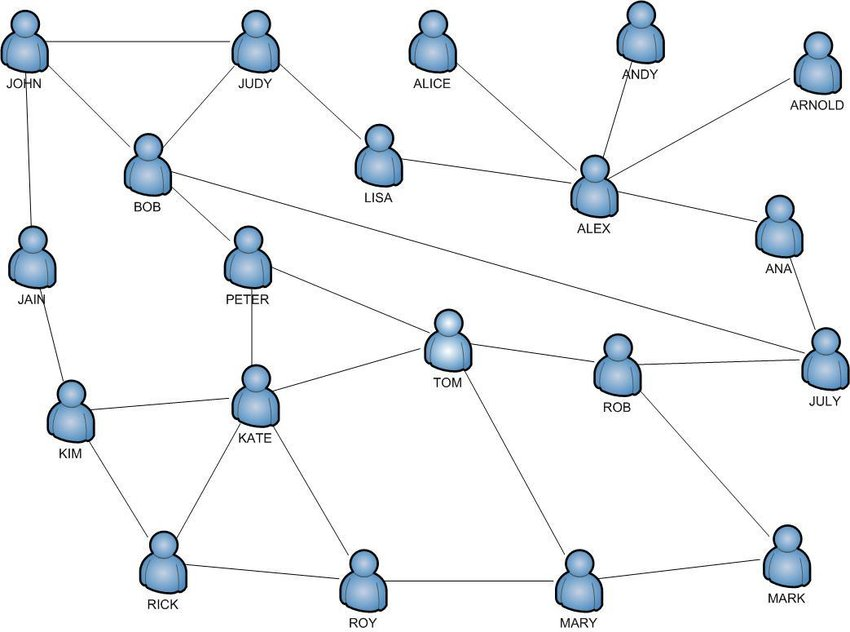
\includegraphics[scale=0.3]{images/Chapter2/friends-graph.png}
        \subcaption{Sơ đồ quan hệ.}
    \end{subfigure}
    \hspace{15mm}
    \begin{subfigure}[b]{0.4\textwidth}
        \centering
        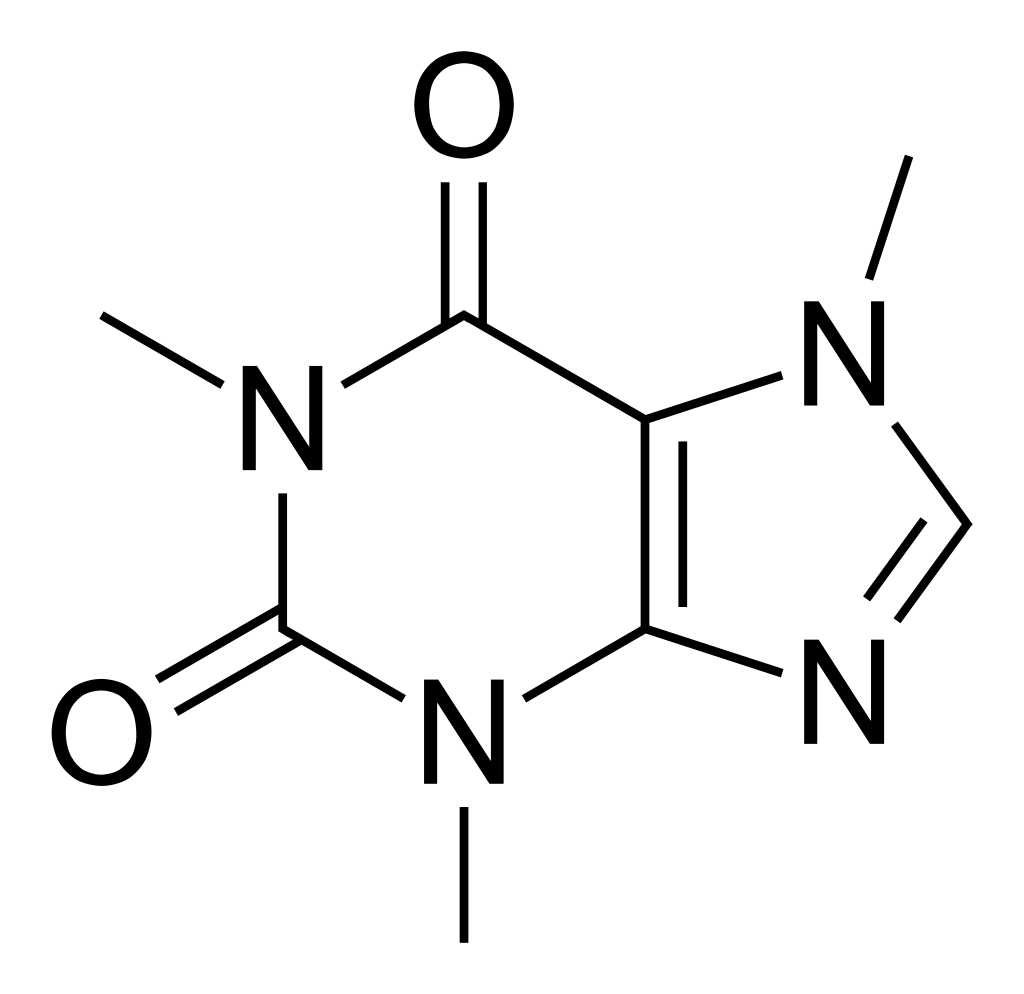
\includegraphics[scale=0.1]{images/Chapter2/caffeine_structure.png}
        \vspace*{8mm}
        \subcaption{Cấu trúc phân tử của caffeine.}
    \end{subfigure}
    \caption{Ví dụ về cấu trúc đồ thị trong thực tế.}
\end{figure}


\subsection{Các loại đồ thị}

\noindent Như đã nói, dữ liệu dạng đồ thị cũng có thể được biểu diễn dưới nhiều dạng khác nhau, khi thiết kế một mạng học sâu để giải quyết một bài toán dạng đồ thị thì cũng nên tìm hiểu kĩ và áp dụng kiểu đồ thị cho phù hợp với bài toán đó. Thông thường thì các model học trên đồ thị sẽ được thiết kế dựa trên tính liên kết có sẵn của dữ liệu rời rạc (VD. Dữ liệu cấu trúc như cấu trúc phân tử, đồ thị tri thức,...) hoặc bằng cách trìu tượng hóa dữ liệu chưa có cấu trúc nhất định (VD. Dữ liệu dạng văn bản trong đoạn văn,...). Theo thống kê của Zhou và đồng nghiệp \cite{review:GNN}, một đồ thị có thể được phân loại như sau:

\begin{itemize}
    \item \textbf{Directed/undirected graph (có hướng/vô hướng):} Như đã định nghĩa ở trên, đồ thị có hướng có nghĩa là thứ tự vào ra của cạnh là một thông tin mà đồ thị vô hướng không có, điều này có thể biểu diễn tính một chiều khi di chuyển từ node này sang node khác, ví dụ là với đường một chiều trong bản đồ giao thông; ngược lại, đồ thị vô hướng trong nhiều trường hợp lại phù hợp hơn cho việc tổng quát hóa vì mỗi cạnh của đồ thị vô hướng có thể hiểu là 2 cạnh có hướng ngược nhau.
    
    \item \textbf{Homogeneous/heterogeneous graph (đồng nhất/không đồng nhất):} Trong đồ thị đồng nhất, chỉ có 1 loại (type) node và cạnh; trong đồ thị không đồng nhất thì có thể có nhiều hơn 1 loại node và cạnh.
    
    \item \textbf{Static/Dynamic graph (tĩnh/động):} Đồ thị tĩnh có cấu trúc/đặc trưng không thay đổi theo thời gian và đồ thị động có cấu trúc/đặc trưng thay đổi theo thời gian.
\end{itemize}

\subsection{Thiết kế chung của mạng GNN} \label{2.2.3-GNN-design}
% [Graph neural networks: A review of methods and applications -- www.sciencedirect.com/science/article/pii/S2666651021000012]
% [A Comprehensive Survey on Graph Neural Networks -- ieeexplore.ieee.org/ielaam/5962385/9312808/9046288-aam.pdf]
% [Strategies for pre-training graph neural networks -- https://arxiv.org/pdf/1905.12265.pdf]
% [Data Augmentation for Deep Graph Learning: A Survey -- https://arxiv.org/pdf/2202.08235.pdf]
% [Weisfeiler and Leman Go Neural: Higher-Order Graph Neural Networks -- https://ojs.aaai.org/index.php/AAAI/article/download/4384/4262]
% [Neural Message Passing for Quantum Chemistry -- http://proceedings.mlr.press/v70/gilmer17a/gilmer17a.pdf]
\subsubsection{Xác định output}
\noindent Khi thiết kế mạng GNN thì ta cần phải xác định được tác vụ (task) của nó. Thông thường khi giải quyết bài toán học trên đồ thị thì có 3 loại tác vụ chính \cite{review:GNN, survey:GNN, survey:aug-for-dgl}:
\begin{itemize}
    \item \textbf{Node-level}: Là các tác vụ tập trung vào dự đoán các đặc trưng của node, ví dụ như phân lớp node, hồi quy, phân cụm...
    
    \item \textbf{Edge-level}: Là các tác vụ dự đoán các đặc trưng của cách cạnh như phân lớp và dự đoán liên kết giữa các node.
    
    \item \textbf{Graph-level}: Là các tác vụ dự đoán các đặc trưng của toàn bộ đồ thị như phân lớp, hồi quy và matching các đồ thị.
\end{itemize}
Tùy vào loại tác vụ nhất định, ta có thể thiết kế 1 hàm mất mát phù hợp. Ví dụ tác vụ phân lớp thì có thể dùng cross-entropy...

\subsubsection{Học biểu diễn} \label{2.2.2-reprensentation-learning}
\noindent Để sử dụng đồ thị trong các ứng dụng khai thác dữ liệu và học máy trong các tác vụ học và dự đoán, đồ thị và các thực thể của nó như nút và cạnh cần được biểu diễn bằng các đặc trưng dạng số. Một trong những cách phổ biến là biểu diễn đồ thị bằng ma trận kề. Tuy nhiên, việc biểu diễn ma trận kề lại tốn khá nhiều bộ nhớ, đặc biệt là với các đồ thị lớn. Một tiếp cận thay thế là trích xuất đặc trưng, ví dụ dựa vào các đặc điểm như bậc (degree), hệ số phân cụm (clustering coefficient), kernel functions,... Tuy nhiên điều này khá hạn chế về mặt thời gian và khó để bắt kịp các tiến trình học. Học biểu diễn (Representation learning) \cite{survey:graph-rep-learning} là giải pháp cho vấn đề vừa nêu trên bằng cách tự động sinh ra các vector biểu diễn cho đồ thị.

% A Survey on Graph Representation Learning Methods (SHIMA KHOSHRAFTAR and AIJUN AN, Electrical Engineering and Computer Science Department, York University, Canada)

\begin{figure} [H]
    \centering
    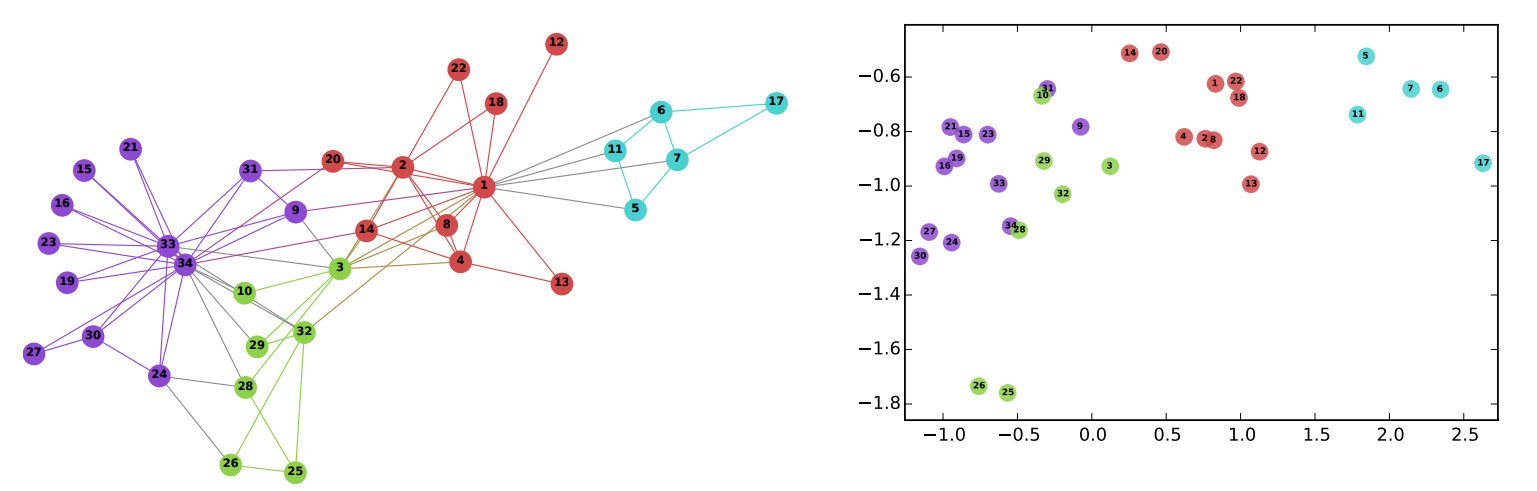
\includegraphics[scale=0.35]{images/Chapter2/node-embedding.png}
    \caption[Ví dụ về node embedding.]{Ví dụ về node embedding. Bên trái là đồ thị gốc, bên phải là biểu diễn của đồ thị trong không gian embedding (Hình ảnh trích từ bài báo của Khoshraftar \cite{survey:graph-rep-learning}).}
    \label{fig:node-embed-example}
\end{figure}

Ý tưởng của \textbf{học biểu diễn} là nhúng một phần hoặc cả đồ thị vào một không gian vector. Mối quan hệ hình học trong không gian này vẫn thể hiện được cấu trúc của đồ thị gốc. Hình \ref{fig:node-embed-example} là một ví dụ về node embedding. Điểm tương đồng giữa các vector embedding của các node cũng thể hiện được sự tương đồng giữa các node trong đồ thị. Điều này cũng đúng với mối liên hệ giữa các cạnh hay là mối liên hệ giữa các đồ thị con trong đồ thị gốc. Giờ đây, các embedding này có thể được sử dụng để làm input cho các tác vụ downstream.

\subsubsection{Quá trình tích chập trên đồ thị -- Neighborhood aggregation/Message passing}

\begin{figure}[H]
    \centering
    \scalebox{.9}{
        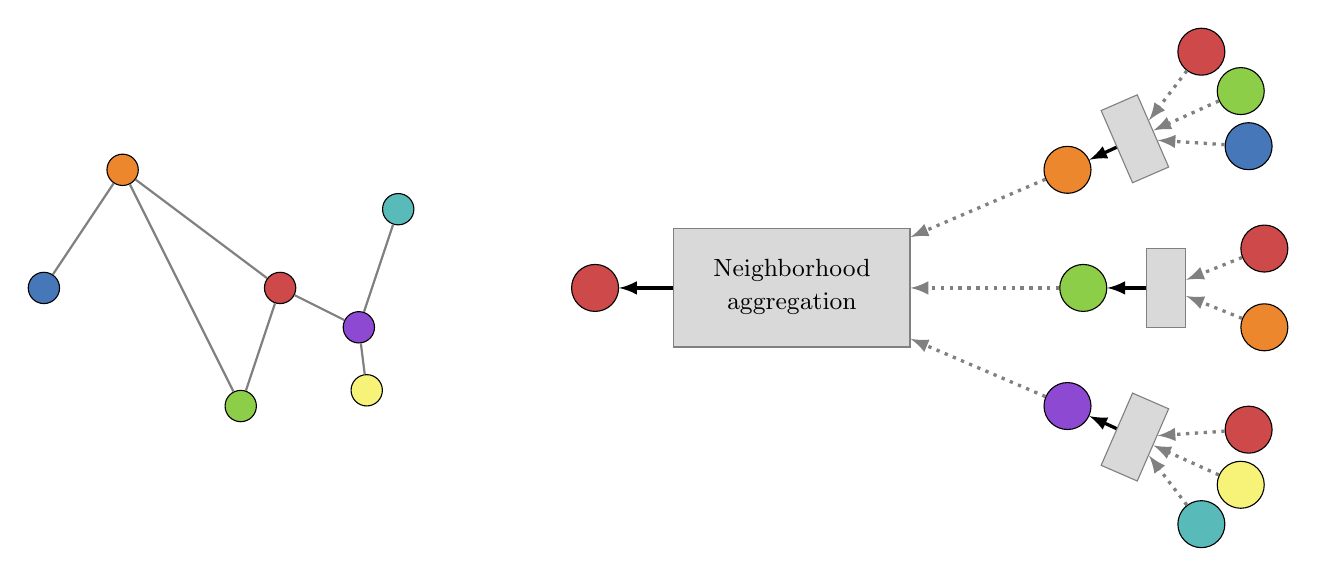
\begin{tikzpicture}[
            vertex/.style = {circle, draw, inner sep=4pt, fill=white},
            red/.style = {vertex, fill=fireenginered},
            orange/.style = {vertex, fill=cadmiumorange},
            blue/.style = {vertex, fill=airforceblue},
            green/.style = {vertex, fill=asparagus},
            purple/.style = {vertex, fill=darklavender},
            cyan/.style = {vertex, fill=electriccyan!80!black},
            yellow/.style = {vertex, fill=goldenyellow},
            ]
            \node[red]      (A) at (5, 1.5) {};
            \node[orange]   (B) at (3, 3) {};
            \node[blue]     (C) at (2, 1.5) {};
            \node[green]    (D) at (4.5, 0) {};
            \node[purple]   (E) at (6, 1) {};
            \node[cyan]     (F) at (6.5, 2.5) {};
            \node[yellow]   (G) at (6.1, 0.2) {};
    
            \node[red, inner sep=6pt]       (A1) at (9, 1.5) {};
            \node[orange, inner sep=6pt]    (B1) at (15, 3) {};
            \node[green, inner sep=6pt]     (D1) at (15.2, 1.5) {};
            \node[purple, inner sep=6pt]    (E1) at (15, 0) {};
            
            \node[draw=gray, fill=gray!30, fit={(10, 0.75) (13, 2.25)}, inner sep=0pt, text height=0.6cm] (NA) {\small Neighborhood\\aggregation};
            
            \node[draw=gray, fill=gray!30, fit={(16, 1) (16.5, 2)}, inner sep=0pt, rotate around={23.5:(-4.75, 0)}] (NA1) {};
            \node[draw=gray, fill=gray!30, fit={(16, 1) (16.5, 2)}, inner sep=0pt] (NA2) {};
            \node[draw=gray, fill=gray!30, fit={(16, 1) (16.5, 2)}, inner sep=0pt, rotate around={-23.5:(-4.75, 0)}] (NA3) {};
    
            \node[red, inner sep=6pt]       (A2) at (16.7, 4.5) {};
            \node[blue, inner sep=6pt]      (C2) at (17.3, 3.3) {};
            \node[green, inner sep=6pt]     (D2) at (17.2, 4) {};
    
            \node[red, inner sep=6pt]       (A3) at (17.5, 2) {};
            \node[orange, inner sep=6pt]    (B3) at (17.5, 1) {};
    
            \node[red, inner sep=6pt]       (A4) at (17.3, -0.3) {};
            \node[cyan, inner sep=6pt]      (F4) at (16.7, -1.5) {};
            \node[yellow, inner sep=6pt]    (G4) at (17.2, -1) {};
            
            \draw[gray, thick]
                (A) -- (B)
                (B) -- (C)
                (A) -- (D)
                (B) -- (D)
                (A) -- (E)
                (E) -- (F)
                (E) -- (G);
    
            \draw[draw, very thick, -latex] (NA) -- (A1);
            \draw[gray, very thick, dotted, -latex] (B1) -- (NA);
            \draw[gray, very thick, dotted, -latex] (D1) -- (NA);
            \draw[gray, very thick, dotted, -latex] (E1) -- (NA);
            \draw[draw, very thick, -latex] (NA1) -- (B1);
            \draw[gray, very thick, dotted, -latex] (A2) -- (NA1);
            \draw[gray, very thick, dotted, -latex] (C2) -- (NA1);
            \draw[gray, very thick, dotted, -latex] (D2) -- (NA1);
            \draw[draw, very thick, -latex] (NA2) -- (D1);
            \draw[gray, very thick, dotted, -latex] (A3) -- (NA2);
            \draw[gray, very thick, dotted, -latex] (B3) -- (NA2);
            \draw[draw, very thick, -latex] (NA3) -- (E1);
            \draw[gray, very thick, dotted, -latex] (A4) -- (NA3);
            \draw[gray, very thick, dotted, -latex] (F4) -- (NA3);
            \draw[gray, very thick, dotted, -latex] (G4) -- (NA3);
            
        \end{tikzpicture}
    }
    \caption{Ví dụ về quá trình tích chập trên đồ thị}
\end{figure}

\noindent Ta có $G = (V, E)$ là đồ thị với tập node $V$ và tập cạnh $E$, $\mathbf{e}_v^{(0)}$ là embedding ban đầu của node $v \in V$, $\mathbf{h}_{uv}$ là embedding của cạnh $(u, v) \in E$, và $\mathcal{N}_v$ là tập các node có cạnh nối với $v$.

Tương tự như một model CNN, trong đó giá trị tích chập của một phần tử trong tensor ở một lớp (layer) là tổ hợp tuyến tính của một nhóm phần tử lân cận với phần tử đó từ lớp trước, một model GNN cơ bản cũng có một mô hình tích chập riêng gọi là Neighborhood aggregation (tổng hợp láng giềng), hay có một tên khác là Message passing (truyền tin) \cite{messagepassing-quantum-chemistry}, trong đó, embedding của node $v$ sẽ được cập nhật (combine) thông qua embedding tổng hợp của các node $u$ nối với $v$ thông qua cạnh $(u, v)$ sử dụng một hàm tổng hợp (aggregate). GC \cite{GC-model}, GG-NN \cite{GG-NN}, GraphSAGE \cite{GraphSAGE} là một số model GNN đời đầu áp dụng phương pháp này.

Thông thường thì phép tích chập này tại lớp thứ $l$ của GNN có biểu diễn toán học \cite{review:GNN, survey:aug-for-dgl, strat-pretrain-GNN, higher-order-GNN} như sau:
\begin{equation}
    \mathbf{e}_v^{(l)} = f_{\text{combine}}^{(l)}(\mathbf{e}_v^{(l-1)}, f_{\text{aggregate}}^{(l)}(\{(\mathbf{e}_v^{(l-1)}, \mathbf{e}_u^{(l-1)}, \mathbf{h}_{uv}) | u \in \mathcal{N}_v\})),
\end{equation}
trong đó, $f_{\text{aggregate}}^{(l)}(\cdot)$ là hàm tổng hợp các node và cạnh lân cận, và có một số lựa chọn như là Mean, Weighted sum \cite{GIN}, LSTM \cite{GraphSAGE}. $f_{\text{combine}}^{(l)}(\cdot)$ là hàm cập nhật embedding của node tại lớp thứ $l$, một lựa chọn phổ biến được để xuất bởi Hamilton và cộng sự \cite{GraphSAGE} là một tác vụ concatenation và mapping tuyến tính. Hai hàm này không nhất thiết phải là riêng biệt mà có thể được tích hợp thành một tác vụ cập nhật duy nhất được xây dựng bởi Kipf và Welling \cite{GCN-model} thấy trong model GCN. Dễ thấy là tại vòng lặp thứ $l$ thì embedding của node $v$ đã có thể nắm bắt được đặc trưng/embedding của các node lân cận trong phạm vi $l$ node. Khi đó, embedding cuối cùng của toàn bộ đồ thị có thể được tính như sau:
\begin{equation}
    \mathbf{e}_G = f_{\text{readout}}(\textbf{\textit{Emb}}_G),
\end{equation}
trong đó $f_{\text{readout}}(\cdot)$ là hàm tính embedding cho toàn bộ đồ thị, $\textbf{\textit{Emb}}_G$ là tập embedding của các node trong đồ thị ở cùng một hoặc nhiều lớp $l \in [0, 1,..., L]$ mà có thể liên quan đến tác vụ dự đoán của model, ví dụ lấy embedding của các node ở lớp cuối cùng $L$: $\textbf{\textit{Emb}}_G = \{\mathbf{e}_v^{(L)} | v \in G\}$.


\section{Tăng cường dữ liệu} \label{2.3-data-aug}

\subsection{Tăng cường dữ liệu là gì?}
\noindent Những năm trở lại đây, ta đang chứng kiến giai đoạn phát triển bùng nổ của các mô hình học sâu (Deep Learning model) trong nghiên cứu lẫn cuộc sống hằng ngày. Một trong những thành tựu to lớn được nhiều người biết đến như công cụ ChatGPT trong lĩnh vực xử lý ngôn ngữ tự nhiên, hệ thống giúp xe tự lái liên quan đến thị giác máy tính,... Tuy vậy, một trong những rào cản khi sử dụng các mô hình học sâu để giải quyết các bài toán trên là ta cần một lượng dữ liệu đủ lớn và đủ tốt để huấn luyện mô hình. Các mô hình học sâu hiện nay, có số lượng tham số cực kỳ lớn, điều này đồng nghĩa với việc ta cần phải cung cấp một lượng lớn dữ liệu tương ứng.

Vậy nếu phải đối mặt với vấn đề thiếu dữ liệu thì ta phải làm thế nào? Câu trả lời đơn giản là ta phải thêm. Thêm thôi là chưa đủ, ta còn phải suy nghĩ thêm sao cho hiệu quả, thêm bằng cách nào?

Cách đầu tiên mà ta có thể dễ dàng nghĩ ngay tới và thực hiện được đó là thu thập, lấy thêm dữ liệu. Một vài ví dụ cho việc này là ta có thể gửi khảo sát nhằm tăng thêm dữ liệu trong tập dữ liệu của ta. Ngoài cách đó ra, ta cũng có thể tự mình mua các dữ liệu mà nhiều bên như Agency thu thập được. Tất nhiên các việc vừa kể nó tốn khá nhiều công sức, tiền bạc. Một cách nữa, khả thi hơn và được áp dụng nhiều trong các mô hình học sâu là tăng cường dữ liệu - Data Augmentation. Đây là một phương pháp xử lý, sinh ra dữ liệu dựa trên dữ liệu có sẵn. Lúc này, ta cần suy nghĩ đến phương pháp nào là tốt nhất trong trường hợp của bản thân. Đôi khi, nếu ta tự thu thập dữ liệu, có thể ta không thể kiếm được nhiều dữ liệu đủ tốt và nhiều, với lại cũng không chắc nếu ta đổ thời gian, tiền bạc, công sức vào việc kiếm đủ lượng data cần thiết thì kết quả liệu có tốt như ta mong đợi. Mỗi trường hợp ta sẽ có sự lựa chọn khác nhau và có thể phương pháp đáng tin cậy có thể mang lại một kết quả tốt là tăng cường dữ liệu.

Tăng cường dữ liệu là một kỹ thuật đươc sử dụng khi có một tập dữ liệu hạn chế và muốn tăng lượng dữ liệu huấn luyện lên dựa vào dữ liệu đã có. Các kỹ thuật tăng cường áp dụng được trên nhiều loại dữ liệu như văn bản, hình ảnh, âm thanh,... Ví dụ đối với bài toán xử lý hình ảnh, với một mẫu dữ liệu, bằng một cách nào đó, ví dụ như xoay ảnh hay là sử dụng mạng GAN để sinh ra ảnh, một ảnh mới có thể được tạo ra, đủ khả năng làm đầu vào của mô hình học \cite{effectiveness-data-aug}. Khi áp dụng phương pháp này, ta có thể giải quyết được vấn đề thiếu dữ liệu của mô hình, đồng nghĩa với việc cải thiện được khả năng dự đoán của mô hình.

\subsection{Một số phương pháp tăng cường dữ liệu phổ biến}
\noindent Phương pháp tăng cường dữ liệu áp dụng được trên cả hình ảnh, văn bản, âm thanh và thậm chí cả đồ thị nữa. Để dễ hình dung, ở phần này, ta sẽ nói qua về việc áp dụng tăng cường dữ liệu áp dụng trên hình ảnh, âm thanh. Còn về việc áp dụng lên đồ thị, là phần chính, nên sẽ được nói chi tiết hơn ở phần sau.

Khi áp dụng tăng cường dữ liệu lên hình ảnh, ta có rất nhiều hướng tiếp cận. Cơ bản nhất, có thể kể đến là xoay ảnh, thay đổi kích thước ảnh, thay đổi màu sắc, độ tương phản, xóa một phần ảnh, thêm nhiễu. Nâng cao hơn là áp dụng mạng GAN vào để sinh ra ảnh \cite{survey:img-aug-for-deeplearning}.

\begin{figure} [H]
    \centering
    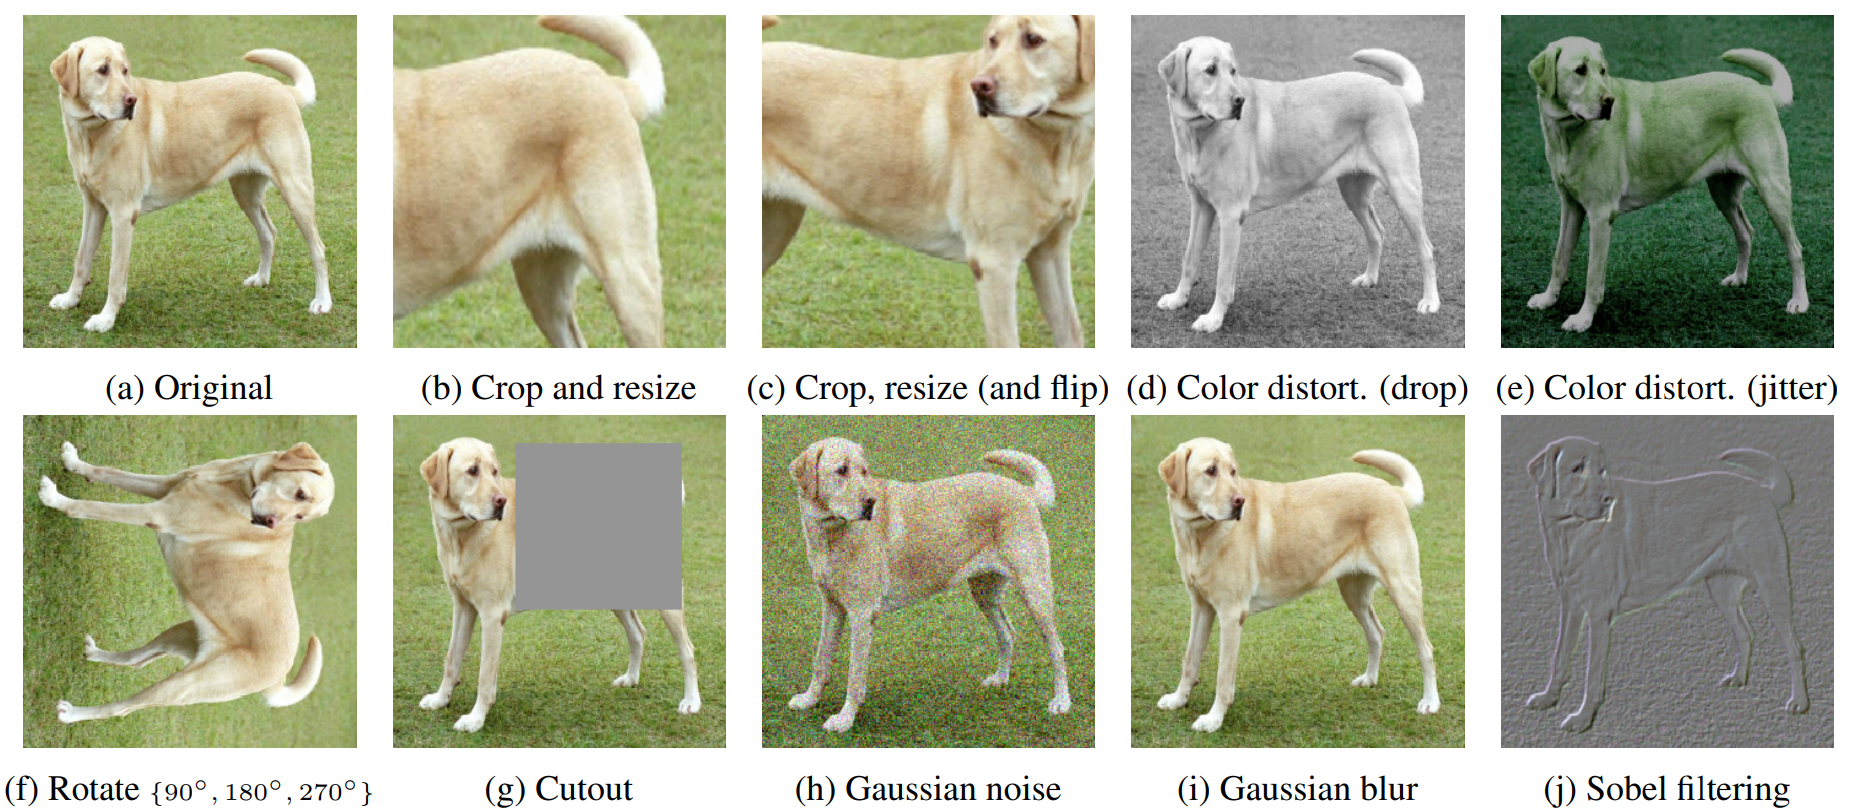
\includegraphics[scale=0.29]{images/Chapter2/example-data-augmentation.png}
    \caption[Ví dụ về việc áp dụng tăng cường dữ liệu lên hình ảnh]{Ví dụ về việc áp dụng tăng cường dữ liệu lên hình ảnh (Hình ảnh trích từ bài báo của Chen \cite{SimCLR}).}
\end{figure}

Việc áp dụng tăng cường dữ liệu lên văn bản cũng rất phổ biến. Ví dụ như thay thế bằng từ đồng nghĩa, xáo trộn câu. COCON \cite{CoCon} -- một kiến trúc mô hình được sử dụng phổ biến cho việc sinh ra dữ liệu dạng văn bản.

Trên đây là những khái niệm cơ bản và một số ví dụ về việc áp dụng phương pháp tăng cường dữ liệu. Ở các phần tiếp theo ta sẽ trình bày cụ thể hơn việc áp dụng tăng cường dữ liệu vào một bài toán cụ thể và việc áp dụng phương pháp này sẽ mang lại hiệu quả như thế nào đối với mô hình.

\section{Học tự giám sát} \label{2.4-ssl}

\noindent Đây sẽ là phần nền tảng cốt lõi nhất cho những thứ ta áp dụng sau này. Học tự giám sát (Self-supervised learning) \cite{ssl-genorcont, ssrl, survey:ssl-for-rec-sys, survey:ssl-from-perspectives, review:ssl-of-GNN} sẽ được sử dụng như là một phương pháp chung để giải quyết các bài toán và có thể áp dụng lên nhiều loại model. Ở phần này, ta sẽ giải thích các khái niệm cơ bản của học tự giám sát, vì sao người ta lại cần đến nó, cấu trúc tổng quát của nó như thế nào. 

\subsection{Học tự giám sát là gì?}

\noindent Việc áp dụng học giám sát để huấn luyện các mô hình học máy đã trở nên rất phổ biến và mang lại nhiều thành tựu to lớn từ trước đến nay. Các mô hình học sâu dần trở nên quá quen thuộc khi nhắc đến như Thị giác máy tính (Computer Vision), Xử lý ngôn ngữ tự nhiên (Natural Language Processing) hay gần đây thì có học đồ thị (Graph Learning). Tuy nhiên, ta nhận ra rằng các mô hình học sâu này luôn trong tình trạng ``đói dữ liệu'', thuật ngữ này đề cập đến vấn đề về kích thước mẫu cần thiết để mô hình học cho ra kết quả với độ chính xác đủ tốt. Với học giám sát, ta cần cung cấp cho mô hình một bộ dữ liệu đầu vào với cặp nhãn đi kèm. Với học không giám sát, ta chỉ cần cung cấp cho mô hình bộ dữ liệu không nhãn, mô hình sẽ học dựa trên cấu trúc của dữ liệu và dự đoán kết quả. Dù có áp dụng phương pháp nào, ta đều nhận thấy rằng khi ta cung cấp cho mô hình học càng nhiều dữ liệu, chất lượng đầu ra của mô hình có thể càng cải thiện. Vậy điều gì sẽ xảy ra khi ta chỉ có một tập dữ liệu có hạn? Lúc đó sẽ dễ dẫn đến trường hợp mô hình thiếu tính tổng quát hóa hay dẫn đến overfitting.

Tuy nhiên, khi xét về vấn đề dữ liệu trong bài toán học giám sát, ta biết rằng để có một bộ dữ liệu được gán nhãn đủ lớn thôi chưa đủ mà còn phải có chất lượng đủ tốt. Đây đã và đang là một vấn đề  còn vướng mắc và gặp rất nhiều hạn chế khi áp dụng trong các bài toán thực tế. Việc gán nhãn cho tập dữ liệu sẽ tốn rất nhiều chi phí, dữ liệu cũng có thể bị mất cân bằng hoặc thậm chí là không thể gán nhãn. Một bài toán nhận được kha khá sự quan tâm dạo thời gian đây với hi vọng giải quyết việc này là học tự giám sát (self-supervised learning). Phương pháp này nổi lên khá nhanh trong thời gian gần đây bởi khả năng áp dụng trên đa dạng loại dữ liệu từ âm thanh, hình ảnh, văn bản và đến cả đồ thị. Học tự giám sát sinh ra với khả năng giải quyết được vấn đề huấn luyện mô hình với phần lớn dữ liệu không được gán nhãn như đã đề cập ở trên. 

Học tự giám sát cho phép quá trình huấn luyện các mô hình học sâu bằng dữ liệu không dãn nhán hoặc một phần nhỏ được gán nhãn. Khi phải đối mặt với bộ dữ liệu không nhãn, học tự giám sát cho phép mô hình học được cách biểu diễn dữ liệu mà không cần gán nhãn dữ liệu bằng chính dữ liệu không nhãn. Khi phải đối mặt với bộ dữ liệu có số lượng nhãn hạn chế, học tự giám sát được áp dụng lên dữ liệu không dán nhãn đóng vai trò như một bước pre-train. Sau đó, sử dụng dữ liệu dán nhãn đã được sử dụng để fine-tune cho pretrain model.

Bên cạnh đó, học tự giám sát có thể  đóng vai là tác vụ phụ, có trách nhiệm bổ trợ cho task chính của mô hình. Áp dụng học tự giám sát không chỉ đạt được hiệu suất tương tự, một số trường hợp lại cho kết quả tốt hơn các mô hình học bởi phương thức có giám sát \cite{review:ssl-of-GNN}.

Mọi người thường nhầm lẫn giữa khái niệm học không giám sát và học tự giám sát. Học tự giám sát có thể được coi là một nhánh của học không giám sát. Vì cả hai đều hoạt động trên dữ liệu không nhãn. Tuy nhiên, học không giám sát chủ yếu hoạt động với các tác vụ phân cụm, gom nhóm, giảm chiều, trong khí đó học tự giám sát lại chủ yếu hoạt động với các tác vụ phân loại, hồi quy như học giám sát \cite{ssl-genorcont}.

Ở phần tiếp theo, ta sẽ giải thích kỹ hơn vì sao học tự giám sát lại quan trọng và được quan tâm trong thời gian gần đây

\subsection{Tại sao cần áp dụng học tự giám sát?} 

\noindent Việc tạo ra một tập dữ liệu tốt với đầy đủ nhãn là rất tốt kém về mặt chi phí lẫn thời gian. Trong khi ta bận tậm đến việc gán nhãn dữ liệu, thì dữ liệu không nhãn lại liên tục được sinh ra. Thay vì đầu tư vào việc gán nhãn, ta có thể tận dụng lượng lớn dữ liệu không nhãn sẵn có. Với học tự giám sát, mô hình có thể học được từ những đặc trưng chính từ bên trong của dữ liệu từ đó cải thiện độ chính xác của mô hình. 

Đi kèm với việc loại bỏ việc gán nhãn thủ công là khả năng mở rộng. Với lượng dữ liệu không nhãn được sinh ra mỗi ngày, dữ liệu sẽ ngày càng một lớn, sẽ rất khó nếu sử dụng các mô hình học giám sát. Thay vì đó, học tự giám sát có thể giải quyết được vấn đề khi không cần để tâm đến việc dữ liệu có nhãn hay không, càng nhiều dữ liệu không nhãn được sinh ra thì càng tốt. Và ắt hẳn điều này cũng giải quyết được việc mất cân bằng dữ liệu.

\subsection{Giới hạn của học tự giám sát?}

\noindent Không phải ngoại lệ, học tự giám sát mang lại nhiều lợi ích và tất nhiên cũng sẽ có một số điều hạn chế đi kèm. Ta cũng cần nắm rõ nhược điểm của học tự giám sát, từ đó tìm cách cải thiện, khắc phục nó.
Học tự giám yêu cầu chi phí sử dụng tài nguyên lớn. Học tự giám sát yêu cầu một lượng lớn dữ liệu, đồng thời cũng yêu cầu một lượng tài nguyên đủ lớn để xử lý được lượng dữ liệu đó. Cụ thể, mô hình cần hiểu được lượng dữ liệu to lớn mà nó được cung cấp, đồng thời tạo ra các nhãn tương ứng. Điều này sẽ tốn rất nhiều thời gian và tài nguyên so với các tác vụ học giám sát vì học tự giám sát được áp dụng khi dữ liệu đã có sẵn nhãn.

Khó giải thích sự hiệu quả mà học tự giám sát mang lại chưa chắc tốt. Mô hình tự học chính bên trong dữ liệu không nhãn mà nó được cung cấp, học được cách biểu diễn dữ liệu, học được các đặc trưng ẩn hữu dụng và ta không thể diễn giải được những điều đấy. Mô hình học tự giám sát sẽ tự động tạo ra các nhãn tương ứng với bộ dữ liệu mà nó được cung cấp mà không có bất kỳ sự hỗ trợ của con người. Điều này làm giảm các tác động dẫn đến lỗi sai của con người. Tuy nhiên, việc này có thể dẫn đến các lỗi sai lớn khi con người không trực tiếp giám sát điều này.

\subsection{Pretext Task and Downstream task}

\noindent Một khái niệm quan trọng trong Học tự giám sát là ``pretext task''.  Thuật ngữ này được dùng ở đây nhằm chỉ ra nhiệm vụ đang giải quyết không phải là vấn đề thật sự mà ta quan tâm, mục đích thực sự của nó là cung cấp cho ta một pre-train model đầy hứa hẹn. Những nhiệm vụ này có thể áp dụng được trên nhiều loại dữ liệu như hình ảnh, âm thanh, tín hiệu nhưng nhìn chung, pretext task có hai đặc điểm phổ biến. Một là mô hình có thể học được các đặc trưng có ích từ việc giải quyết các pretext task. Hai là các tín hiệu giám sát được tạo ra từ chính dữ liệu từ đó giúp mô hình có thể  học được tốt hơn \cite{survey:ssl-from-perspectives}.

Nói rõ hơn, trong học tự giám sát, trước tiên một pretext task sẽ cần được xác định, bên cạnh đó các nhãn giả cũng tự động sinh ra dựa trên một số thuộc tính nhất định của dữ liệu nhằm giúp các thuật toán học học sâu có thể giải quyết các pretext task đó. Sau khi quá trình pretrain này hoàn thành, mô hình học được có thể được sử dụng cho việc giải quyết các downstream task ví dụ như phân loại, phân cụm, phát hiện (cách này còn được gọi là transfer learning)

Hiện nay, có các loại pretext task phổ biến như context-based hay contrastive learning. Với phương thức context-based, có thể lấy việc xoay ảnh, đổi màu, thay đổi vị trí của các phần trong bức ảnh làm ví dụ. Với contrastive learning, ta có thể hiểu đơn giản việc áp dụng nhiệm vụ này có thể khiến các đối tượng gần giống nhau lại gần nhau, các đối tượng khác nhau ngày càng xa nhau trong không gian nhúng. Việc này sẽ nói rõ hơn ở phần dưới.


\chapter{Phương pháp tiếp cận}
\noindent Ở phần này, phương pháp tiếp cận tính được sử dụng trong khóa luận sẽ được trình bày -- bằng cách sử dụng học tự giám sát, ta có thể để giải quyết phần nào vấn đề mà hệ thống gợi ý còn gặp phải. Ở phần trước, ta đã biết khái niệm về Học tự giám sát (Self-supervised Learning), về mạng học sâu đồ thị (Graph Neural Network). Phần này, ta sẽ tập trung tìm hiểu sự liên quan giữa dữ liệu tương tác người dùng -- sản phẩm và dạng biểu diễn đồ thị của dữ liệu đó. Tăng cường dữ liệu (Data Augmentation) đã được trình bày, tuy nhiên chỉ mới đề cập đến hiệu quả của nó trên hình ảnh, ngôn ngữ. Khi áp dụng trên dữ liệu đồ thị, cách thức, hiệu quả của nó mang lại cũng sẽ được trình bày cụ thể hơn, từ đó cho thấy việc áp dụng trên dạng dữ liệu đặc biệt này có gì khác so với dữ liệu dạng hình ảnh, văn bản,.... Sau đó, ta sẽ thảo luận về việc áp dụng Học tự giám sát vào hệ thống gợi ý như thế nào, mang lại hiệu quả như thế nào so với các phương pháp tiếp cận trước.
% 1. Cách áp dụng ssl trên gcn: cách áp dụng data augmentation trên graph --> cách áp dụng self supervised learning (contrastive learning) trên graph
% 2. SSR: có gì khác so vs học sâu graph bth? ssl task loss?? main task loss?? <--> Collaborative filtering + neighborhood aggregation (GCN)??
% 3. Phân tích model

\section{Tăng cường dữ liệu đồ thị} \label{3.1-data-aug}

\noindent Chúng ta đã biết các mô hình học sâu hiện nay luôn trong tình trạng `đói dữ liệu'. Ta càng cung cấp cho mô hình học càng nhiều dữ liệu, chất lượng đầu ra của mô hình có thể càng cải thiện. Nếu thiếu dữ liệu mô hình sẽ thiếu tính tổng quát hóa hoặc có thể dễ bị overfitting. Vậy nên ta rút ra được, có vẻ càng nhiều dữ liệu thì càng tốt, đây sẽ là lúc ta cần áp dụng phương pháp tăng cường dữ liệu nhằm tăng hiệu quả của việc học biểu diễn. Ở phần này, ta sẽ mô tả cụ thể việc tăng cường dữ liệu được áp dụng như thế nào trên dữ liệu dạng đồ thị. Sau khi có được dữ liệu tăng cường, ta sẽ sử dụng chúng ra sao.

Ở chương trước, ta đã biết về kỹ thuật tăng cường dữ liệu (data augmentation) và ứng dụng của nó trên các bài toán Thị giác máy tính (CV) hay Xử lý ngôn ngữ tự nhiên (NLP). Khi áp dụng vào hệ thống gợi ý, ta cần thay đổi về cách thức nhưng nhìn chung về ý tưởng cốt lõi vẫn sẽ giống nhau. Áp dụng cùng cách thức tương tự như trên các bài toán CV hay NLP là bất khả thi \cite{SGL} cho dữ liệu dạng đồ thị vì một vài lí do. Thứ nhất, các đặc trưng của người dùng và sản phẩm là rời rạc, vậy nên các tăng cường trên ảnh như là ngẫu nhiên crop, xoay, hay làm mờ không thể áp dụng được. Thứ hai, data trong CV và NLP là cô lập, trong khi người dùng và sản phẩm trong đồ thị tương tác là có kết nối với nhau và phụ thuộc lẫn nhau.

Khi áp dụng tăng cường dữ liệu, một số cách chọn thay đổi cấu trúc đồ thị, một số khác vẫn giữ nguyên cấu trúc của đồ thị, thay vì đó sẽ xáo trộn nhỏ các đặc trưng của node khiến nó trở nên bất biến với các thuộc tính ban đầu của node \cite{survey:aug-for-dgl, survey:ssl-for-rec-sys}.

% \subsection{Tăng cường cấu trúc đồ thị} \label{3.1.1-graph-structure-aug}
Ở phần này, ta sẽ mô tả các phương pháp phổ biến để tăng cường cấu trúc của đồ thị ban đầu, tức là tăng cường tập node $V$ và tập cạnh $E$. Hiệu quả của nó đã được chứng minh thông qua các model GMAE \cite{GMAE}, MGAE \cite{MGAE}, GraphCL \cite{GraphCL}. Một số phương pháp thường được sử dụng có thể liệt kê như dưới đây.

\begin{itemize}
    \item[] \textbf{Edge/Node Dropout}: với phần trăm tỉ lệ số cạnh muốn xóa/giữ lại, ta có thể  bỏ đi ngẫu nhiên một số cạnh hoặc một số node và các cạnh liên kết với chúng của đồ thị hiện tại nhằm tạo ra các đồ thị mới, bên cạnh đó cũng muốn giữ cấu trúc cơ bản của đồ thị. Ý tưởng này bắt nguồn từ việc chỉ một phần cạnh/node mới đóng góp hữu ích vào việc học biểu diễn và bỏ đi một số kết nối thừa thãi giúp biểu diễn của đồ thị ít bị ảnh hưởng bởi nhiễu. Biểu diễn toán học của đồ thị tăng cường với dropout như sau:
    \vspace*{-8mm}
    \begin{figure}[H]
        \null\hfill
        % 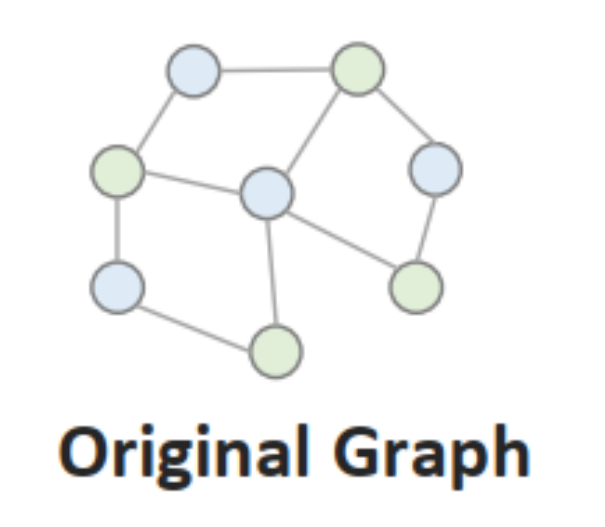
\includegraphics[scale=0.15]{images/Chapter3/original_graph.png}\\
        \begin{subfigure}{0.41\textwidth}
            % \centering
            % 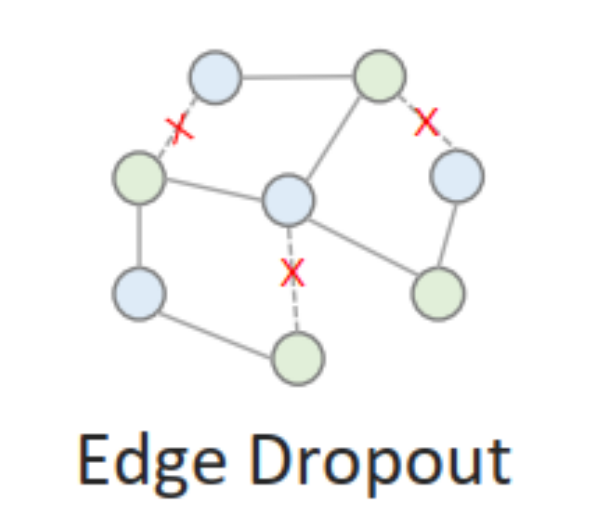
\includegraphics[scale=0.15]{images/Chapter3/edge_dropout.png}
            % \vspace*{-3mm}
            \[
            G_{\text{ED}} = (V, \mathbf{M}_{\text{ED}} \odot E),
            \]
            \caption{Edge dropout augmentation}
        \end{subfigure}
        % \hspace*{+5mm}
        \begin{subfigure}{0.41\textwidth}
            % \centering
            % 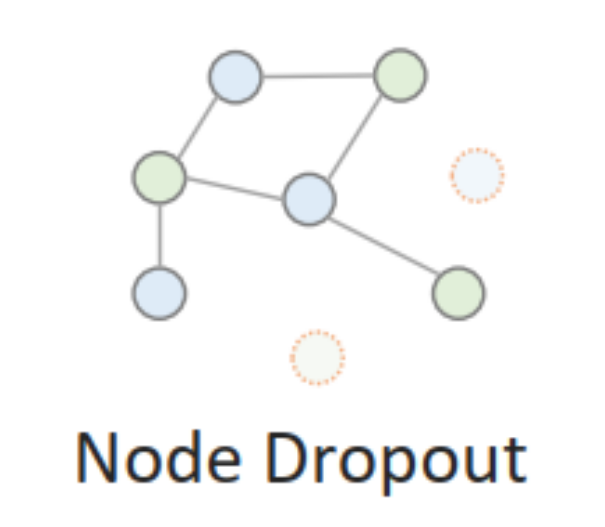
\includegraphics[scale=0.15]{images/Chapter3/node_dropout.png}
            % \vspace*{-3mm}
            \[
            G_{\text{ND}} = (\mathbf{M}_{\text{ND}} \odot V, \mathbf{M}_{\text{ND}}' \odot E),
            \]
            \caption{Node dropout augmentation}
        \end{subfigure}
        \hspace*{+15mm}
        \begin{subfigure}{0\textwidth}
            \begin{equation}\end{equation}
            \vspace*{+7.5mm}
        \end{subfigure}
    \end{figure}
    trong đó, $\mathbf{M}_{\text{ED}} \in \{0, 1\}^{|E|}$ là một masking vector để giúp sinh ra đồ thị tăng cường mà đã bỏ đi một số cạnh; $\mathbf{M}_{\text{ND}} \in \{0, 1\}^{|V|}$ và $\mathbf{M'}_{\text{ND}} \in \{0, 1\}^{|E|}$ là 2 masking vector để sinh ra đồ thị đã được bỏ đi một số node và các cạnh liên kết với các node đó.
    
    \item[] \textbf{Graph Diffusion}: còn được gọi là \textit{Graph rewiring} \cite{graphs-curvature}, phương pháp này tạo ra augmentation dựa trên đặc trưng cấu trúc toàn cục của đồ thị. Cụ thể hơn là \textit{Graph diffusion} thêm cạnh giữa các node có liên kết gián tiếp với nhau thông qua các trọng số đã được tính trước. Biểu diễn toán học của tăng cường diffusion như sau:
    % \begin{center}
    %     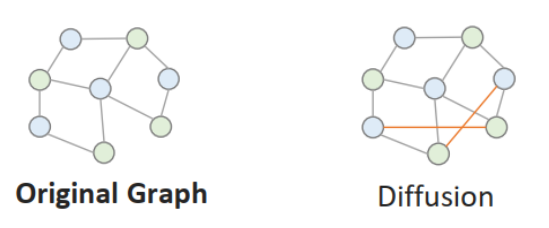
\includegraphics[scale=0.4]{images/Chapter3/graph_diffusion.png}
    % \end{center}
    % \vspace*{-\baselineskip}
    \begin{equation}
        G_{\text{Diff}} = (V, E \cup \tilde{E}),
    \end{equation}
    trong đó $\tilde{E}$ là tập cạnh được thêm vào.

    \item[] \textbf{Node Insertion}: chèn node cũng là một cách thường được sử dụng nhằm mục đích cải thiện Message passing hoặc các liên kết trên đồ thị gốc. Kỹ thuật này thêm các node ảo và các cạnh giữa các node ảo tới các node ban đầu. Biểu diễn toán học của phương pháp tăng cường này như sau:
    \begin{equation}
        G_{\text{NI}} = (V \cup \tilde{V}, E \cup \tilde{E}),
    \end{equation}
    trong đó $\tilde{V}$ và $\tilde{E}$ lần lượt là tập node được thêm và tập cạnh nối giữa $\tilde{V}$ và $V$.

    \item[] \textbf{Subgraph Sampling}: lấy mẫu ngẫu nhiên đồ thị con dựa vào một phần các node và cạnh liên kết của chúng từ đồ thị ban đầu. Phương pháp này khá giống Edge/Node dropout, nhưng thay vì lấy mẫu một cách ngẫu nhiên, đồ thị con mà phương pháp này cho ra thỏa mãn một số tính chất nào đó. Thông thường là sẽ lấy mẫu đồ thị con nhỏ mà bảo tồn càng nhiều thông tin cho việc học càng tốt \cite{data-aug-for-GNN, GNN-via-topo-denoising}. Một lợi thế của phương pháp này là giúp bảo toàn cấu trúc cục bộ trong đồ thị. Biểu diễn toán học của phương pháp tăng cường là:
    % \begin{center}
    %     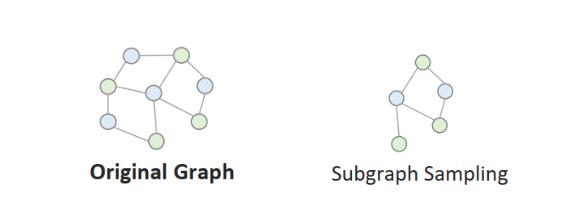
\includegraphics[scale=0.55]{images/Chapter3/subgraph_sampling.png}
    % \end{center}
    % \vspace*{-\baselineskip}
    \begin{equation}
        G_{\text{Sampled}} = (\bm{\mathcal{F}}(V), \bm{\mathcal{F'}}(E)),
    \end{equation}
    trong đó, $\bm{\mathcal{F}}(\cdot)$ và $\bm{\mathcal{F'}}(\cdot)$ lần lượt là hàm lấy mẫu cho các node và cạnh.\\
    Một trong những biến thể phổ biến của Subgraph sampling được áp dụng là \textit{Random walk} \cite{GCC}, từ đồ thị gốc ta chọn một tập node bất kỳ, từ đó lần lượt đi qua các node kề một cách ngẫu nhiên cho đến khi đạt đến số lượng node cần được đi qua cho trước hoặc một đặc tính nào đó đã được thỏa mãn. Nói cách khác là với mỗi node trong tập, ta lấy ra một đồ thị con chứa node đó và các node đã được ``đi qua'', rồi hợp nhất các đồ thị con đó lại.
    \begin{equation}
        G_{RW} = (\mathbf{M}_{RW} \odot V, \mathbf{M}_{RW}' \odot E),
    \end{equation}
    với $\mathbf{M}_{RW}$ là masking vector trích các node đã được chọn và các node được đi qua sau random walk, $\mathbf{M'}_{RW}$ là masking vector trích các cạnh được đi qua.
\end{itemize}


% \subsection{Tăng cường đặc trưng đồ thị}

% \noindent Khác với cách tiếp cận cấu trúc đồ thị, lần này ta sẽ tập trung biến đổi ma trận đặc trưng $\mathbf{X}$. Các phương pháp áp dụng theo hướng tăng cường đặc trưng đồ thị cũng khá phổ biến như các model MGM \cite{MGM}, BGRL \cite{BGRL}.

% \begin{itemize}
%     \item[] \textbf{Feature Corruption}: với phương pháp này, ta sẽ thêm nhiễu vào các đặc trưng của node ban đầu \cite{graph-adversarial-training} hoặc thêm vào biểu diễn đặc trưng đã học \cite{graph-adversarial-SSL}. Biểu diễn toán học của phương pháp corruption này như sau:
%     \[
%     \tilde{x}_i = x_i + c_i,
%     \]
%     trong đó $x_i$ là vector đặc trưng ban đầu hoặc đã học của node $i$, $c_i$ là vector nhiễu.

%     \item[] \textbf{Feature Shuffling}: phương pháp này thay đổi thông tin ngữ cảnh bằng cách đổi hàng và cột trong ma trận đặc trưng $\mathbf{X}$. Biểu diễn toán học là:
%     \[
%     \mathbf{X}_{\text{FS}} = \mathbf{P}_r \mathbf{X} \mathbf{P}_c,
%     \]
%     trong đó, $\mathbf{P}_r \in \{0, 1\}^{n \times n}$ và $\mathbf{P}_c \in \{0, 1\}^{d \times d}$ là ma trận hoán vị cột và dòng, trong 2 ma trận này, mỗi dòng và mỗi cột chỉ chứa duy nhất một giá trị bằng 1.

%     \item[] \textbf{Feature Masking}: bằng cách “che lại” thuộc tính của vài node bằng các mask (một mask được tạo bằng cách lấy sample từ một phân phối chuẩn). Nói dễ hiểu hơn ta sẽ khiến một phần đặc trưng node bằng 0 với một xác suất nào đó. Biểu diễn toán học như sau:
%     \[
%     \mathbf{X}_{\text{FM}} = \mathbf{X} \odot \mathbf{M},
%     \]
%     trong đó $\mathbf{M}$ là ma trận masking với $\mathbf{M}_{ij} = 0$ nếu đặc trưng $j$ của node $i$ bị lược bỏ, $\mathbf{M}_{ij} = 1$ nếu ngược lại.

%     \item[] \textbf{Feature Mixing:} trộn các đặc trưng của node này với các đặc trưng của node khác để tạo ra một node mới. Biểu diễn toán học của việc trộn này như sau:
%     \[
%     \tilde{x} = \alpha x_i + (1 - \alpha) x_j,
%     \]
%     trong đó $\alpha \in [0, 1]$ là hệ số trộn biểu diễn tỉ lệ lấy thông tin giữa $x_i$ và $x_j$.
    
% \end{itemize}

\section{Học trên đồ thị cho hệ thống gợi ý} \label{3.2-graph-learning-recommender}
% 3.2. Học trên đồ thị cho hệ thống gợi ý
% 1. Đồ thị tương tác
% 2. BPR loss
% 3. LightGCN
\subsection{Đồ thị tương tác}
\noindent Để tiện cho phần này, ngoài biểu diễn đồ thị $G$ theo tập node $V$ và cạnh $E$, ta còn có thể biểu diễn nó theo một ma trận kề $\mathbf{A} \in \mathbb{R}^{|V| \times |V|}$ với các giá trị $a_{uv}$ bằng 1 hoặc bằng 0 thể hiện việc có tồn tại cạnh nối giữa hai node $u$ và $v$ hay không. Tức là $\forall u, v \in V, a_{uv} = 1 \Leftrightarrow (u, v) \in E$.

Đối với thông tin phản hồi thu thập được của người dùng, ta có thể chia ra làm 2 loại \cite{CF-for-implicit-feedback} là \textit{Explicit feedback -- phản hồi tường minh} (đánh giá điểm một sản phẩm, viết review, like/dislike...) và \textit{Implicit feedback -- phản hồi ngầm} (click vào trang sản phẩm, hành động mua sản phẩm...). Có thể thấy rằng phản hồi tường minh có lợi thế rất lớn đó là thông tin phản hồi được cung cấp rõ ràng minh bạch, cụ thể hơn, và cho model nhiều thông tin ngữ cảnh hơn; trong khi phản hồi ngầm thì không rành mạch, và không phản ánh đánh giá thực sự của người dùng đối với sản phẩm. Tuy nhiên hầu hết dữ liệu phản hồi của người dùng đối với sản phẩm lại là phản hồi ngầm \cite{denoise-implicit-feedback} vì nhiều lí do như đa số người dùng miễn cưỡng về việc để lại đánh giá/viết review, trong nhiều trường hợp thì việc thu thập dữ liệu tường minh lại còn rất tốn kém về thời gian, tiền bạc và công sức. Cần phải nói thêm là lượng dữ liệu phản hồi này thường là rất lớn, đặc biệt là về lĩnh vực thương mại điện tử \cite{large-scale-amazon-reviews}, do đó, ta sẽ tập trung vào khai thác tập dữ liệu phản hồi ngầm của người dùng, và cũng bỏ qua các mối quan hệ/tương tác giữa người dùng và người dùng, sản phẩm và sản phẩm, cùng với các thuộc tính ban đầu mà các đối tượng đó có thể có (tuổi, giới tính...; loại sản phẩm, kích thước...).

Ta có thể coi dữ liệu phản hồi này như là một đồ thị liên kết giữa người dùng với sản phẩm mà họ đã tương tác, trong đó mỗi node đại diện cho một thực thể người dùng hoặc sản phẩm, và cạnh giữa 2 node người dùng và sản phẩm tồn tại nếu và chỉ nếu người dùng đó đã tương tác với sản phẩm đó. Cụ thể hơn, giả sử ta có tập dữ liệu người dùng $U$ và sản phẩm $I$, cùng với lịch sử tương tác của họ, ta rút ra được đồ thị $G = (V, E)$ mà $V = U \cup I$ là các node và $E = \{(u, i) | u \in U, i \in I\}$ là các cạnh với 2 node $u$, $i$ có tương tác. Lấy ví dụ hình \ref{subfig:interaction-graph}, với $U = \{u_0, u_1, u_2, u_3\}$ và $I = \{i_0, i_1, i_2, i_3, i_4\}$.

\begin{figure}[H]
    \centering
    \begin{subfigure}[b]{0.3\textwidth}
        \centering
        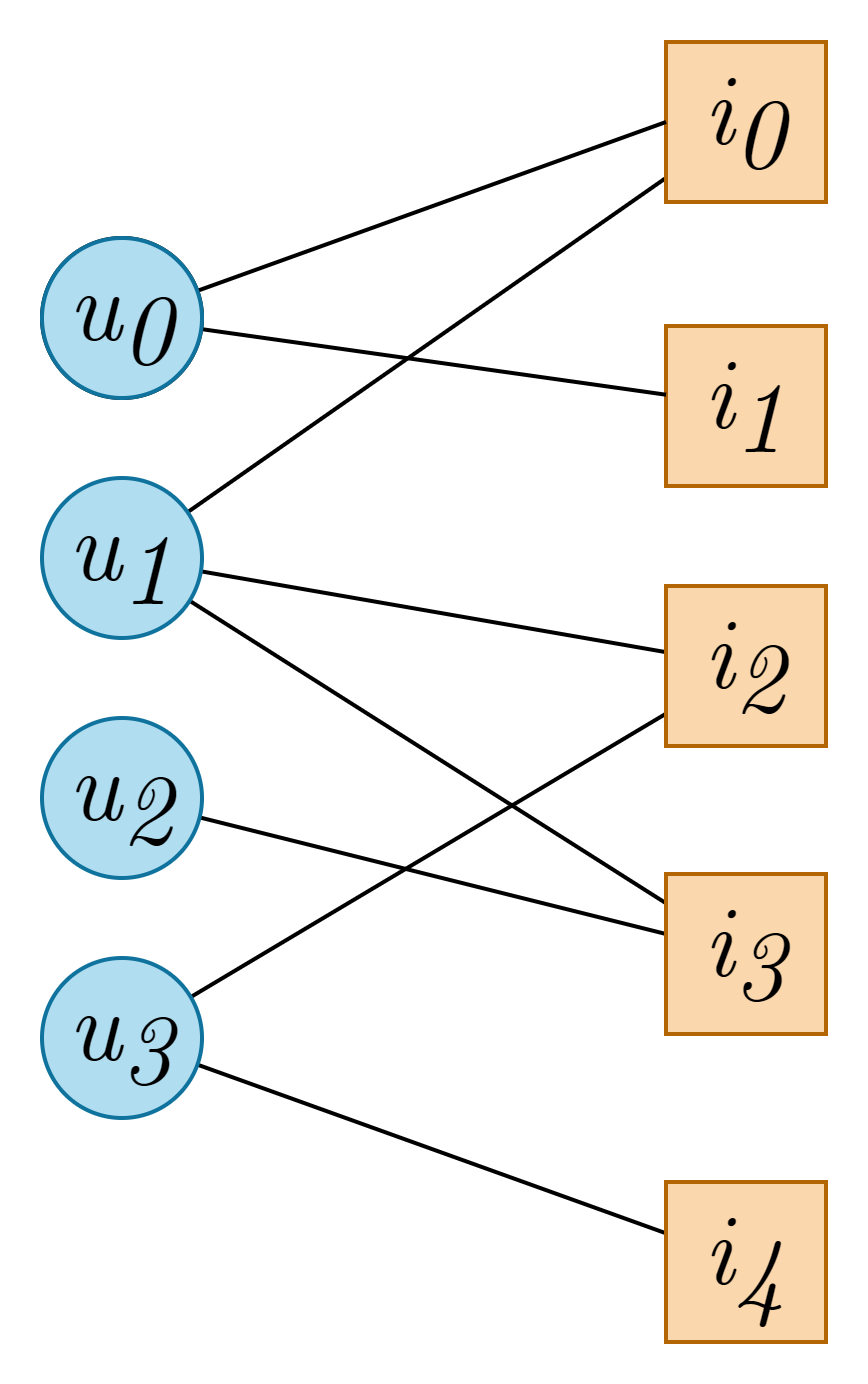
\includegraphics[scale=0.13]{images/Chapter3/user-item_graph.png}
        \subcaption{Đồ thị tương tác.}
        \label{subfig:interaction-graph}
    \end{subfigure}
    \begin{subfigure}[c]{0.12\textwidth}
        \centering
        \vspace*{-65mm}
        \LARGE$\Longleftrightarrow$
    \end{subfigure}
    \begin{subfigure}[b]{0.4\textwidth}
        \centering
        \resizebox{\columnwidth}{!} {
            \centering
            \renewcommand{\arraystretch}{1.2}
            \begin{tabular}{ccc|c|c|c|c|}
                \multicolumn{1}{c}{} & & \multicolumn{5}{c}{Sản phẩm} \\
                \multicolumn{1}{c}{} & \multicolumn{1}{c||}{} &\multicolumn{1}{r|}{$i_0$} & $i_1$ & $i_2$ & $i_3$ & $i_4$ \\
                \hhline{~=::=====}
                \multirow{4}*{\rotatebox[origin=c]{90}{Người dùng}}  
                & \multicolumn{1}{c||}{$u_0$} & \multicolumn{1}{r|}{1} & 1 & 0 & 0 & 0 \\
                \hhline{~-||-----}
                & \multicolumn{1}{c||}{$u_1$} & \multicolumn{1}{r|}{1} & 0 & 1 & 1 & 0 \\
                \hhline{~-||-----}
                & \multicolumn{1}{c||}{$u_2$} & \multicolumn{1}{r|}{0} & 0 & 0 & 1 & 0 \\
                \hhline{~-||-----}
                & \multicolumn{1}{c||}{$u_3$} & \multicolumn{1}{r|}{0} & 0 & 1 & 0 & 1 \\
                \hhline{~-||-----}
            \end{tabular}
        }
        \vspace*{10mm}
        \subcaption{Ma trận tương tác.}
        \label{subfig:interaction-matrix}
    \end{subfigure}
    \caption[Đồ thị và ma trận tương tác.]{Đồ thị tương tác (trái) và ma trận tương tác (phải) giữa người dùng và sản phẩm.}
\end{figure}

\noindent Để biểu diễn dữ liệu đồ thị trên máy tính, ta có thể dùng một ma trận tương tác (hình \ref{subfig:interaction-matrix}) $\mathbf{R} \in \mathbb{R}^{|U|\times|I|}$ trong đó $r_{ui} = 1$ nếu $(u, i) \in E$ và $r_{ui} = 0$ nếu ngược lại. Cuối cùng, một ma trận kề tổng quát của đồ thị có thể được xây dựng như sau:
\begin{equation}
    \mathbf{A} = \begin{pmatrix}
        \mathbf{0} & \mathbf{R} \\
        \mathbf{R}^T & \mathbf{0}
    \end{pmatrix}
    \label{adj-mat-from-R}
\end{equation}

Các giá trị trong ma trận $\mathbf{R}$ đại diện cho lịch sử tương tác và không nhất thiết phải là 0 hoặc 1, một số lớn hơn có thể đại diện cho tần số tương tác và cũng có thể là ngữ cảnh thêm cho hệ thống gợi ý. Để đơn giản hóa, ta sẽ chỉ quan tâm tới việc có tương tác hay không giữa các đối tượng mà không xét đến tần suất tương tác.

Cũng có thể nhận ra là đồ thị tương tác là một đồ thị hai phía -- \textit{Bipartite graph} \cite{bipartite-graph-partition}, đó là đồ thị mà có thể chia tập node $V$ ra làm 2 tập (ví dụ $U$ và $I$) mà không có cạnh nối bất kỳ 2 node nào trong cùng một tập, và có một số đặc điểm có ích cho tác vụ recommendation. Vì đồ thị này được tạo ra từ các tương tác người dùng với sản phẩm nên sẽ chứa tín hiệu Collaborative filtering \cite{MGAT}. Cụ thể là láng giềng liền kề (lịch sử tương tác với sản phẩm đối với node người dùng; hoặc tập các người dùng đã tương tác đối với node sản phẩm) chính là mô tả của node đó và có thể xem là đặc trưng của node. Láng giềng ở bước nhảy thứ 2 mô tả những người dùng/sản phẩm tương tự.
% Với tính chất của dữ liệu tương tác, ta có thể nói ma trận kề $\mathbf{A}$ và ma trận đặc trưng $\mathbf{X}$ của đồ thị tương tác (đã nhắc đến ở đầu phần \ref{3.1.1-graph-structure-aug}) là một.

\subsection{Bayesian Personalized Ranking loss}
\noindent \textbf{Bayesian Personalized Ranking (BPR)} \cite{BPR-loss} là một phương pháp để tối ưu hóa tham số của một model gợi ý dự đoán ranking (đánh giá) của người dùng về một sản phẩm dựa trên dữ liệu tương tác ngầm của người dùng.

Ta sẽ phân tích kỹ ma trận tương tác $\mathbf{R}$. Nhắc lại, $r_{ui} = 1$ có nghĩa là có tương tác giữa người dùng $u$ và sản phẩm $i$, giả sử là tương tác ``người dùng mua sản phẩm'', $r_{ui} = 0$ có nghĩa là không có tương tác. Điểm đặc biệt của phản hồi ngầm là khi có tương tác giữa người dùng và sản phẩm thì có khả năng rất cao là, và sẽ được coi như là, tương tác ``tích cực'' \cite{BPR-loss} (người dùng thích sản phẩm, đánh giá cao...). Đáng lẽ là khi thu thập dữ liệu thì ta có thêm một giá trị âm cho $r_{ui}$ để đại diện cho tương tác ``tiêu cực'' (người dùng không thích sản phẩm). Tuy nhiên trong thực tế thì những tương tác tiêu cực đó hầu như không có. Một giải thích đơn giản là khi người dùng mua sản phẩm thì thường là họ đã biết trước họ sẽ mua cái gì rồi. Những cặp người dùng -- sản phẩm không có tương tác thì một là do người dùng thực sự không thích sản phẩm, hai là dữ liệu bị thiếu/không rõ ràng (họ đang để dành tiền, họ chưa bao giờ thấy sản phẩm đó nhưng có khả năng sẽ thích nó...). Như vậy giá trị ma trận \ref{subfig:interaction-matrix} có thể hiểu như ma trận \ref{subfig:raw-data} ở ví dụ sau:

\begin{figure}[H]
    \centering
    \begin{subfigure}[c]{0.4\textwidth}
        \centering
        \resizebox{\columnwidth}{!} {
            \centering
            \renewcommand{\arraystretch}{1.2}
            \begin{tabular}{cc|c|c|c|c|}
                \multicolumn{1}{c||}{} &\multicolumn{1}{r|}{$i_0$} & $i_1$ & $i_2$ & $i_3$ & $i_4$ \\
                \hhline{=::=====}
                \multicolumn{1}{c||}{$u_0$} & \multicolumn{1}{r|}{+} & + & \textcolor{orange}{\textbf{?}} & \textcolor{orange}{\textbf{?}} & \textcolor{orange}{\textbf{?}} \\
                \hhline{-||-----}
                \multicolumn{1}{c||}{$u_1$} & \multicolumn{1}{r|}{+} & \textcolor{orange}{\textbf{?}} & + & + & \textcolor{orange}{\textbf{?}} \\
                \hhline{-||-----}
                \multicolumn{1}{c||}{$u_2$} & \multicolumn{1}{r|}{\textcolor{orange}{\textbf{?}}} & \textcolor{orange}{\textbf{?}} & \textcolor{orange}{\textbf{?}} & + & \textcolor{orange}{\textbf{?}} \\
                \hhline{-||-----}
                \multicolumn{1}{c||}{$u_3$} & \multicolumn{1}{r|}{\textcolor{orange}{\textbf{?}}} & \textcolor{orange}{\textbf{?}} & + & \textcolor{orange}{\textbf{?}} & + \\
                \hhline{-||-----}
            \end{tabular}
        }
        \subcaption{Dữ liệu mà $\mathbf{R}$ diễn tả.}
        \label{subfig:raw-data}
    \end{subfigure}
    \begin{subfigure}[c]{0.15\textwidth}
        \centering
        \Large$\dashrightarrow$
    \end{subfigure}
    \begin{subfigure}[c]{0.4\textwidth}
        \centering
        \resizebox{\columnwidth}{!} {
            \centering
            \renewcommand{\arraystretch}{1.2}
            \begin{tabular}{cc|c|c|c|c|}
                \multicolumn{1}{c||}{} &\multicolumn{1}{r|}{$i_0$} & $i_1$ & $i_2$ & $i_3$ & $i_4$ \\
                \hhline{=::=====}
                \multicolumn{1}{c||}{$u_0$} & \multicolumn{1}{r|}{+} & + & \textcolor{orange}{+} & \textcolor{orange}{+} & \textcolor{orange}{--} \\
                \hhline{-||-----}
                \multicolumn{1}{c||}{$u_1$} & \multicolumn{1}{r|}{+} & \textcolor{orange}{--} & + & + & \textcolor{orange}{+} \\
                \hhline{-||-----}
                \multicolumn{1}{c||}{$u_2$} & \multicolumn{1}{r|}{\textcolor{orange}{--}} & \textcolor{orange}{--} & \textcolor{orange}{+} & + & \textcolor{orange}{--} \\
                \hhline{-||-----}
                \multicolumn{1}{c||}{$u_3$} & \multicolumn{1}{r|}{\textcolor{orange}{+}} & \textcolor{orange}{--} & + & \textcolor{orange}{--} & + \\
                \hhline{-||-----}
            \end{tabular}
        }
        \subcaption{Dữ liệu tương tác có thể có.}
    \end{subfigure}
    \caption[Dữ liệu diễn tả tương tác ngầm.]{Dữ liệu diễn tả tương tác ngầm và thiếu (trái), và dữ liệu có thể có (phải).}
    \label{subfig:interpreted-matrix}
\end{figure}

\noindent trong đó, dấu $+$ biểu diễn tương tác tích cực, $-$ biểu diễn tương tác tiêu cực, và \textcolor{orange}{\textbf{?}} là giá trị thiếu.

Tuy là dữ liệu có giá trị thiếu và ma trận $\mathbf{R}$ chỉ biểu diễn tương tác, ta sẽ coi việc ``người dùng $u$ tương tác với sản phẩm $i$ mà không có tương tác với sản phẩm $j$'' đồng nghĩa với việc ``$u$ ưa thích $i$ hơn $j$'', tức là $r_{ui} = 1$ và $r_{uj} = 0$. Ngoài ra, những cặp sản phẩm $(i, j)$ mà $r_{ui} = r_{uj}$ ngụ ý là mức độ ưa thích của $u$ với $i$ và $j$ là như nhau hoặc không thể kết luận được. Xét cho cùng thì dự đoán một giá trị tương tác tích cực hay một giá trị tiêu cực là rất khó nếu dữ liệu tương tác có dạng như trên. Thay vì đó, ta sẽ dự đoán xem người dùng sẽ xếp thứ hạng (rank) những sản phẩm trong tập sản phẩm như thế nào.

Rendle và các cộng sự \cite{BPR-loss} định nghĩa một quan hệ toán học $>_u \in I^2$ mang ý nghĩa so sánh mức độ yêu thích của người dùng trên tập sản phẩm $I$. Đó là khi ta nói \(i >_u j\; (i, j \in I)\) thì có nghĩa là người dùng $u$ thích sản phẩm $i$ hơn sản phẩm $j$. Quan hệ này mang tính chất thứ tự toàn phần, cụ thể:
\begin{align*}
    & \forall i, j \in I: i \neq j \implies i >_u j \lor j >_u i \tag{toàn phần} \\
    & \forall i, j \in I: i >_u j \land j >_u i \implies i = j \tag{phi đối xứng} \\
    & \forall i, j, k \in I: i >_u j \land j >_u k \implies i >_u k \tag{bắc cầu}
\end{align*}
Để tiện hơn, ta cũng định nghĩa:
\begin{equation}
    \begin{aligned}
        I_u^+ & = \{i \in I \; | \; (u, i) \in E\}, \\
        U_i^+ & = \{u \in U \; | \; (u, i) \in E\}, \\
        D & = \{(u, i, j) \; | \; i \in I_u^+ \land j \in I \setminus I_u^+\},
    \end{aligned}
\end{equation}
trong đó, $I_u^+$ là tập các sản phẩm mà người dùng $u$ tương tác, $U_i^+$ là tập các người dùng có tương tác với sản phẩm $i$, $D$ là tập các bộ ba $(u, i, j)$ đại diện cho người dùng $u$ thích sản phẩm $i$ hơn $j$. Ngoài ra, $D$ còn sẽ đại diện cho dữ liệu huấn luyện. Rendle và công sự đưa ra 2 ưu điểm \cite{BPR-loss} của cách tiếp cận này:
\begin{itemize}
    \item[1.] Dữ liệu huấn luyện bao gồm các tương tác tích cực, tiêu cực và dữ liệu bị thiếu. Hai sản phẩm thiếu dữ liệu tương tác của người dùng sẽ là hai sản phẩm mà ta cần phải dự đoán cái nào được đánh thứ hạng cao hơn. Vì vậy, xét theo cặp sản phẩm thì tập huấn luyện $D$ và tập test thử nghiệm là rời nhau.

    \item[2.] Dữ liệu huấn luyện có duy nhất một mục đích là để giúp huấn luyện dự đoán ranking.
\end{itemize}

Giả sử ta có tập tham số $\Theta$ (một vector nhiều chiều) của một model gợi ý bất kỳ. Để tìm đúng ranking cá nhân cho các sản phẩm, công thức BPR nhắm tìm giá trị cho $\Theta$ để tối đại hóa xác suất hậu nghiệm sau:
\begin{equation}
    p(\Theta | >_u) \propto p(>_u | \Theta) p(\Theta),
\end{equation}
kí hiệu $>_u$ ở đây là cấu trúc của sự ưa thích đối với người dùng $u$, nói cách khác, kí hiệu đại diện cho ranking cá nhân mong muốn của người dùng $u$ trên tập sản phẩm.

Ta có hai giả định đối với dữ liệu: (i) thứ tự các cặp sản phẩm $(i, j)$ trong quan hệ ưa thích của mỗi người dùng là độc lập với nhau, và (ii) tất cả người dùng hành động độc lập với nhau. Từ giả định (i), ta có thể viết lại hàm likelihood $p(>_u | \Theta)$ cho người dùng $u$ bằng cách triển khai tích xác suất như sau:
\begin{equation}
    p(>_u | \Theta) = \prod_{(i,j) \in I \times I}{p(i >_u j | \Theta)^{\delta((u,i,j) \in D)} \cdot \left(1 - p(i >_u j | \Theta)\right)^{\delta((u,j,i) \notin D)}},
\end{equation}
với $\delta(b)$ bằng 1 nếu mệnh đề $b$ đúng, bằng 0 nếu ngược lại. Giả định (ii) cho thấy rằng xác suất $p$ có thể được kết hợp với tất cả $u \in U$. Cùng với (i), ta có:
\begin{equation}
    \prod_{u \in U}{p(>_u | \Theta)} = \prod_{(u,i,j) \in U \times I \times I}{p(i >_u j | \Theta)^{\delta((u,i,j) \in D)} \cdot \left(1 - p(i >_u j | \Theta)\right)^{\delta((u,j,i) \notin D)}}
    \label{eq:prod-p}
\end{equation}
Nhờ vào tính toàn phần và phi đối xứng, công thức trên có thể được đơn giản hóa như sau:
\begin{equation}
    \prod_{u \in U}{p(>_u | \Theta)} = \prod_{(u,i,j) \in D}{p(i >_u j | \Theta)}
\end{equation}
Tuy nhiên, tới đây vẫn chưa thể lập một thứ tự ranking cho một người dùng được. Để đảm bảo cả 3 tính chất toàn phần, phi đối xứng và bắc cầu của quan hệ $>_u$, Rendle \cite{BPR-loss} định nghĩa xác suất người dùng ưa thích sản phẩm $i$ hơn $j$ như sau:
\begin{equation}
    p(i >_u j | \Theta) = \sigma(\hat{x}_{uij}(\Theta)),
\end{equation}
với $\sigma(x)$ là hàm logistic sigmoid:
\begin{equation}
    \sigma(x) = \frac{1}{1 + e^{-x}}
\end{equation}
Hàm $\hat{x}_{uij}(\Theta)$ là một hàm số thực nhận $\Theta$ là đầu vào, và nắm bắt được mối quan hệ giữa người dùng $u$, sản phẩm $i$ và $j$. Nói cách khác, $\hat{x}_{uij}$ phải thể hiện được mức độ ưa thích của $u$ với $i$ như thế nào so với $j$. Để tiện hơn, ta sẽ bỏ qua tham số $\Theta$ khi viết $\hat{x}_{uij}$ cho các công thức ở sau.

Để hoàn thiện hướng tiếp cận, ta xem $p(\Theta)$ như là phân phối chuẩn với mean bằng 0 và ma trận variance-covariance $\Sigma_{\Theta}$:
\begin{equation}
    p(\Theta) \sim \mathcal{N}(0, \Sigma_{\Theta})
\end{equation}
Để giảm số lượng hyperparameter, ta đặt $\Sigma_{\Theta} = \lambda_{\Theta} \mathbf{I}$, với $\mathbf{I}$ là ma trận đơn vị cùng kích thước với $\Sigma_{\Theta}$. Bài toán tối ưu sẽ quy về tìm cực đại của:
\begin{equation}
    \begin{aligned}
        \text{BPR-Opt} & = \ln{p(\Theta | >_u)} \\
                       & = \ln{(p(>_u | \Theta) p(\Theta))} \\
                       & = \ln{\left(\prod_{(u,i,j) \in D}{\sigma(\hat{x}_{uij})} p(\Theta)\right)} \\
                       & = \sum_{(u,i,j) \in D}{\ln{\sigma(\hat{x}_{uij})}} + \ln{p(\Theta)} \\
                       & = \sum_{(u,i,j) \in D}{\ln{\sigma(\hat{x}_{uij})}} - \lambda_{\Theta} \lVert \Theta \rVert^2,
    \end{aligned}
    \label{eq:bpr-opt}
\end{equation}
trong đó, $\lambda_{\Theta}$ là tham số regularization của model. Vì $i$ được xem như là ``ưa thích hơn'' $j$ đối với $u$, ta có thể chọn một công thức sao cho $\hat{x}_{uij}$ phản ánh được điều đó. Như vậy, ta có thể đơn giản hóa $\hat{x}_{uij}$ như sau:
\begin{equation}
    \hat{x}_{uij} = \hat{y}_{ui} - \hat{y}_{uj},
    \label{eq:xuij-as-yuij}
\end{equation}
trong đó, $\hat{y}_{ui}$ và $\hat{y}_{uj}$ lần lượt là ranking dự đoán của người dùng $u$ đối với $i$ và $j$. Cơ bản là công thức trên cho biết sự khác nhau giữa dự đoán về độ ưa thích với hai sản phẩm $i$ và $j$. Theo công thức \eqref{eq:bpr-opt} và ngữ cảnh là cực đại hóa BPR-Opt, công thức thay thế cho $\hat{x}_{uij}$ ở trên cũng tương tự như là việc ``thúc đẩy'' ranking của $i$ sao cho cao hơn $j$ cho người dùng $u$.

Từ \eqref{eq:bpr-opt} và \eqref{eq:xuij-as-yuij}, ta có hàm mất mát sau cho một model gợi ý:
\begin{equation}
    \begin{aligned}
        \mathcal{L}_{\text{BPR}} & = -\text{BPR-Opt} \\
                                 & = -\sum_{(u,i,j) \in D}{\ln{\sigma(\hat{y}_{ui} - \hat{y}_{uj})}} + \lambda_{\Theta} \lVert \Theta \rVert^2
    \end{aligned}
    \label{eq:bpr-loss}
\end{equation}

\subsection{Áp dụng học đồ thị lên hệ thống gợi ý} \label{3.2.3-GNN-on-rec}

\noindent Về việc học trên đồ thị cho tác vụ gợi ý thì đã tồn tại một số model \cite{PinSAGE, GC-MC, NGCF, LightGCN} được sử dụng khá phổ biến. Trong PinSAGE \cite{PinSAGE}, Ying và các cộng sự xây dựng một framework baseline, học biểu diễn để giúp tăng chất lượng học cho một thuật toán học downstream gợi ý khác; GC-MC \cite{GC-MC} và NGCF \cite{NGCF} là hai trong những model đầu tiên áp dụng học trên đồ thị để khai tác tín hiệu collaborative filtering. Trong khóa luận này, \textbf{LightGCN} \cite{LightGCN}, một model nhẹ và hiệu quả, sẽ được chọn cho việc học và dự đoán gợi ý trên đồ thị tương tác. Cũng cần phải nhắc đến là hướng tiếp cận học đồ thị trong phạm vi khóa luận này là một thuật toán học đặc biệt mà trong đó toàn bộ dữ liệu, cùng với nhau, có cấu trúc/phân phối/đặc trưng của một đồ thị và có nhiệm vụ dự đoán các tính chất của đồ thị hoặc một phần đồ thị đó (\textit{transductive learning}) \cite{GCN-model, DGCN, NGCF}, tức là model không thể đưa ra dự đoán cho bộ dữ liệu với cấu trúc đồ thị khác \cite{review:GNN}. Trái với một loại khác của học đồ thị mà trong đó mỗi mẫu dữ liệu là một đồ thị riêng và model đưa ra dự đoán trên dữ liệu chưa từng thấy (\textit{inductive learning}) \cite{GraphSAGE, PinSAGE, GC-model, GG-NN}. Tuy nhiên khi áp dụng học đồ thị thì ý tưởng và cách học của 2 loại model này là tương tự nhau.

\subsubsection{Mô tả LightGCN}

\noindent Các công trình ứng dụng học mạng tích chập đồ thị cho hệ thống gợi ý trước khi LightGCN ra đời thiếu sự phân tích kỹ lưỡng về cách giảm độ phức tạp của mạng tích chập đồ thị để phù hợp hơn với tác vụ gợi ý, trong khi mạng tích chập đồ thị lại được tạo ra để giải quyết một phạm vi lớn các vấn đề liên quan đến đồ thị và có rất nhiều phép tính trong mạng neuron. Theo tìm hiểu của các tác giả của LightGCN, Xiangnan He và các đồng nghiệp \cite{LightGCN}, hai trong những đặc điểm phổ biến của một mạng học máy đồ thị là biến đổi đặc trưng -- \textit{feature transformation}, và hàm kích hoạt phi tuyến tính -- \textit{nonlinear activation} không những không có tác động đáng kể đến việc khai thác tín hiệu collaborative filtering, mà còn tăng độ phức tạp cho việc huấn luyện và làm giảm chất lượng của dự đoán. Mục tiêu của LightGCN là đơn giản hóa thiết kế chung của mạng tích chập đồ thị, giúp mô hình nhẹ hơn và phù hợp hơn với tác vụ gợi ý.

\subsubsection{Thiết kế tích chập của LightGCN}
\noindent Ta đã đề cập đến kiến trúc chung của mạng học đồ thị ở phần \ref{2.2.3-GNN-design}. Gọi $\mathbf{e}_u^{(l)}$ và $\mathbf{e}_i^{(l)}$ lần lượt là các embedding của người dùng $u$ và sản phẩm $i$ tại lớp thứ $l$; gọi $\mathcal{N}_u$ là tập sản phẩm mà người dùng $u$ tương tác, và $\mathcal{N}_i$ là tập các người dùng có tương tác với sản phẩm $i$. Tác vụ tích chập (Neighborhood aggregation) của LightGCN được định nghĩa như sau:
\begin{equation}
    \begin{aligned}
        \mathbf{e}_u^{(l+1)} & = \sum_{i \in \mathcal{N}_u}{\frac{1}{\sqrt{|\mathcal{N}_u|} \sqrt{|\mathcal{N}_i|}} \mathbf{e}_i^{(l)}}, \\
        \mathbf{e}_i^{(l+1)} & = \sum_{u \in \mathcal{N}_i}{\frac{1}{\sqrt{|\mathcal{N}_i|} \sqrt{|\mathcal{N}_u|}} \mathbf{e}_u^{(l)}},
    \end{aligned}
    \label{lightgcn-neiagg}
\end{equation}
với hệ số bình thường hóa $\frac{1}{\sqrt{|\mathcal{N}_u|} \sqrt{|\mathcal{N}_i|}}$ được lấy từ thiết kế của model GCN \cite{GCN-model}, mục đích của hệ số là làm giảm sự gia tăng nhanh chóng của các giá trị trong vector embedding khi chạy quá trình tích chập qua nhiều lớp. Có một số công thức khác có thể thay thế cho hệ số này, nhưng các tác giả của LightGCN tìm hiểu thấy là cách làm này cũng đủ tốt. Hàm tích chập được chọn của LightGCN chỉ là một hàm tổng có trọng số đơn giản, hoàn toàn không có biến đổi đặc trưng hay kích hoạt phi tuyến gì cả, giúp model nhẹ hơn nhiều.

Để ý kỹ là với mỗi node $u$ hoặc $i$, ta không tổng hợp embedding của chính node đó từ lớp trước mà chỉ tổng hợp các node láng giềng. Lý do là tác vụ tổng hợp các embedding lại để sử dụng cho tác vụ dự đoán (sẽ nói trong phần tiếp theo) có thể nắm bắt việc tổng hợp chính các node đó rồi.

\subsubsection{Kết hợp các embedding cho dự đoán}
\noindent Trong model LightGCN, các tham số học $\Theta$ của model chính là embedding ban đầu của các node, tức là embedding tại lớp thứ 0, $\{\mathbf{e}_u^{(0)} | u \in U\}$ và $\{\mathbf{e}_i^{(0)} | i \in I\}$; các embedding lớp thứ 0 có thể được lấy ngẫu nhiên từ một phân phối nào đó. Sau khi tích chập được $L$ lớp, các embedding cuối cùng của các node sẽ được kết hợp như sau:
\begin{equation}
    \mathbf{e}_u = \sum_{l=0}^{L}{\alpha_l \mathbf{e}_u^{(l)}}, \qquad
    \mathbf{e}_i = \sum_{l=0}^{L}{\alpha_l \mathbf{e}_i^{(l)}},
\end{equation}
trong đó, $\alpha_l \geq 0$ định nghĩa mức độ quan trọng (trọng số) của lớp thứ $l$ và có thể được coi như là hyperparameter hoặc là tham số cho một mạng attention \cite{survey:attention-models, attentive-CF}. Theo thử nghiệm của He và đồng nghiệp \cite{LightGCN}, đặt các giá trị $\alpha_l$ đều bằng $1/(K+1)$ cũng đủ để giúp model đạt hiệu suất tốt, một lý do khác là để giữ tính đơn giản và nhẹ của model.

\noindent Các tác giả của LightGCN đưa ra 3 lý do \cite{LightGCN} tại sao lại chọn tổng hợp các embedding như thế này để đưa vào tác vụ dự đoán:
\begin{itemize}
    \item[(1)] Khi số lớp trong model càng nhiều thì các embedding sẽ chịu nhiều ảnh hưởng của vấn đề ``làm nhẵn'' -- oversmoothing \cite{insights-GCN}, tức là các embedding sẽ bị kéo lại gần nhau, các embedding ở các cụm khác nhau càng trở nên khó phân biệt. Vậy nên nếu chỉ sử dụng lớp cuối cùng để đưa ra dự đoán là rất rắc rối.

    \item[(2)] Các embedding ở mỗi lớp nắm bắt những đặc điểm khác nhau. Ví dụ embedding ở lớp thứ nhất chứa thông tin về những người dùng và sản phẩm có tương tác, embedding ở lớp thứ hai chứa nắm bắt thông tin về những người dùng, sản phẩm tương tự nhau, và các embedding ở lớp cao hơn nắm bắt những đặc điểm bậc cao \cite{NGCF}. Việc kết hợp các embedding ở nhiều lớp sẽ giúp biểu diễn của node toàn diện hơn.

    \item[(3)] Như đã nói ở trước, kết hợp embedding của node ở tất cả các lớp giúp cho việc tổng hợp chính node đó mà không cần phải thể hiện qua tác vụ tích chập.
\end{itemize}

\noindent Cuối cùng, ta có kết quả dự đoán ranking $\hat{y}_{ui}$ của người dùng $u$ với sản phẩm $i$ là tích vô hướng của embedding của $u$ và $i$:
\begin{equation}
    \hat{y}_{ui} = \mathbf{e}_u^T \mathbf{e}_i,
\end{equation}

\noindent Và ta có biểu đồ thể hiện thiết kế của LightGCN như sau:
\begin{figure}[H]
    \centering
    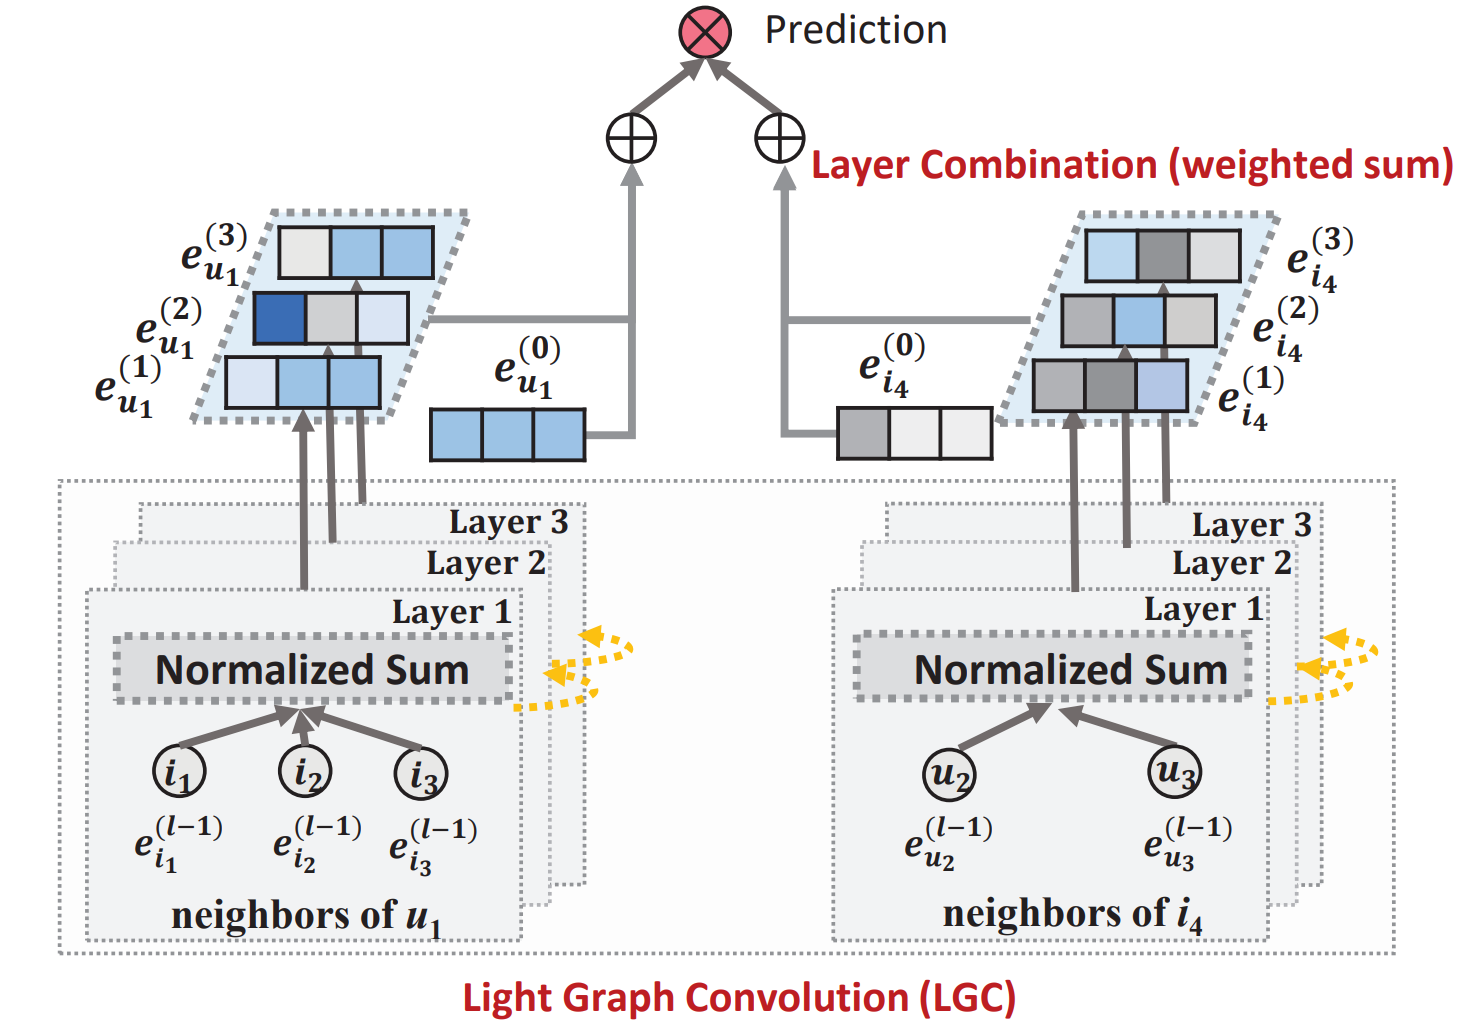
\includegraphics[scale=0.35]{images/Chapter3/lightgcn.png}
    \caption{Thiết kế của LightGCN.}
\end{figure}

\subsubsection{Biểu diễn ma trận của các phép toán}
\noindent Để tiện tính toán trên máy, các tác giả của LightGCN lập ra các phép toán tích chập dưới dạng ma trận. Đầu tiên, ta có ma trận tương tác $\mathbf{R} \in \mathbb{R}^{|U|\times|I|}$, như công thức \eqref{adj-mat-from-R}, ta có ma trận kề:
\begin{equation}
    \mathbf{A} = \begin{pmatrix}
        \mathbf{0} & \mathbf{R} \\
        \mathbf{R}^T & \mathbf{0}
    \end{pmatrix},
\end{equation}
Với các giá trị ban đầu của embedding (lớp 0), ta lập ma trận $\mathbf{E}^{(0)} \in \mathbb{R}^{(|U| + |I|) \times d}$ với $d$ là số chiều embedding, dòng thứ $i$ của $\mathbf{E}^{(0)}$ là $\mathbf{e}_i^{(0)}$. Ta có dạng ma trận của công thức \eqref{lightgcn-neiagg} là:
\begin{equation}
    \mathbf{E}^{(l+1)} = (\mathbf{D}^{-\frac{1}{2}} \mathbf{A} \mathbf{D}^{-\frac{1}{2}}) \mathbf{E}^{(l)},
\end{equation}
trong đó, $\mathbf{D}$ là ma trận đường chéo, cho biết bậc của node trong đồ thị tương tác với kích thước $(|U| + |I|) \times (|U| + |I|)$, có nghĩa là giá trị $D_{ii}$ trong ma trận cho biết số lượng node láng giềng của $i$ trong đồ thị. Như vậy, embedding tổng hợp cuối cùng được định nghĩa là:
\begin{equation}
    \begin{aligned}
        \mathbf{E} & = \alpha_0 \mathbf{E}^{(0)} + \alpha_1 \mathbf{E}^{(1)} + \alpha_2 \mathbf{E}^{(2)} + ... + \alpha_L \mathbf{E}^{(L)} \\
                   & = \alpha_0 \mathbf{E}^{(0)} + \alpha_1 \tilde{\mathbf{A}} \mathbf{E}^{(0)} + \alpha_2 \tilde{\mathbf{A}}^2 \mathbf{E}^{(0)} + ... + \alpha_L \tilde{\mathbf{A}}^L \mathbf{E}^{(0)}
    \end{aligned}
    \label{eq:lightgcn-encoder}
\end{equation}
trong đó, $\tilde{\mathbf{A}} = \mathbf{D}^{-\frac{1}{2}} \mathbf{A} \mathbf{D}^{-\frac{1}{2}}$.


\section{Áp dụng mô hình Học Tự Giám Sát trên đồ thị tương tác người dùng -- sản phẩm}
\noindent Đã nhắc đến ở phần \ref{2.2.2-reprensentation-learning} và \ref{3.2-graph-learning-recommender}, việc học biểu diễn đã bước một bước tiến mới trong việc khai thác kết nối bậc cao hơn trong đồ thị người dùng -- sản phẩm. Tuy nhiên, ngoài những bất cập nói chung của hệ thống gợi ý nói chung (phần \ref{2.1.3-rec-issues}), việc kết hợp học trên đồ thị với gợi ý hiệu quả nhưng vẫn còn đang gặp một vài hạn chế \cite{SGL}.

\begin{itemize}
    \item[(1)] Tín hiệu học giám sát thưa thớt: vấn đề này cũng đã được đề cập. Phần lớn các model có thiết kế dạng học giám sát, tuy nhiên theo ta biết đối với tương tác người dùng với sản phẩm thì dữ liệu quan sát được là rất thưa so với toàn bộ không gian tương tác. Điều này khiến cho việc học biểu diễn không đạt hiệu quả như mong đợi.
    
    \item[(2)] Ảnh hưởng bởi nhiễu: vì hầu hết dữ liệu phản hồi của người dùng đối với sản phẩm lại là phản hồi ngầm thay vì là tường minh \cite{denoise-implicit-feedback} nên các tương tác quan sát được thường xuyên có chứa nhiễu bởi rất nhiều lý do, ví dụ người dùng bị lừa mua sản phẩm... Cơ chế tích chập của mạng tích chập đồ thị làm phóng đại ảnh hưởng của các tương tác lên việc học biểu diễn nên quá trình huấn luyện dễ bị ảnh hưởng do nhiễu trong tương tác.
    
    \item[(3)] Phân phối dữ liệu bị lệch: các tương tác quan sát được thường có phân phối lũy thừa \cite{power-law-dist}. Các sản phẩm bậc thấp thì thiếu tín hiệu giám sát, trong khi đó các sản phẩm có bậc cao thì lại xuất hiện thường xuyên hơn trong tác vụ Neighborhood aggregation và Supervised loss nên có ảnh hưởng nhiều hơn đến học biểu diễn.
\end{itemize}

Học tự giám sát mở ra một con đường mới cho việc giải quyết vấn đề dữ liệu thưa của bài toán hệ thống gợi ý. Mặc dù không có một định nghĩa rõ ràng nào về  việc áp dụng học tự giám sát lên hệ thống gợi ý (SSR), tuy nhiên ta có thể tóm tắt sơ qua về một số đặc điểm \cite{survey:ssl-for-rec-sys} cần lưu ý của SSR như sau:

\begin{itemize}
    \item[] \textbf{Thứ nhất}, mô hình thu được nhiều tín hiệu giám sát hơn bằng việc bán tự động khai thác chính dữ liệu thô ban đầu. Đây là ý tưởng cốt lõi của bất kỳ bài toán học tự giám sát nào từ trước đến nay.
    
    \item[] \textbf{Thứ hai}, ta sử dụng pretext task để train/pre-train mô hình gợi ý với dữ liệu tăng cường. Đây chính là điều khiến SSR khác với các phương pháp tiếp cận khác dùng để giải quyết bài toán hệ thống gợi ý hiện nay.
    
    \item[] \textbf{Thứ ba}, nhiệm vụ gợi ý đóng vai trò là nhiệm vụ chính, pretext task là nhiệm vụ phụ với vai trò tăng cường hiệu quả của nhiệm vụ gợi ý.
\end{itemize}

Hiện nay có rất nhiều phương thức tiếp cận SSR. Nhìn chung, mỗi model SSR chứa hai thành phần \cite{survey:ssl-for-rec-sys} chính: Encoder $\bm{f_\theta}$ và Projection head $\bm{g_\varphi}$. Encoder có thể là một mạng neuron (GNN, Multi-layer Perception...) với tập tham số học $\Theta$ và có nhiệm vụ học cách biểu diễn (embedding) $\mathbf{E}$ cho người dùng và sản phẩm từ dữ liệu. Projection head có cấu trúc đơn giản, có thể là một hàm tuyến tính, mapping, hoặc một mạng neuron đơn giản và có nhiệm vụ tối ưu hóa các biểu diễn đó cho nhiệm vụ gợi ý và/hoặc cho một nhiệm vụ pretext nào đó. Trong phạm vi khóa luận này, thành phần Projection head sẽ được chọn là một hàm đồng nhất. Mạng SSR tập trung giải bài toán sau:
\begin{equation}
    f_\theta, g_\varphi, \mathbf{E} = \underset{f_\theta, g_\varphi}{arg min}\mathcal{L}\left(g_\varphi(f_\theta(\mathcal{D}, \tilde{\mathcal{D}}))\right),
\end{equation}
với $\mathcal{D}$ và $\tilde{\mathcal{D}}$ dữ liệu ban đầu và đã tăng cường, $\mathcal{L}$ là hàm mất mát kết hợp giữa tác vụ gợi ý $\mathcal{L}_\textit{rec}$ (còn được ký hiệu là $\mathcal{L}_\textit{main}$) và tác vụ học không giám sát $\mathcal{L}_\textit{ssl}$. Từ tổng quát hóa trên, ta có thể phân thành 4 phương thức \cite{survey:ssl-for-rec-sys} SSR chủ yếu: \textbf{Contrastive Learning}, \textbf{Generative}, \textbf{Predictive} và \textbf{Hyrbrid}.
\begin{itemize}
    \item[] \textbf{Contrastive}: Kéo những bản sao tăng cường, gọi là các view, của cùng một instance (người dùng/sản phẩm) lại gần nhau, đẩy những view khác instance ra xa nhau trong không gian nhúng.\\
    \begin{minipage}{\linewidth}
        \vspace*{+5mm}
        \centering
        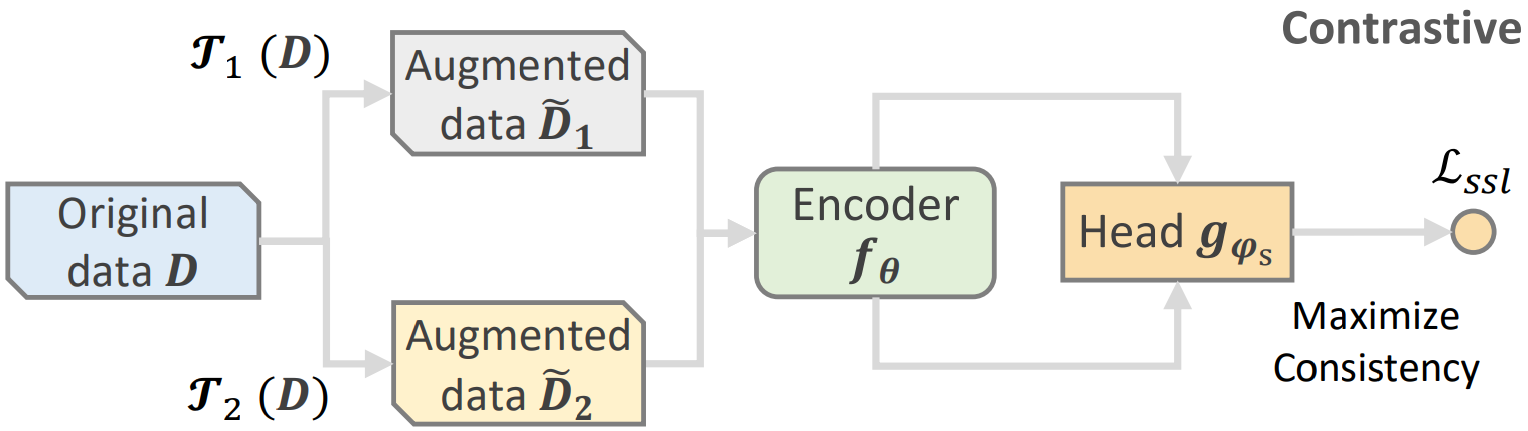
\includegraphics[scale=0.3]{images/Chapter3/contras_ssr.png}
        \captionof{figure}[Sơ đồ tổng thể phương pháp Contrastive trong bài toán Self-supervised Recommendation.]{Sơ đồ tổng thể phương pháp Contrastive trong bài toán Self-supervised Recommendation. Thành phần Head $\bm{g_{\varphi_s}}$ ở đây có nhiệm vụ giúp model phân biệt tốt hơn những mẫu dữ liệu nào là giống nhau, những mẫu dữ liệu nào là khác nhau.}
    \end{minipage}
    
    \item[] \textbf{Generative}: Dự đoán một phần của data gốc ban đầu đã bị làm hỏng.\\
    \begin{minipage}{\linewidth}
        \vspace*{+5mm}
        \centering
        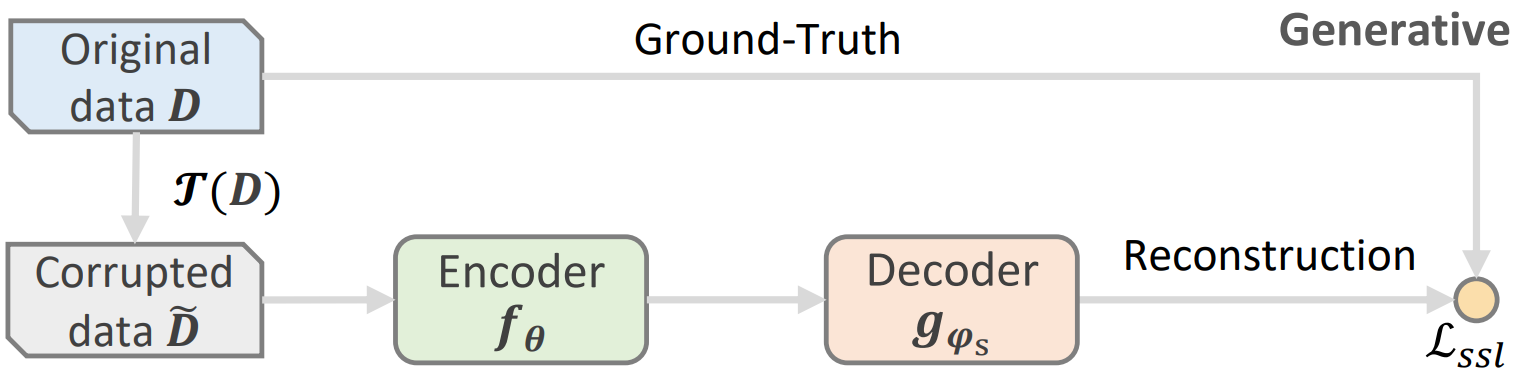
\includegraphics[scale=0.3]{images/Chapter3/gen_ssr.png}
        \captionof{figure}[Sơ đồ tổng thể phương pháp Generative trong bài toán Self-supervised Recommendation.]{Sơ đồ tổng thể phương pháp Generative trong bài toán Self-supervised Recommendation. Thành phần Decoder $\bm{g_{\varphi_s}}$ ở đây là một loại Head đặc biệt mà có nhiệm vụ tái tạo lại dữ liệu gốc từ dữ liệu embedding của dữ liệu đã bị làm hỏng. Sau đó dữ liệu này và dữ liệu gốc thực sự sẽ được so sánh với nhau.}
    \end{minipage}
    
    \item[] \textbf{Predictive}: Khá giống với phương pháp Generative. Nhưng trong khi mục tiêu của generative method là dự đoán data gốc, phương pháp Predictive, những mẫu dữ liệu mới hoặc nhãn dữ liệu mới sẽ được sinh ra để giúp tác vụ pretext.\\
    \begin{minipage}{\linewidth}
        \vspace*{+5mm}
        \centering
        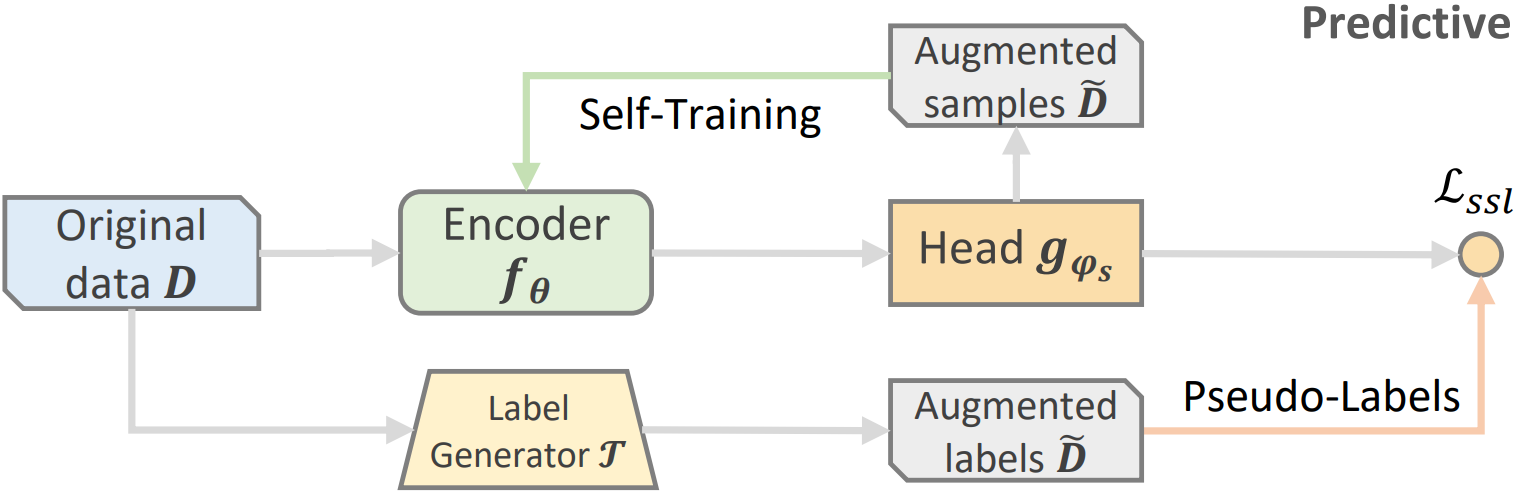
\includegraphics[scale=0.3]{images/Chapter3/pred_ssr.png}
        \captionof{figure}[Sơ đồ tổng thể phương pháp Predictive trong bài toán Self-supervised Recommendation.]{Sơ đồ tổng thể phương pháp Predictive trong bài toán Self-supervised Recommendation. Có thể chia phương pháp ra hai loại: dựa trên mẫu dữ liệu (sample-based) và dựa trên nhãn giả (pseudo-label-based). Loại thứ nhất tập trung dự đoán những mẫu dữ liệu nào là có thông tin hữu ích nhất cho pretext; loại thứ hai sinh ra nhãn giả cho dữ liệu dùng một Label Generator (có thể là một encoder khác) để giúp cho Encoder chính $\bm{f_\theta}$.}
    \end{minipage}
    
    \item[] \textbf{Hybrid}: Mỗi pretext task trên đều có ưu điểm riêng và đều có thể tận dụng được các self-supervision signal khác nhau. Hybrid method (phương pháp lai) tích hợp các pretext task khác nhau vào cùng một SSR model.\\
    \begin{minipage}{\linewidth}
        \vspace*{+5mm}
        \centering
        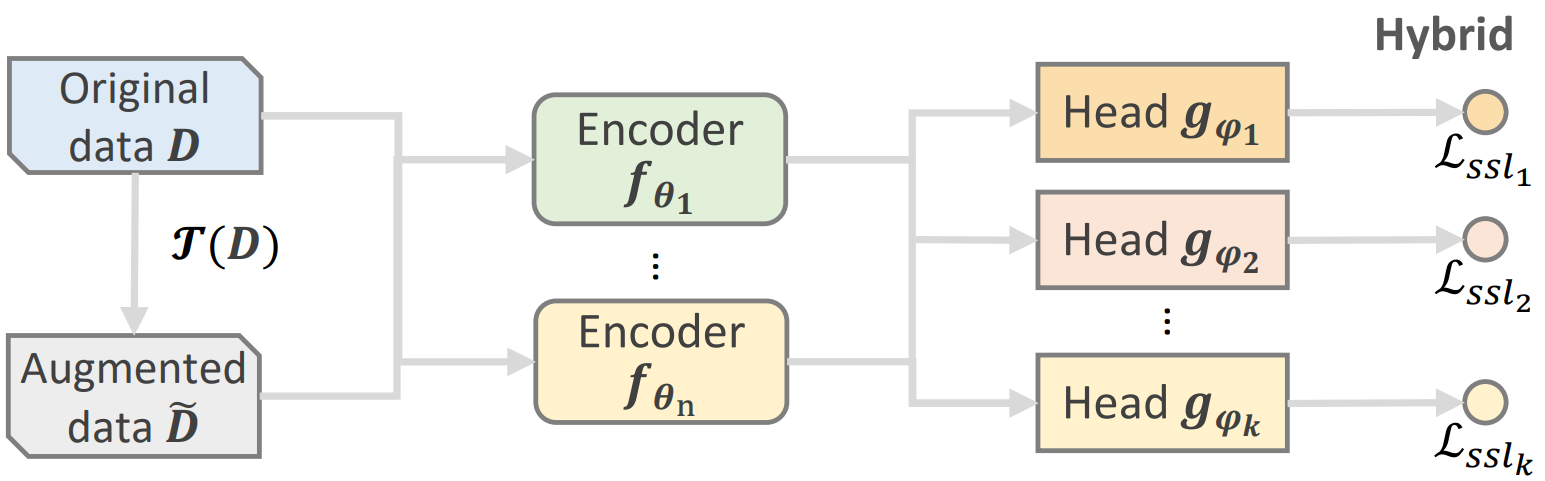
\includegraphics[scale=0.3]{images/Chapter3/hybrid_ssr.png}
        \captionof{figure}{Sơ đồ tổng thể phương pháp Hybrid trong bài toán Self-supervised Recommendation.}
    \end{minipage}
\end{itemize}

Trong phạm vi khóa luận này, ta sẽ tập trung giải thích việc áp dụng \textbf{Contrastive Learning} vào SSR và phân tích hiệu quả mà nó mang lại. Cụ thể hơn về việc áp dụng Contrastive Learning trong bài toán SSR như thế nào, ta mô tả chi tiết ở phần sau. Ngoài Contrastive learning, những phương pháp khác vẫn có rất nhiều tiềm năng phát triển và đáng được nghiên cứu trong tương lai, vậy nên ta chỉ mô tả ý tưởng chính chứ không tiếp tục đào sâu ở các phần sau.

\subsection{Kiến trúc tổng quát} \label{3.3.1-general-architecture}
% \subsubsection{Encoder}
% \subsubsection{Project head}
% Để cải thiện hệ thống gợi ý, kiến trúc của hệ thống sẽ bao gồm hai phần như trên hình. Phần thứ nhất, tác vụ gợi ý trên mạng học sâu đồ thị, đóng vai trò chính. Phần thứ hai, áp dụng contrastive learning với dữ liệu được tăng cường (dữ liệu này được tạo ra từ chính đồ thị gốc ban đầu, điều này sẽ giúp cải thiện việc học biểu diễn, từ đó bổ trợ, tối ưu cho cho tác vụ gợi ý.

\noindent Về mặt phương pháp áp dụng học tự giám sát, ta có hai thành phần chính. Phần thứ nhất đóng vai trò chính, học các biểu diễn cho node trong đồ thị và đưa ra dự đoán cho tác vụ gợi ý. Phần thứ hai áp dụng Học tương phản (Contrastive learning) với dữ liệu được tăng cường để cải thiện học biểu diễn, từ đó tối ưu cho tác vụ gợi ý.

\begin{figure}[H]
    \centering
    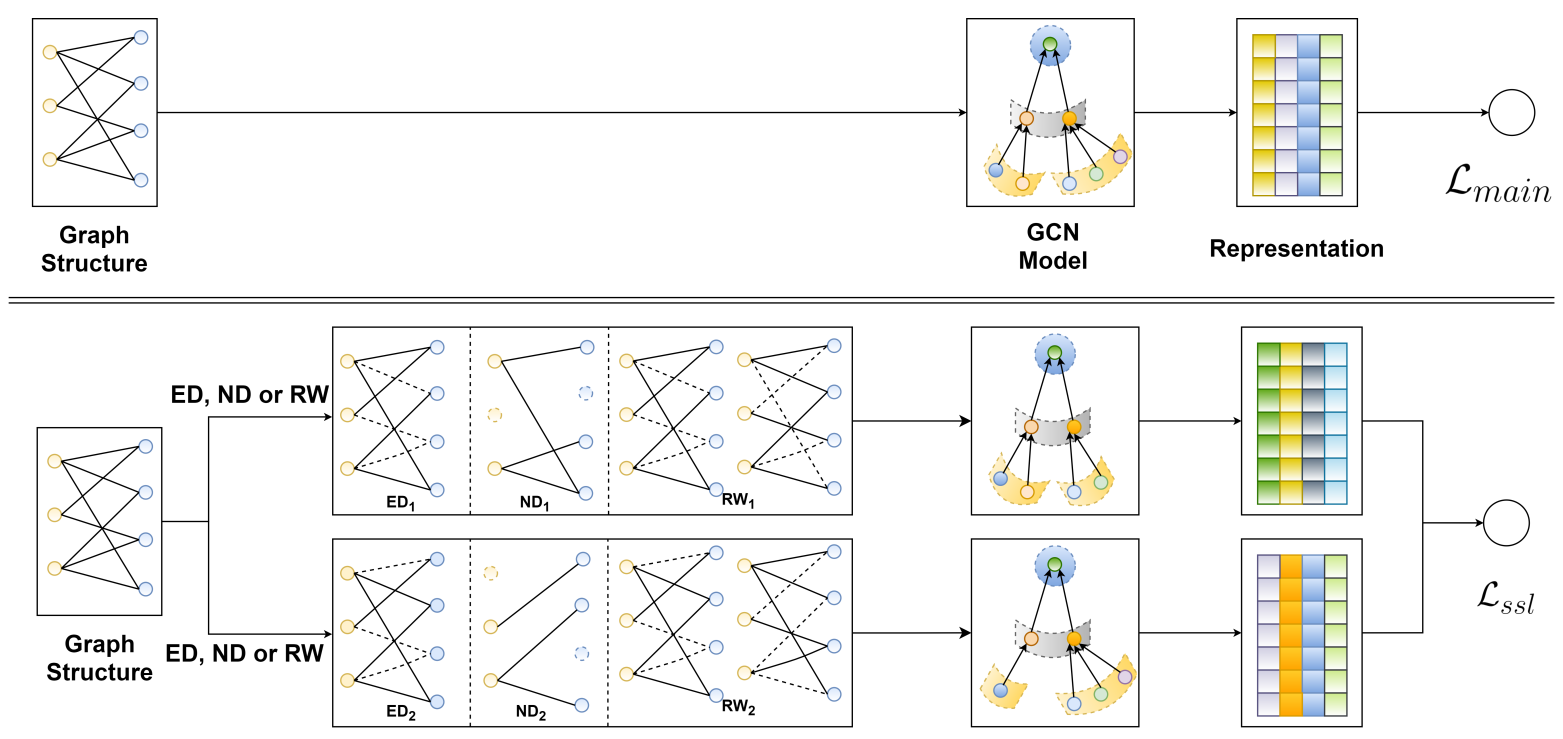
\includegraphics[scale=0.35]{images/Chapter3/sgl.png}
    \caption[Tác vụ chính và phụ của Contrastive learning.]{Trên: tác vụ chính (main task) cho gợi ý. Dưới: tác vụ phụ (pretext task) tối ưu học biểu diễn (Hình ảnh được trích từ bài báo của Wu \cite{SGL}).}
\end{figure}

Đối với việc tăng cường dữ liệu, hiện tại có rất nhiều cách tiếp cận, vì ma trận kề của đồ thị tương tác chính là ma trận đặc trưng của nó nên chỉ cần tập trung vào tăng cường cấu trúc đồ thị là đủ. Nói về đại ý, ta cần tạo các tăng cường dựa trên cấu trúc đồ thị gốc, làm thay đổi ma trận kề của đồ thị. Ta định nghĩa hai tăng cường của cùng một node sẽ được coi như là một positive pair và của các node khác nhau được coi như là negative pair. Nhiệm vụ tự giám sát phụ trợ sẽ thúc đẩy tính nhất quán giữa các positive pair, trong khi đó ép ra xa nhau đối với các negative pair trong không gian nhúng. Nhờ đó, ta có thể suy ra embedding một cách tốt hơn, từ việc quan sát và rút trích những đặc điểm, những cấu trúc bên dưới hoặc những khuôn mẫu đặc trưng nào đó của dữ liệu. 
% https://arxiv.org/pdf/2301.12189v1.pdf
% https://arxiv.org/pdf/2212.11491.pdf

\subsection{Áp dụng tăng cường dữ liệu}
\noindent Trong phạm vi khóa luận này, ta sẽ áp dụng các phương thức tăng cường \textbf{Edge dropout}, \textbf{Node dropout} và \textbf{Random walk} nhằm tạo ra các view khác nhau của node.

Về chi tiết mô tả tăng cường, ta đã đề cập ở phần \ref{3.1-data-aug}. Khi huấn luyện, ở mỗi epoch, ta sẽ tạo ra hai view cho mỗi node. Với hai phương pháp Edge Dropout và Node Dropout ta sẽ chọn lược bỏ một số cạnh/node với xác suất $\rho$. Hai view của các node trong Edge/Node dropout được chia sẻ và sử dụng chung trên các lớp trong mạng học sâu đồ thị. Riêng với Random Walk, ta sẽ chọn giữ toàn bộ node, với mỗi node, ta bước qua một vài node lân cận một cách ngẫu nhiên, với xác suất bỏ cạnh đi qua là $\rho$. Thêm nữa, để tăng tính ngẫu nhiên, tại mỗi lớp trong mạng học sâu đồ thị, ta sẽ tạo ra hai view khác nhau cho tăng cường Random walk.

Với ký hiệu như đã định nghĩa ở phần \ref{3.2.3-GNN-on-rec}, ta gọi embedding của hai view của cùng một node $v$ là $\mathbf{e}_v'$ và $\mathbf{e}_v''$.

\subsection{Học Tương Phản trên dữ liệu tăng cường}
\noindent Về mặt thống kê, các mô hình học máy được chia thành loại genrative và discriminative \cite{ssl-genorcont}. Hầu hết các nhiệm vụ học biểu diễn đều hy vọng sẽ mô hình hóa được các mối quan hệ giữa điểm dữ liệu đầu vào (input), vậy nên trong một thời gian dài, mọi người tin rằng mô hình Generative là lựa chọn duy nhất cho việc học biểu diễn.

Ở phần \ref{2.4-ssl}, ta biết rằng khi áp dụng Học tự giám sát, ta có rất nhiều cách tiếp cận khi mô hình học này lên mạng học sâu đồ thị. Ở phần \ref{3.2-graph-learning-recommender} ta cũng nhận ra để có được một biểu diễn của đồ thị đủ tốt và mang lại hiệu quả, các mô hình cần nắm bắt được các thông tin cần thiết từ cả thuộc tính nút và cấu trúc liên kết của đồ thị. Học tương phản nói riêng và mô hình discriminative nói chung đã mở ra một cánh cửa mới cho việc học biểu diễn như DeepInfoMax \cite{DeepInfoMax}, MoCo \cite{MoCo}, SimCLR \cite{SimCLR},... Hơn nữa, tính hiệu quả của nó cũng đã được chứng minh bởi Wu và các đồng nghiệp \cite{SGL}. Học tương phản sẽ được áp dụng như là một phương thức hay nói cách khác nó đóng vai trò không thể thiếu khi ta muốn áp dụng mô hình học tự giám sát trên mạng học sâu đồ thị nhằm làm tăng hiệu quả cho tác vụ gợi ý. Để áp dụng được phương pháp này, ta cũng cần một hàm mất mát phù hợp. Một loại hàm mất mát được áp dụng phổ biến và rất hiệu quả đối với học tự giám sát nói chung là InfoNCE \cite{InfoNCE, ssl-genorcont}, có dạng tổng quát như sau:
\begin{equation}
    \mathcal{L}_\textit{ssl} = \mathbb{E}_{z, z^+, z^-}\left[-\log{\frac{\exp(z^T z^+)}{\exp(z^T z^+) + \exp(z^T z^-)}}\right],
    \label{eq:general-NCE}
\end{equation}
với $\mathbb{E}[\cdot]$ là kì vọng, $\exp(\cdot)$ là hàm mũ cơ số $e$, $z$ là biểu diễn của một mẫu dữ liệu (tạm gọi là $x$), $z^+$ là biểu diễn của một mẫu dữ liệu mà giống với $x$, và $z^-$ là biểu diễn của một mẫu dữ liệu mà không giống với $x$. Khi cực tiểu hóa $\mathcal{L}_\textit{ssl}$, ta sẽ thúc đẩy tính nhất quán giữa $z$ và $z^+$, ép sự phân kì giữa $z$ và $z^-$. Nếu tập dữ liệu chứa nhiều mẫu dữ liệu không giống với $x$ thì công thức trên có dạng:
\begin{equation}
    \mathcal{L}_\textit{ssl} = \mathbb{E}_{z, z^+, z^k}\left[-\log{\frac{\exp(z^T z^+)}{\exp(z^T z^+) + \sum_{x^k \nsim x}{\exp(z^T z^k)}}}\right],
    \label{eq:more-dissim-NCE}
\end{equation}
với $x^k$ là những mẫu dữ liệu không giống với $x$. Để thực sự áp dụng công thức này vào học gợi ý, ta cần phải biến đổi đôi chỗ.

\subsubsection{Hàm mất mát InfoNCE}
\noindent Ở công thức \eqref{eq:general-NCE} và \eqref{eq:more-dissim-NCE}, ta nhắc đến mẫu dữ liệu với tính chất ``giống'' và ``không giống'' nhau, tức là trong tập dữ liệu, nếu xét về tính chất, đặc trưng,... thì hai mẫu dữ liệu đó có tập thuộc tính tương tự nhau, và ngược lại nếu như hai mẫu dữ liệu đó không giống nhau. Đối với bài toán gợi ý trên đồ thị thì như ta đã định nghĩa ở phần \ref{3.3.1-general-architecture}, cặp node positive pair sẽ được coi như là giống nhau, cặp negative pair được coi như là khác nhau. Với học gợi ý, Wu \cite{SGL} đề xuất một hàm mất mát phục vụ cho việc Học tương phản như sau trên ý tưởng của InfoNCE:
\begin{equation}
    \mathcal{L}_\textit{ssl}^\textit{user} = \sum_{u \in U}{-\log{\frac{\exp(s(\mathbf{e}_u', \mathbf{e}_u'') / \tau)}{\sum_{v \in U}{\exp(s(\mathbf{e}_u', \mathbf{e}_v'') / \tau)}}}},
\end{equation}
trong đó, $\tau$ là 1 hyper-parameter gọi là temperature trong softmax, $s(\cdot)$ đo sự tương đồng giữa 2 vector, dùng độ tương đồng cosine, công thức \eqref{eq:cosine-sim}. Ta có thể áp dụng công thức hàm mất mát trên tương tự cho sản phẩm. Từ đó, ta có hàm mất mát cho quá trình Học tương phản như sau:
\begin{equation}
    \mathcal{L}_\textit{ssl} = \mathcal{L}_\textit{ssl}^\textit{user} + \mathcal{L}_\textit{ssl}^\textit{item}.
\end{equation}

Wu và các đồng nghiệp \cite{SGL} phân tích hàm mất mát trên và đưa ra ưu điểm là nó giúp mô hình phân biệt các biểu diễn của những node khác nhau tốt hơn thông qua \textit{Hard negative mining}. Cụ thể là với những cặp negative pair mà có biểu diễn giống nhau, khó phân biệt, hàm mất mát sẽ có nhiều ảnh hưởng hơn so với những cặp negative pair dễ phân biệt được với nhau. Thông qua sự điều chỉnh phù hợp của tham số $\tau$, ta cũng sẽ điều chỉnh được độ nhạy của Hard negative mining.

Hàm mất mát trên có tính hiệu quả cao, tuy nhiên cũng không phải là không có bất cập. Ngoài InfoNCE ra, ta cũng sẽ thử nghiệm thêm với hai loại hàm mất mát khác nữa là \textbf{Decoupled} \cite{decoupled-loss} và \textbf{Debiased} \cite{debiased-loss}.

\subsubsection{Hàm mất mát Decoupled}

\noindent Theo Yeh và đồng nghiệp \cite{decoupled-loss} tìm hiểu được, hàm mất mát InfoNCE có chứa một hệ số negative-positive-coupling (NPC) giảm hiệu năng tự giám sát của model, đặc biệt là khi batch size nhỏ. Ngoài ra là trong InfoNCE, mô hình rất nhạy cảm với các hyperparameter, tức là các hyperparameter không tối ưu sẽ ảnh hưởng rất nhiều lên việc học tự giám sát một cách tiêu cực. Các tác giả của hàm mất mát Decoupled cho rằng với hàm mất mát của họ, mô hình sẽ tăng hiệu quả huấn luyện hơn mà không cần phải sử dụng batch size lớn. Không những vậy, khi batch size càng lớn thì mô hình càng học tốt hơn. Tổng quát của hàm mất mát này rất đơn giản: từ gốc là hàm mất mát InfoNCE, ta chỉ cần trừ hàm mũ $\exp(s(\mathbf{e}_u', \mathbf{e}_u'') / \tau)$ ra khỏi mẫu. Cụ thể, với các biểu diễn cho gợi ý, công thức hàm mất mát có dạng như sau:
\begin{equation}
    \begin{aligned}
        \mathcal{L}_\textit{decoupled ssl}^\textit{user} & = \sum_{u \in U}{-\log{\frac{\exp(s(\mathbf{e}_u', \mathbf{e}_u'') / \tau)}{\sum_{v \neq u}{\exp(s(\mathbf{e}_u', \mathbf{e}_v'') / \tau)}}}} \\
        & = \sum_{u \in U}{\left[-s(\mathbf{e}_u', \mathbf{e}_u'') / \tau + \log{\left(\sum_{v \neq u}{\exp(s(\mathbf{e}_u', \mathbf{e}_v'') / \tau)}\right)}\right]}.
    \end{aligned}
\end{equation}

\subsubsection{Hàm mất mát Debiased}

\noindent Chuang và đồng nghiệp \cite{debiased-loss} chỉ ra rằng, trong đa phần các model sử dụng Contrastive learning, với mỗi mẫu dữ liệu $x$, chỉ chọn ra một mẫu dữ liệu $x^+$ khác để kết hợp làm positive pair, ví dụ điển hình là mẫu dữ liệu này được trích ra từ bản sao tăng cường; nhưng song song với đó lại chọn nhiều mẫu dữ liệu $x^-$ khác để kết hợp làm negative pair. Bất cập của tiếp cận này là vẫn có khả năng là có một mẫu dữ liệu $x^-$ nào đó mà thực sự giống với $x$ nhưng lại bị thúc đẩy sự phân kì xét về mặt biểu diễn, ví dụ trường hợp hai người dùng khác nhau nhưng có chung tập sản phẩm đã tương tác. Hiện tượng này được Chuang và đồng nghiệp gọi là \textit{thành kiến trong việc lấy mẫu} -- \textit{sampling bias} mà có thể dẫn đến giảm hiệu năng trong thực tế.

Một hàm mất mát lí tưởng mà không có sampling bias trên thực tế không thể đạt được. Vì vậy, Chuang và đồng nghiệp xây dựng một tiếp cận mới để làm giảm tác động tiêu cực của nó -- Debiased. Ý tưởng chính là với tổng hàm mũ $\sum_{v \neq u}{\exp(s(\mathbf{e}_u', \mathbf{e}_v'') / \tau)}$ ở dưới mẫu, ta trừ đi một tỉ lệ của giá trị $\exp(s(\mathbf{e}_u', \mathbf{e}_u'') / \tau)$ để giảm đi tác động của việc phải phân kì các cặp $\mathbf{e}_u'$ và $\mathbf{e}_v''$ mà hai node $u$ và $v$ có thể giống nhau. Cụ thể, ta có phương trình tổng quát sau:
\begin{equation}
    \mathcal{L}_\textit{debiased ssl}^\textit{user} = \sum_{u \in U}{-\log{\frac{\exp(s(\mathbf{e}_u', \mathbf{e}_u'') / \tau)}{\exp(s(\mathbf{e}_u', \mathbf{e}_u'') / \tau) + \textit{Ng}}}},
\end{equation}
trong đó, $\textit{Ng}$ là hàm lấy giá trị lớn nhất $\max(\textit{Ng}', N \cdot \exp(-\frac{1}{t}))$ với $\textit{Ng}'$ là:
\begin{equation}
    \textit{Ng}' = \frac{-N \cdot \tau^+ \cdot \exp(s(\mathbf{e}_u', \mathbf{e}_u'') / \tau) + \sum_{v \neq u}{\exp(s(\mathbf{e}_u', \mathbf{e}_v'') / \tau)}}{1 - \tau^+},
\end{equation}
với $N$ là số lượng node $v \neq u$; $\tau^+$ là xác suất chọn một node $v \neq u$ nào đó mà thực sự giống với $u$, dùng để ước lượng mức độ ảnh hưởng của các cặp negative pair $(\mathbf{e}_u', \mathbf{e}_v'')$ thông qua cặp positive pair $(\mathbf{e}_u', \mathbf{e}_u'')$ khi giảm sampling bias trong tổng $\sum_{v \neq u}{\exp(\cdot)}$. Giá trị mẫu $1 - \tau^+$ dùng để bình thường hóa lại độ lớn của $\textit{Ng}'$ trong trường hợp giá trị trên tử quá nhỏ (gần bằng 0), tức là $\tau^+$ gần bằng 1. Việc tính $\tau^+$ cho mỗi node trong đồ thị là không thực tế, đặc biệt với lượng dữ liệu lớn, nên ta giả định $\tau^+$ đồng nhất với mọi node, và giá trị của nó là xác suất chọn một cặp negative pair bất kì trong toàn bộ tập dữ liệu mà lại thực sự giống nhau. Như vậy, tham số này có thể được ước tính từ tập dữ liệu hoặc là tự điều chỉnh (hyperparameter). Lấy $\max$ với $N \cdot \exp(-\frac{1}{t})$ chẳng qua là để tránh trường hợp lấy $\log$ của số âm; $t$ là hyperparameter khác.


\subsection{Phương án huấn luyện}
\noindent Trong thực tế, tác vụ gợi ý và pretext task (trong khóa luận này là Học tương phản) được kết hợp theo nhiều phương án (scheme) khác nhau tùy thuộc vào tình huống cụ thể. Ở trong phạm vi khóa luận này, ta sẽ sử dụng phương án \textbf{Joint Learning} \cite{survey:ssl-for-rec-sys} để giải quyết bài toán. 

\textbf{Joint Learning}: hiện nay, đa số các cách tiếp cận với học tự giám sát trên hệ thống gợi ý đều áp dụng scheme dạng này, đặc biệt là các phương thức contrastive. Lúc này, pretext task được bổ sung và cùng lúc được tối ưu với tác vụ chính là tác vụ gợi ý qua một encoder chung (ví dụ, trong khóa luận ta đang sử dụng một loại mạng học sâu đồ thị LightGCN). Kết quả tốt nhất ta có thể đạt được bằng cách điều chỉnh hyperparameter $\alpha$. Đây có thể được xem là một dạng multi-task learning.

\begin{figure}[H]
    \centering
    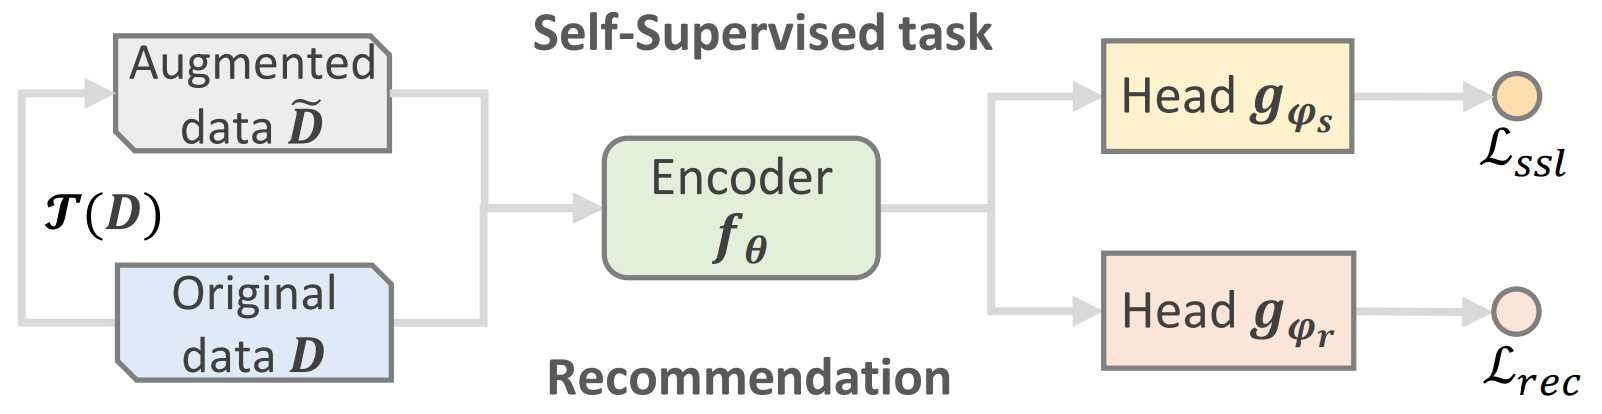
\includegraphics[scale=0.32]{images/Chapter3/jl_scheme.png}
    \caption{Sơ đồ Joint Learning.}
\end{figure}

\noindent Tổng quát hóa, ta giải bài toán tối ưu sau:
\begin{equation}
    f_\theta, g_\varphi, \mathbf{E} = \underset{f_\theta, g_\varphi}{arg min}\left[\mathcal{L}_\textit{rec}(g_{\varphi_r}(f_\theta(\mathcal{D}))) + \alpha \mathcal{L}_\textit{ssl}(g_{\varphi_s}(f_\theta(\tilde{\mathcal{D}})))\right],
\end{equation}
trong đó, hyperparameter $\alpha$ giúp điều chỉnh mức độ của tín hiệu học tự giám sát. Với công thức trên, ta sẽ sử dụng một hàm mất mát cho multi-task training đơn giản bằng cách kết hợp hai hàm mất mát của tác vụ gợi ý và tác vụ tự giám sát nhằm tối ưu cho hệ thống. Ta đi tìm cực tiểu cho hàm sau:
\begin{equation}
    \mathcal{L} = \mathcal{L}_\textit{rec} + \lambda_1 \mathcal{L}_\textit{ssl} + \lambda_2 \lVert \Theta \rVert_2^2,
\end{equation}
với $\Theta$ là tập hợp các tham số học của model; $\lambda_1$ và $\lambda_2$ lần lượt là các hyperparameter để kiểm soát mức độ ảnh hưởng của SSL và $L_2$ regularization, tương ứng. Với các kiến thức đã nói trước, ta có hàm mất mát sau cho mô hình học không giám sát trên đồ thị cho hệ thống gợi ý:
\begin{equation}
    \mathcal{L} = \mathcal{L}_\text{BPR} + \lambda_1 \mathcal{L}_\textit{ssl} + \lambda_2 \lVert \mathbf{E}^{(0)} \rVert_2^2,
\end{equation}
với $\mathcal{L}_\text{BPR}$ là hàm mất mát BPR \footnote{Trong hàm mất mát BPR cũng có regularization của tham số học của model. Ta sẽ kết hợp nó với regularization của Joint learning, và hàm mất mát BPR cũng sẽ được đơn giản hóa trở thành một hàm tổng $\ln(\cdot)$ duy nhất.}, $\mathcal{L}_\textit{ssl}$ là một trong ba hàm mất mát sử dụng việc học tương phản đã được định nghĩa ở phần trước, $\mathbf{E}^{(0)}$ là embedding của node (và cũng là tham số học) tại lớp thứ 0 của LightGCN. Tương tự như vậy, ta có Encoder $f_\theta$ là kiến trúc của LightGCN (công thức \ref{eq:lightgcn-encoder}).


% maximize mutual information như nào
% \begin{equation}
% L = E_{x,x^+,x^-} [-\log \frac{e^{f(x)} \cdot f(x^+)}{e^{f(x)} \cdot f(x^+) + e^{f(x)} \cdot f(x^-)}]
% \end{equation}

Ngoài Joint Learning (JL Scheme) ra, một số scheme khác có thể được áp dụng, tuy nhiên sẽ không được áp dụng trong phạm vi khóa luận này đó là \textbf{Pretraining and fine-tuning} (PF Scheme) và \textbf{Integrated Learning} (IL Scheme) \cite{survey:ssl-for-rec-sys}. Ta sẽ giới thiệu đôi nét về việc áp dụng hai phương án huấn luyện này và để dành việc khảo sát độ hiệu quả của hai phương án này cho các nghiên cứu trong tương lai.

\textbf{Pretraining and fine-tuning}: Phương án này cũng được sử dụng khá phổ biến. Đầu tiên, với pretext task, ta sẽ pretrain trên dữ liệu được tăng cường. Sau đó, ta sẽ sử dụng pretrain encoder thu được ở trên để fine-tune cho dữ liệu gốc. Cách này thường được dùng để huấn luyện các model SSR có dạng BERT, trong đó giai đoạn pretrain sẽ được áp dụng trên masked-based augmentation của input và sẽ được fine-tune trên dữ liệu chính. Ngoài ra còn được dùng khi pretext task để pre-train là contrastive method.
\begin{figure}[H]
    \centering
    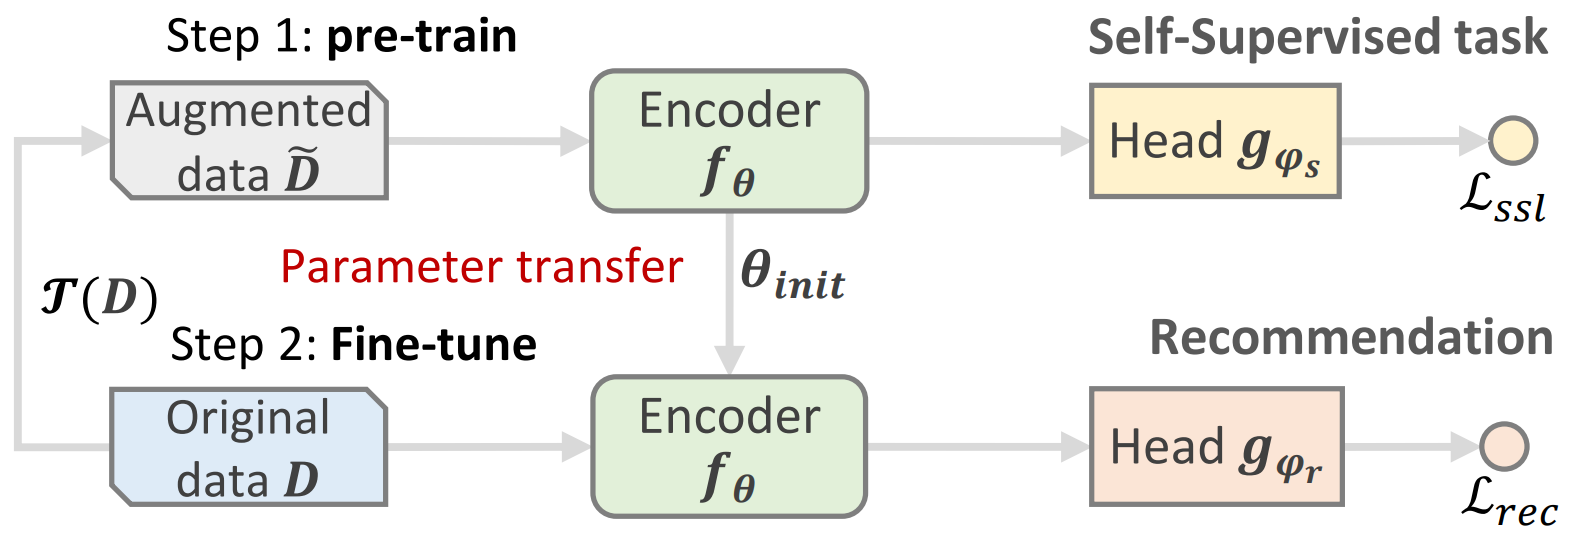
\includegraphics[scale=0.32]{images/Chapter3/pf_scheme.png}
    \caption{Sơ đồ Pretraining and fine-tuning}
\end{figure}

\textbf{Integrated Learning}: Khác với JL Scheme và PF Scheme, IL scheme thường được ít chú ý và biết đến. Lúc này pretext task và recommendation task được căn chỉnh sao cho output của cả hai là tương tự nhau.
\begin{figure}[H]
    \centering
    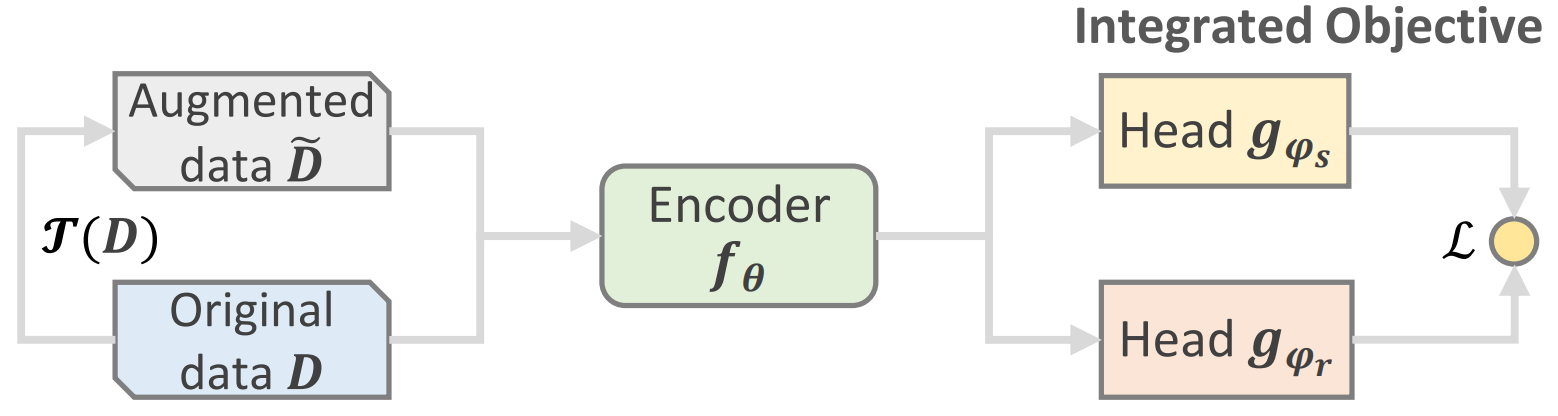
\includegraphics[scale=0.32]{images/Chapter3/il_scheme.png}
    \caption{Sơ đồ Integrated Learning}
\end{figure}

\subsection{Mã giả của thuật toán}
\noindent Sau đây là mô tả thuật toán tối ưu hóa các tham số của một model học tự giám sát trên đồ thị cho hệ thống gợi ý đã được mô tả ở trên. Ta có thuật toán SSL\_REC nhận đầu vào là các tham số $\mathbf{A}$ là ma trận kề của đồ thị tương tác, $\Theta$ là các tham số học ($\mathbf{E}^{(0)}$), cùng với đó là các tham số regularization $\lambda_1$ và $\lambda_2$. SSL\_REC sẽ đi tìm cực tiểu cho $\mathcal{L}$ bằng cách tìm giá trị cho $\mathbf{E}^{(0)}$ thông qua thuật toán Gradient descent với learning rate $\eta$. Ngoài ra ta định nghĩa đầu vào của các hàm sau:
\begin{itemize}
    \item[] \textbf{Encoder} $f_\theta(X, \mathbf{A})$: với $X$ là tham số của model, $\mathbf{A}$ là ma trận kề của đồ thị. Encoder trả về embedding cuối cùng $\mathbf{E}$ của model. Để ý là ta đang dùng kí hiệu $X$ thay vì $\mathbf{E}^{(0)}$ để dụng ý rằng $X$ là \textbf{biến} của hàm, trong khi $\mathbf{E}^{(0)}$ là một \textbf{giá trị} của $X$.

    \item[] \textbf{Hàm mất mát BPR} $\mathcal{L}_\text{BPR}(\mathbf{E})$: với $\mathbf{E}$ là embedding cuối cùng của model.

    \item[] \textbf{Hàm mất mát cho Học tương phản} $\mathcal{L}_\textit{ssl}(\mathbf{E}', \mathbf{E}'')$: với $\mathbf{E}'$ và $\mathbf{E}''$ là các embedding cuối cùng của hai đồ thị tăng cường được tạo ra. Để có được $\mathbf{E}'$ và $\mathbf{E}''$ thì ta chỉ cần lấy kết quả trả về của Encoder thông qua hai ma trận kề của các đồ thị tăng cường.
\end{itemize}
Ngoài ra ta cũng định nghĩa hàm $\mathcal{F}_\text{aug}(\mathbf{A})$ sẽ trả về ma trận kề của hai đồ thị tăng cường khác nhau từ ma trận kề gốc.

\clearpage
\noindent \textbf{Mã giả của thuật toán}
\begin{algorithm}[H]
    % \small
    \fontsize{14}{15}\selectfont
    \caption{SSL\_REC}
    \begin{algorithmic}[1]
        \Procedure{SSL\_REC}{$\mathbf{E}^{(0)}$, $\mathbf{A}$, $\lambda_1$, $\lambda_2$}
            \State initialize $\mathbf{E}^{(0)}$
            \Repeat
                \State $\mathbf{A}', \mathbf{A}'' \gets \mathcal{F}_\text{aug}(\mathbf{A})$
                
                \vspace*{+3mm}
                \State $\mathcal{L}(X) \gets \mathcal{L}_\text{BPR}\left[f_\theta(X, \mathbf{A})\right] + \lambda_1 \mathcal{L}_\textit{ssl}\left[f_\theta(X, \mathbf{A}'), f_\theta(X, \mathbf{A}'')\right] + \lambda_2 \lVert X \lVert_2^2$
                
                \vspace*{+3mm}
                \State $\nabla \mathcal{L}(\mathbf{E}^{(0)}) \gets \dfrac{\partial}{\partial X}\mathcal{L} \; \Bigr|_{\substack{X = \mathbf{E}^{(0)}}}$

                \vspace*{+3mm}
                \State $\mathbf{E}^{(0)} \gets \mathbf{E}^{(0)} - \eta \cdot \nabla \mathcal{L}(\mathbf{E}^{(0)})$
            \Until{convergence}
        \EndProcedure
    \end{algorithmic}
\end{algorithm}

% ssl method có thể đc áp dụng trên model graph bất kỳ
% 4. Phân tích SGL


\chapter{Các kết quả thí nghiệm}
\label{Chapter4}

\noindent Trong chương này, nhóm nghiên cứu sẽ trình bày các thiết lập ban đầu và kết quả thí nghiệm mà nhóm đã cài đặt và thu được dựa trên các bài báo đã nghiên cứu. Bộ dữ liệu được sử dụng sẽ là những bộ dữ liệu thường được sử dụng để kiểm chứng hiệu quả mà các phương pháp áp dụng lên mô hình gợi ý hiện nay thường dùng. Ngoài tái hiện, kiểm chứng kết quả của bài báo gốc, nhóm cũng tiến hành thêm một vài thí nghiệm nhằm thử nghiệm cải tiến mô hình được đề xuất với mục đích nhằm giảm tác động tiêu cực của các hạn chế mà bài báo gốc vẫn chưa giải quyết được. Cùng với đó, nhóm sẽ phân tích, nhận xét các kết quả đạt được và so sánh với các mô hình học đi trước.

\section{Môi trường thí nghiệm và thiết lập thí nghiệm}

\subsection{Dữ liệu thí nghiệm}

\subsubsection{Mô tả}
\noindent Nhóm sẽ tiến hành cài đặt, thử nghiệm độ hiệu quả của mô hình vừa tìm hiểu được. Nhóm đã chọn ra 3 bộ dữ liệu \textbf{Yelp2018}, \textbf{Amazon Book}, \textbf{iFashion}, đây là những bộ dữ liệu có độ phổ biến cao (hay được sử dụng dùng để chứng minh kết quả) của hệ thống gợi ý để đánh giá kết quả thu được.
\begin{itemize}
    \item[] \textbf{Yelp2018}: Bộ dữ liệu được trích ra từ cuộc thi yelp năm 2018, trong đó các doanh nghiệp tại địa phương như nhà hàng, quán bar... được đánh giá và xem như là các ``sản phẩm''.

    \item[] \textbf{Amazon Book}: Được trích từ tập dữ liệu đánh giá Amazon-review. Amazon Book chứa thông tin đánh giá của người dùng với các sản phẩm sách của Amazon từ năm 1996 đến 2014.

    \item[] \textbf{iFashion}: Bộ dữ liệu công khai của nền tảng iFashion của Taobao (Alibaba Group), gồm các sản phẩm thời trang, các trang bán hàng online và đánh giá, tương tác của người dùng.
\end{itemize}
Cả 3 đều gặp phải chung một vấn đề là rất thưa. Thông tin cụ thể của từng bộ dữ liệu về số lượng người dùng/sản phẩm, số lượng tương tác sẽ được mô tả như sau:

\begin{table}[H]
    \centering
    \renewcommand{\arraystretch}{1.1}
    \begin{tabular}{l|r|r|r|r}
        \hhline{-----}
        Bộ dữ liệu  & Người dùng & Sản phẩm & Tương tác & Độ thưa thớt \\
        \hhline{=====}
        Yelp2018    & 31,668 & 38,048 & 1,561,406 & 99.870412\% \\
        Amazon Book & 52,643 & 91,599 & 2,984,108 & 99.938115\% \\
        iFashion    & 300,000 & 81,614 & 1,607,813 & 99.993433\% \\
        \hhline{-----}
    \end{tabular}
    \caption[Mô tả ba bộ dữ liệu.]{Mô tả ba bộ dữ liệu. Độ thưa thớt được tính theo công thức $1 - \frac{\text{Số tương tác}}{\text{Số người dùng} \; \times \; \text{Số sản phẩm}}$.}
\end{table}

\subsubsection{Chia dữ liệu huấn luyện -- kiểm thử}
\noindent Với mỗi bộ dữ liệu, ta chia thành hai tập huấn luyện và kiểm thử bằng cách rút ra ngẫu nhiên 80\% số lượng tương tác để xây dựng ma trận tương tác cho tác vụ huấn luyện, phần còn lại sẽ được dùng để kiểm thử. Để kiểm thử thì ta chỉ cần đưa ra dự đoán cho các tương tác giá trị bằng 0 trong ma trận tương tác 80\% đó, và đối chiếu với tập kiểm thử. Chi tiết về độ đo sẽ được nói ở phần sau.

\subsection{Thiết lập huấn luyện -- kiểm thử}

\subsubsection{Môi trường chạy}
\noindent Nền tảng chạy thử nghiệm là máy tính với cấu hình Intel Core i7-9700K CPU @ 3.60GHz, Nvidia GeForce RTX 2080Ti GPU (12GB VRAM), bộ nhớ RAM 64GB. Model được cài đặt sử dụng thư viện TensorFlow.

\subsubsection{Độ đo}
\noindent Với danh sách điểm ranking cá nhân mỗi người dùng, ta gợi ý cho họ một số sản phẩm với điểm ranking cao nhất. Phương pháp gợi ý này gọi là top-\textit{K} \cite{generic-top-N} (\textit{K} là số lượng sản phẩm gợi ý). Để đánh giá chất lượng gợi ý \textit{K} sản phẩm cho người dùng, ta sẽ dùng hai độ đo Recall@\textit{K} và NDCG@\textit{K} (\textit{Normalized discounted cumulative gain}). Đây là hai độ đo phổ biến nhất cho hệ thống gợi ý \textit{K} sản phẩm. Hai độ đo này sẽ được tính trên tập kiểm thử cho mỗi người dùng và lấy trung bình.

Với Recall@\textit{K}, ta có công thức tính sau cho mỗi người dùng:
\begin{equation}
    \text{Recall@}K = \frac{\textit{truePositives}}{\textit{truePositives} + \textit{falseNegatives}},
\end{equation}
trong đó, \textit{truePositives} là số lượng sản phẩm gợi ý đúng trong số \textit{K} sản phẩm được dự đoán, tức là trong tập kiểm thử, người dùng có tương tác với những sản phẩm đó; \textit{falseNegatives} là số lượng sản phẩm mà người dùng có tương tác trong tập kiểm thử nhưng lại không nằm trong tập \textit{K} sản phẩm được gợi ý.

Đối với NDCG@\textit{K}, ta tính như sau với mỗi người dùng, giả sử tập \textit{K} sản phẩm đã được sắp xếp giảm dần theo ranking:
\begin{equation}
    \begin{aligned}
        \text{DCG@}K & = \sum_{i = 1}^{K}{\frac{\textit{rel}_i}{\log_2(i + 1)}}, \\
        \text{IDCG@}K & = \sum_{i^\ast = 1}^{|\text{REL}_K|}{\frac{\textit{rel}_{i^\ast}}{\log_2(i^\ast + 1)}}, \\
        \text{NDCG@}K & = \frac{\text{DCG@}K}{\text{IDCG@}K},
    \end{aligned}
\end{equation}
trong đó, $\textit{rel}_i$ là điểm ``relevance'' của sản phẩm thứ $i$ trong tập \textit{K}; $\text{REL}_K$ là tập gồm \textit{K} sản phẩm mà có điểm relevance cao nhất trong tập kiểm thử, được sắp xếp giảm dần theo điểm relevance, và $\textit{rel}_{i^\ast}$ là điểm relevance của sản phẩm thứ $i$ trong tập $\text{REL}_K$. Relevance hiểu nôm na là giá trị của nhãn. Trong ngữ cảnh hệ thống gợi ý trên ma trận tương tác, $\textit{rel}_i \in \{0, 1\}$ đại diện cho việc có tồn tại tương tác giữa người dùng với sản phẩm hay không. Nói cách khác, giả sử ta đang tính NDCG@\textit{K} cho người dùng $u$, $\textit{rel}_i = 1$ nếu $u$ có tương tác với $i$, $\textit{rel}_i = 0$ nếu ngược lại. Để thử nghiệm kết quả dự đoán, ta sẽ đặt $K = 20$.

\subsubsection{Hyperparameter}
\noindent Đối với model học gợi ý LightGCN, ta sẽ chọn số lượng lớp học sâu là 3. Theo các tác giả của LightGCN \cite{LightGCN}, việc tăng số lớp sẽ giúp tăng khả năng dự đoán của model, tuy nhiên số lớp càng lớn thì lượng tăng càng không đáng kể, ngoài ra còn giảm tốc độ học của model. Vì vậy, ta chọn giá trị tối ưu nhất về mặt hiệu suất và thời gian là 3. Ngoài ra ta chọn số chiều embedding $d = 64$ và regularization $\lambda_2 = 0.0001$. Các tham số $\lambda_1$, $\tau$, và xác suất dropout $\rho$ (tăng cường dữ liệu) đối với hàm mất mát nfoNCE đã được Wu \cite{SGL} thử nghiệm và tìm ra giá trị tối ưu cho mỗi bộ dữ liệu. Nhóm quyết định sử dụng lại các tham số đó và không thử nghiệm thêm vì lí do giới hạn thời gian. Với hàm mất mát Decoupled, ta không thay đổi gì nhiều so với InfoNCE nên quyết định giữ lại các tham số tối ưu đó. Riêng với hàm mất mát Debiased, vì dữ liệu rất thưa nên nhóm thử nghiệm tham số $\tau^+$ với hai giá trị $\{0.01, 0.1\}$, thử nghiệm tham số $t$ với hai giá trị $\{0.1, 0.2\}$ và thấy $\tau^+ = 0.01$ và $t = 0.1$ đưa ra kết quả đủ tốt. Model được huấn luyện sử dụng Optimizer Adam với learning rate 0.001 với batch size là 2048, riêng với bộ dữ liệu iFashion thì sẽ chọn batch size 1024 vì lí do giới hạn bộ nhớ GPU.

\section{Kết quả}

\subsection{So sánh với SGL}
\noindent Như đã đề cập, ta theo ý tưởng chính của model SGL \cite{SGL} của Wu và đồng nghiệp. Đề tài này sẽ so sánh kết quả chạy theo cài đặt của Wu với cài đặt của nhóm nghiên cứu. Ngoài sử dụng hàm mất mát InfoNCE mà Wu đã cài đặt, khóa luận còn tiến hành cài đặt thêm hai hàm mất mát là Decoupled và Debiased để so sánh kết quả.

\begin{table}[H]
    \centering
    \small
    \begin{tabular}{c|c|l|l|l|l|l|l}
        \hhline{--------}
        \multicolumn{2}{c|}{Bộ dữ liệu} & \multicolumn{2}{c|}{Yelp2018} & \multicolumn{2}{c|}{Amazon Book} & \multicolumn{2}{c}{iFashion} \\
        \hhline{--------}
         & \multicolumn{1}{c|}{Aug\tablefootnote{Phương pháp tăng cường; ND: Node dropout, ED: Edge dropout, RW: Random walk.}} & \multicolumn{1}{c|}{Recall} & \multicolumn{1}{c|}{NDCG} &  \multicolumn{1}{c|}{Recall} & \multicolumn{1}{c|}{NDCG} &  \multicolumn{1}{c|}{Recall} & \multicolumn{1}{c}{NDCG} \\
        \hhline{--------}
        % \hhline{========}
        \multirow{3}*{SGL (InfoNCE)}
        & ND & 0.0644 & 0.0528 & 0.0440 & 0.0346 & 0.1126 & 0.0536 \\
        & ED & \textcolor{orange}{\textbf{0.0675}} & \textcolor{orange}{\textbf{0.0555}} & \textcolor{orange}{\textbf{0.0478}} & \textcolor{orange}{\textbf{0.0379}} & 0.1126 & 0.0538 \\
        & RW & 0.0667 & 0.0547 & 0.0457 & 0.0356 & \textcolor{orange}{\textbf{0.1139}} & \textcolor{orange}{\textbf{0.0539}} \\
        \hhline{========}
        \multirow{3}*{Nhóm -- InfoNCE}
        & ND & 0.0621 & 0.0513 & 0.0390 & 0.0311 & 0.1071 & 0.0505 \\
        & ED & 0.0644 & 0.0525 & 0.0474 & 0.0376 & 0.1085 & 0.0513 \\
        & RW & 0.0674 & 0.0554 & 0.0481 & 0.0383 & 0.1071 & 0.0508 \\
        \hhline{--------}
        \multirow{3}*{Nhóm -- Decoupled}
        & ND & 0.0622 & 0.0515 & 0.0388 & 0.0310 & 0.1081 & 0.0511 \\
        & ED & 0.0668 & 0.0551 & 0.0475 & 0.0377 & \textcolor{green}{\textbf{0.1095}} & \textcolor{green}{\textbf{0.0517}} \\
        & RW & 0.0678 & 0.0557 & 0.0481 & 0.0380 & 0.1080 & 0.0512 \\
        \hhline{--------}
        \multirow{3}*{Nhóm -- Debiased}
        & ND & 0.0625 & 0.0514 & 0.0380 & 0.0306 & 0.1081 & 0.0511 \\
        & ED & \textcolor{green}{\textbf{0.0679}} & \textcolor{green}{\textbf{0.0557}} & 0.0476 & 0.0376 & 0.1094 & 0.0516 \\
        & RW & 0.0676 & 0.0556 & \textcolor{green}{\textbf{0.0483}} & \textcolor{green}{\textbf{0.0385}} & 0.1085 & 0.0513 \\
        \hhline{--------}
    \end{tabular}
    \caption[Kết quả chạy so với SGL.]{Kết quả chạy cài đặt của nhóm so với cài đặt của Wu và đồng nghiệp. Số liệu \textcolor{orange}{\textbf{màu cam}} là kết quả tốt nhất của SGL, \textcolor{green}{\textbf{màu xanh}} là kết quả chạy tốt nhất của nhóm cài đặt.}
\end{table}

Có thể thấy các kết quả chạy của cài đặt theo ý tưởng SGL của nhóm khi dùng InfoNCE thì dao động xung quanh kết quả cài đặt của tác giả, riêng ở bộ dữ liệu iFashion thì kết quả thấp hơn một chút. Khi so sánh các kết quả ba cài đặt hàm mất mát cho việc Học tương phản khác nhau mà đề tài thực hiện thì ít nhất một trong hai hàm Decoupled và Debiased đều cho ra kết quả cao hơn InfoNCE. Mặc dù lượng tăng so với InfoNCE là nhỏ, nhưng điều này cho thấy tiềm năng của việc cải tiến hơn nữa về Học tự giám sát nói chung và Học tương phản nói riêng trong tương lai.

Dựa vào kết quả chạy, cách tiếp cận tăng cường Node dropout cho ra kết quả thấp nhất, Edge dropout và Random walk cho ra kết quả tốt nhất.
\begin{itemize}
    \item Kết quả của Node dropout thấp hơn có thể là do việc bỏ đi các node gây cản trở việc học Contrastive learning cho những node đó.

    \item Có vẻ như với tập dữ liệu iFashion, Edge dropout cho ra kết quả tốt hơn so với hai loại tăng cường còn lại. Đối với hai bộ dữ liệu Yelp2018 và Amazon Book thì có lợi từ Random walk hơn là Edge dropout, chỉ có ngoại lệ là cài đặt hàm mất mát Debiased chạy trên Yelp2018 với Edge dropout là lớn hơn một chút so với Random walk.

    \item Xét đa phần các trường hợp thì Random walk có kết quả cao hơn Edge dropout có thể là do Random walk bảo toàn cấu trúc cục bộ nhiều hơn là Edge dropout, riêng với bộ dữ liệu iFashion thì có thể là do dữ liệu thưa hơn nhiều so với hai bộ dữ liệu còn lại (số lượng tương tác trung bình mỗi người dùng/sản phẩm thấp) nên Random walk vẫn chưa ổn định lắm.
\end{itemize}

Để củng cố cho những luận điểm trên, ta có thể tiến hành thêm một vài phép phân tích dựa trên các hình ảnh trực quan.
\begin{itemize}
    \item[(1)] Chứng minh hiệu quả mang lại của các hàm mất mát cải tiến: trên mỗi tập dữ liệu, ta sẽ lấy trung bình các kết quả ứng với ba loại hàm mất mát khác nhau.
    
    \item[(2)] Đánh giá mức độ hiệu quả mà mỗi phương pháp tăng cường mang lại: trên mỗi tập dữ liệu, ta sẽ lấy trung bình các kết quả ứng với ba loại tăng cường khác nhau. 
\end{itemize}

\begin{figure}[H]
    \centering
    \hspace*{-13mm}
    \includesvg[width=1.2\linewidth]{images/Chapter4/contrastive-loss.svg}
    \caption{So sánh kết quả thực nghiệm với ba hàm lỗi áp dụng cho việc Học tương phản.}
\end{figure}

Ta có thể rút ra kết luận rằng, hai hàm mất mát Debiased và Decoupled đã khắc phục được những hạn chế của cách cài đặt sử dụng hàm InfoNCE. Điều này đã được chứng tỏ qua thực nghiệm trên 3 bộ dữ liệu, đa phần kết quả đến từ hai hàm mất mát cải tiến đều cho hiệu quả vượt trội, riêng ở bộ dữ liệu Amazon, điều này chưa được thể hiện rõ, tuy nhiên sự chênh lệch là không đáng kể và chấp nhận được.

\begin{figure}[H]
    \centering
    \hspace*{-13mm}
    \includesvg[width=1.2\linewidth]{images/Chapter4/aug.svg}
    \caption{So sánh kết quả thực nghiệm với ba phương pháp tăng cường khác nhau cho đồ thị.}
\end{figure}

Dựa vào hình trên, càng củng cố thêm nhận định về tính hiệu quả mà các phương pháp tăng cường khác nhau mang lại. Random walk mang lại hiệu quả tốt hơn khi đem so sánh với các phương pháp tăng cường khác dù chưa thực sự ổn định.

Để phân tích tính hiệu quả của việc áp dụng học tự giám sát trên đồ thị, ta sẽ tiếp tục so sánh với các model học gợi ý khác.

\subsection{Cải thiện so với học gợi ý không áp dụng tự giám sát}

\noindent Bên cạnh những so sánh giữa kết quả chạy thực nghiệm của nhóm với tác giả, ta cũng so sánh với những mô hình học gợi ý khác nhằm làm rõ hơn hiệu quả mà phương pháp tiếp cận này mang lại. Một số mô hình học khác mà ta sẽ so sánh:

\begin{itemize}
    \item[] \textbf{NeuMF} \cite{NeuMF}: một trong những mô hình đầu tiên cho thấy hiệu quả của việc áp dụng mạng neuron trong việc khai thác tín hiệu Collaborative filtering.
    
    \item[] \textbf{NGCF} \cite{NGCF}: khai thác cấu trúc đồ thị với cơ chế neighborhood aggregation trong mạng tích chập đồ thị dựa trên Collaborative filtering.
    
    \item[] \textbf{LighGCN} \cite{LightGCN}: model nền mà ta đã áp dụng học tự giám sát, đã mô tả chi tiết ở chương trước, cải tiến dựa trên mô hình mạng tích chập đồ thị, sao cho nhẹ hơn, phù hợp hơn với tác vụ gợi ý.
\end{itemize}

\begin{figure}[H]
    \centering
    \hspace*{-10mm}
    \includesvg[width=1.1\linewidth]{images/Chapter4/yelp2018.svg}
    \caption{So sánh kết quả chạy trên Yelp2018.}
\end{figure}

\begin{figure}[H]
    \centering
    \hspace*{-10mm}
    \includesvg[width=1.1\linewidth]{images/Chapter4/amazon.svg}
    \caption{So sánh kết quả chạy trên Amazon Book.}
\end{figure}

Các kết quả từ các mô hình gợi ý khác được trích từ các bài báo gốc, kết quả chạy cho iFashion đã bị lược đi vì các tác giả của các bài báo gốc không sử dụng tập dữ liệu đó để đánh giá.

Có thể thấy từ kết quả thì khi áp dụng mạng tích chập đồ thị (NGCF và LightGCN), chất lượng gợi ý cải thiện hơn nhiều so với mạng học neuron bình thường (NeuMF). Và khi áp dụng học tự giám sát thì hiệu suất gợi ý còn tăng hơn nữa. Cụ thể là so với model nền LightGCN, áp dụng học tự giám sát giúp tăng hiệu suất lên đến 6.3\% (Recall) và 6.1\% (NDCG) trên bộ dữ liệu Yelp2018, tăng 17.8\% (Recall) và 21.1\% (NDCG) trên bộ dữ liệu Amazon Book. Ngoài ra, dựa vào bài báo gốc của LightGCN \cite{LightGCN} và thử nghiệm của Wu \cite{SGL}, LightGCN cần đến 700-800 epoch để hội tụ trên bộ dữ liệu Yelp2018 và Amazon Book, trong khi nhóm thử nghiệm thấy nếu áp dụng học tự giám sát thì chỉ mất trung bình 16-20 epoch để hội tụ trên hai bộ dữ liệu đó, nhanh hơn rất nhiều so với LightGCN. Điều này cho thấy tính vượt trội của học tự giám sát so với học không áp dụng tự giám sát.



\chapter{Tổng kết và hướng phát triển} \label{Chapter5}

\section{Tổng kết}

\noindent Dữ liệu tương tác giữa người dùng và sản phẩm là rất ít so với toàn bộ không gian tương tác hoặc có thể nói là không ``đủ'', là một trong những vấn đề cốt lõi mà bất kỳ các nhà nghiên cứu nào cũng gặp phải khi xây dựng hệ thống gợi ý. Khóa luận cũng đã trình bày việc áp dụng phương pháp Học tự giám sát trên mạng học sâu đồ thị cho hệ thống này nhằm mục đích giải quyết phần nào những vấn đề mà hệ thống đang gặp phải từ đó nâng cao trải nghiệm của người dùng lẫn doanh thu cho doanh nghiệp.

Để cải tiến việc học biểu diễn của đồ thị, ta đã áp dụng ba loại tăng cường dữ liệu khác nhau cho đồ thị như Edge Dropout (bỏ cạnh), Node Dropout (bỏ node), Random walk nhằm tạo ra các biến thể từ mỗi node. Từ đó, Học tương phản -- Contrastive Learning sẽ tối ưu việc học biểu diễn, phụ trợ cho tác vụ gợi ý thông qua việc thúc đẩy tính nhất quán/tương phản của các node trong không gian nhúng dựa trên sự tương đồng/khác nhau về đặc trưng giữa các node đó.

Bằng thực nghiệm, kết quả đã chứng minh được tính hiệu quả của phương pháp đề xuất trên cả ba bộ dữ liệu rất thưa, bên cạnh đó còn cho thấy sự cải tiến về hiệu năng so với các mô hình trước. Kết quả từ việc nghiên cứu, thực nghiệm này cho thấy đây chỉ là mở đầu cho việc áp dụng mô hình học tự giám sát trong bài toán hệ thống gợi ý, điều này đồng nghĩa với việc lĩnh vực này vẫn còn tiềm năng rất lớn để tiếp tục khám phá, cải thiện trong tương lai.

\section{Hướng phát triển}

\noindent Những nghiên cứu đã trình bày trong khóa luận này chỉ mang tính thử nghiệm và đánh giá lại hơn là việc tạo ra sự đột phá so với phiên bản gốc mà tác giả Wu đã trình bày. Ta có thể dựa vào đây để phát triển thêm cho việc áp dụng học tự giám sát vào hệ thống gợi ý nói chung trong tương lai. 

Việc chọn các biện pháp tăng cường có ảnh hưởng lớn đến việc học biểu diễn. Áp dụng tăng cường dữ liệu cho đồ thị không chỉ dừng lại ở việc áp dụng ba loại như đã đề cập kể trên. Ta có thể tập trung nghiên cứu xây dựng nhiều loại tăng cường mạnh mẽ hơn, phù hợp hơn nhằm cải thiện việc cho học biểu diễn, từ đó thúc đẩy hiệu quả chung của hệ thống.
    
Bên cạnh đó, ta cũng cần khảo sát độ hiệu quả của các phương án huấn luyện khác như Pretraining and fine-tuning (như đã đề cập, với cách này ta sẽ pretrain trên dữ liệu được tăng cường, sau đó, sẽ sử dụng pretrain encoder thu được ở trên để fine-tune cho dữ liệu gốc) Việc này nhằm khảo sát độ hiệu quả của chúng cho việc cải thiện hệ thống gợi ý và so sánh với cách Joint Learning đang áp dụng.

Ta đã tập trung nghiên cứu, áp dụng và cải tiến việc sử dụng Học tương phản -- Contrastive Learning. Generative cũng là một cách để tiếp cận để áp dụng mô hình học Học tự giám sát lên hệ thống gợi ý. Hệ thống sẽ học được cách biểu diễn tốt hơn dựa vào việc tái tạo lại dữ liệu gốc từ dữ liệu embedding của dữ liệu mà trước đó đã bị làm hỏng. Sau đó, dữ liệu này và dữ liệu gốc thực sự sẽ được so sánh với nhau.




% Công trình của tác giả (nếu không có thì comment 02 dòng dưới)
% \addcontentsline{toc}{chapter}{Danh mục công trình của tác giả}
% \chapter*{Danh mục công trình của tác giả}
\label{Appendix1}

\begin{enumerate}
\item Tạp chí ABC
\item Tạp chí XYZ
\end{enumerate}

% In tài liệu tham khảo
\addcontentsline{toc}{chapter}{Tài liệu tham khảo}
\printbibheading[title={Tài liệu tham khảo}]

% \printbibliography[heading=subbibliography, title={Tiếng Việt}, keyword=Viet, resetnumbers=true]

\DeclareNameAlias{sortname}{family-given}
\DeclareNameAlias{default}{family-given}

\printbibliography[heading=subbibliography, title={Tiếng Anh}, notkeyword=Viet, resetnumbers=1] 
% ===================================================================== %
% CHÚ Ý: phải gán lại resetnumbers=số tài liệu tham khảo tiếng Việt + 1 %
% ===================================================================== %

% Phần phụ lục
%\appendix

\chapter{Ngữ pháp tiếng Việt}
\label{Appendix1}

Đây là phụ lục.
%\chapter{Ngữ pháp tiếng Nôm}
\label{Appendix2}

Đây là phụ lục 2.

\end{document} 